
\documentclass[a4paper,12pt, print, oneside]{book}
\usepackage[T1]{fontenc} %% set font encode
\usepackage[utf8]{inputenc}
\usepackage[unicode]{hyperref}
\usepackage{vntex}
\usepackage[vietnamese=nohyphenation]{hyphsubst} % fix warning when using vietnamese babel
\usepackage[english, vietnamese]{babel}
\usepackage{amssymb}
%% ----- custom style----
\usepackage{amsmath}
\usepackage{nccmath}
\usepackage{tabularx}

\usepackage[numbers]{natbib}
\usepackage[noabbrev, nameinlink]{cleveref}
\usepackage{pdfpages}
\usepackage{enumitem}
\usepackage{textcomp}
\usepackage{pifont}
\usepackage{tabto}
\usepackage{booktabs}
\usepackage{array}
\usepackage{pdflscape}
\usepackage{subfig}
\usepackage{forest}

\usepackage{xcolor}
\definecolor{codegreen}{rgb}{0,0.6,0}
\definecolor{codegray}{rgb}{0.5,0.5,0.5}
\definecolor{codepurple}{rgb}{0.58,0,0.82}
\definecolor{backcolour}{rgb}{0.95,0.95,0.92}

%% -- (start) image --
\usepackage{multirow}
\usepackage{graphicx}
\graphicspath{{images/}}
%% -- (end)   image --

\usepackage{minted} %%  define code

\usepackage{float}
\usepackage{wrapfig}
\usepackage{indentfirst}

%paragraph indentation
\setlength{\parindent}{2.5em} 
%paragraph spacing
\setlength{\parskip}{.5em}

\captionsetup[figure]{labelfont={small,bf},textfont={small,it},belowskip=-1pt,aboveskip=7pt}
% space remove between caption, figure, and text
\captionsetup[table]{labelfont={small,bf},textfont={small,it},belowskip=-1pt,aboveskip=7pt}
% space remove between caption, table, and text

\makeatletter
\renewcommand*\l@figure{\@dottedtocline{1}{1em}{3.2em}}
\makeatother

%%% define arrow
\newcommand{\myarrow}[1][1cm]{\mathrel{%
		\vcenter{\hbox{\rule[-1.5\fontdimen8\textfont3]{#1}{\fontdimen8\textfont3}}}%
		\mkern-4mu\hbox{\usefont{U}{lasy}{m}{n}\symbol{41}}}}

\newcommand{\localtextbulletone}{\textcolor{black}{\raisebox{.45ex}{\rule{.7ex}{.7ex}}}}
\renewcommand{\labelitemi}{\localtextbulletone}



\setlength{\textwidth}{146.8mm} % = 210mm - 37mm - 26.2mm
\setlength{\oddsidemargin}{11.6mm} % 37mm - 1in (from hoffset)
\setlength{\evensidemargin}{0.8mm} % = 26.2mm - 1in (from hoffset)
\setlength{\topmargin}{-2.2mm} % = 0mm -1in + 23.2mm 
\setlength{\textheight}{221.9mm} % = 297mm -29.5mm -31.6mm - 14mm (12 to accomodate footline with pagenumber)
\setlength{\headheight}{16pt}

\usepackage{lmodern}
\usepackage{setspace} % increase interline spacing slightly
\setstretch{1.1}

\makeatletter
\setlength{\@fptop}{0pt}  % for aligning all floating figures/tables etc... to the top margin
\makeatother

\usepackage{booktabs}
\usepackage{microtype}
\usepackage{url}

%%%%%% start - fancy %%%%%%%%%%%%%%%%%%%%%%%%
\usepackage{fancyhdr}
\renewcommand{\sectionmark}[1]{\markright{\thesection\ #1}}
\pagestyle{fancy}
	\fancyhf{}
	\renewcommand{\headrulewidth}{0.4pt}
	\renewcommand{\footrulewidth}{0pt}
	%% \fancyhead[OR]{\bfseries \nouppercase{\rightmark}} % current section: odd page, right side
	%% \fancyfoot[R]{\thepage}
	\fancyhead[R]{\bfseries \nouppercase{\rightmark}}
	\fancyfoot[EL,OR]{\thepage} % page number: even/odd page, left/ right
\fancypagestyle{plain}{
	\fancyhf{}
	\renewcommand{\headrulewidth}{0pt}
	\renewcommand{\footrulewidth}{0pt}
	\fancyfoot[EL,OR]{\thepage}}
	%\fancyfoot[R]{\thepage}}

%%%%%% end - fancy %%%%%%%%%%%%%%%%%%%%%%%%%%
\usepackage{listings}
\lstset{language=[LaTeX]Tex,tabsize=4, basicstyle=\scriptsize\ttfamily, showstringspaces=false, numbers=left, numberstyle=\tiny, numbersep=10pt, breaklines=true, breakautoindent=true, breakindent=6pt}

\usepackage{hyperref}
\hypersetup{
    pdfborder={0 0 0},
	colorlinks=true,
	linkcolor=black,
	citecolor=blue,
	urlcolor=brown}
\urlstyle{same}

\makeatletter
\def\cleardoublepage{\clearpage\if@twoside \ifodd\c@page\else
    \hbox{}
    \thispagestyle{empty}
    \newpage
    \if@twocolumn\hbox{}\newpage\fi\fi\fi}
    
\makeatother \clearpage{\pagestyle{plain}\cleardoublepage}

%%%%% CHAPTER HEADER %%%%
\usepackage{color}
\usepackage{tikz}
\usepackage[explicit]{titlesec}
\newcommand*\chapterlabel{}
%\renewcommand{\thechapter}{\Roman{chapter}}
\titleformat{\chapter}[display]  % type (section,chapter,etc...) to vary,  shape (eg display-type)
	{\normalfont\bfseries\Huge} % format of the chapter
	{\gdef\chapterlabel{\thechapter\ }}     % the label 
 	{0pt} % separation between label and chapter-title
 	  {\begin{tikzpicture}[remember picture,overlay]
    \node[yshift=-8cm] at (current page.north west)
      {\begin{tikzpicture}[remember picture, overlay]
        \draw[fill=black] (0,0) rectangle(35.5mm,15mm);
        \node[anchor=north east,yshift=-7.2cm,xshift=34mm,minimum height=30mm,inner sep=0mm] at (current page.north west)
        {\parbox[top][30mm][t]{15mm}{\raggedleft $\phantom{\textrm{l}}$\color{white}\chapterlabel}};  %the black l is just to get better base-line alingement
        \node[anchor=north west,yshift=-7.2cm,xshift=37mm,text width=\textwidth,minimum height=30mm,inner sep=0mm] at (current page.north west)
              {\parbox[top][30mm][t]{\textwidth}{\color{black}#1}};
       \end{tikzpicture}
      };
   \end{tikzpicture}
   \gdef\chapterlabel{}
  } % code before the title body

\newcounter{myparts}
\newcommand*\partlabel{}
\titleformat{\part}[display]  % type (section,chapter,etc...) to vary,  shape (eg display-type)
	{\normalfont\bfseries\Huge} % format of the part
	{\gdef\partlabel{\thepart\ }}     % the label 
 	{0pt} % separation between label and part-title
 	  {\setlength{\unitlength}{20mm}
	  \addtocounter{myparts}{1}
	  \begin{tikzpicture}[remember picture,overlay]
    \node[anchor=north west,xshift=-65mm,yshift=-6.9cm-\value{myparts}*20mm] at (current page.north east) % for unknown reasons: 3mm missing -> 65 instead of 62
      {\begin{tikzpicture}[remember picture, overlay]
        \draw[fill=black] (0,0) rectangle(62mm,20mm);   % -\value{myparts}\unitlength
        \node[anchor=north west,yshift=-6.1cm-\value{myparts}*20mm,xshift=-60.5mm,minimum height=30mm,inner sep=0mm] at (current page.north east)
        {\parbox[top][30mm][t]{55mm}{\raggedright \color{white}Part \partlabel $\phantom{\textrm{l}}$}};  %the phantom l is just to get better base-line alingement
        \node[anchor=north east,yshift=-6.1cm-\value{myparts}*20mm,xshift=-63.5mm,text width=\textwidth,minimum height=30mm,inner sep=0mm] at (current page.north east)
              {\parbox[top][30mm][t]{\textwidth}{\raggedleft \color{black}#1}};
       \end{tikzpicture}
      };
   \end{tikzpicture}
   \gdef\partlabel{}
  } % code before the title body
 
\titlespacing*{\chapter}{0pt}{35pt}{30pt}
\titlespacing*{\section}{0pt}{12pt}{*0}
\titlespacing*{\subsection}{0pt}{12pt}{*0}
\titlespacing*{\subsubsection}{0pt}{12pt}{*0}

%% --------------- define abbreviation ---------------
\newlist{abbrv}{itemize}{1}
\setlist[abbrv,1]{label=,labelwidth=1in,align=parleft,itemsep=0.1\baselineskip,leftmargin=!}
%% -----------()end) define abbreviation ---------------

\usepackage{lastpage}

%%%%%%%%%%%%% (start) add package %%%%%%%%%%%%%%%
\usepackage{graphicx}
\usepackage{subfig}
\usepackage{cases} 
\usepackage{makecell}

%%%%%%%%%%%%% (end) add package %%%%%%%%%%%%%%%%%

\begin{document}

%%%%%%%%%%%%%%%%%%%%%%%%%%%%%%%%%%%%%%%%%%%%%%
%%%%% HEAD: Book-Begin
%%%%%%%%%%%%%%%%%%%%%%%%%%%%%%%%%%%%%%%%%%%%%%
\frontmatter
	
\begin{titlepage}
\thispagestyle{empty}
\begin{center}
	\begin{large}
		\textbf{ĐẠI HỌC QUỐC GIA TP.HCM} \\
		\textbf{TRƯỜNG ĐẠI HỌC BÁCH KHOA} \\				
		\textbf{KHOA KHOA HỌC \& KỸ THUẬT MÁY TÍNH}
	\end{large} \\
	\textbf{--------------------  *  ---------------------}\\
	
	\vspace{0.8cm}
	
\includegraphics[scale=.35]{images/hcmut.png}\\
	
	\vspace{0.8cm}
	{\fontsize{15pt}{1}\selectfont \textbf{LUẬN VĂN TỐT NGHIỆP ĐẠI HỌC}}\\[.75cm]
	{\fontsize{17pt}{1}\selectfont \textbf{\MakeUppercase{Hệ thống làm nhãn cho ảnh chụp cắt lớp vi tính với sự trợ giúp của Trí tuệ nhân tạo}}}
\end{center}

\vspace{.75cm}
\hspace{1.3cm}
\begin{tabular}{l l l}
	{Hội đồng}              &{:}& \textbf{Khoa học máy tính}\\[.4cm]
	{Giảng viên hướng dẫn}  &{:}& \textbf{TS. Lê Thành Sách}\\[.2cm]
                            &   & \textbf{TS. Nguyễn Hồ Mẫn Rạng}\\[.4cm]
	{Giảng viên phản biện}  &{:}& \textbf{TS. Trần Tuấn Anh}\\[.4cm]
	{Sinh viên thực hiện}   &{:}& \textbf{Cao Thanh Tùng (1613989)}\\[.2cm]
		                    &   & \textbf{Nguyễn Thanh Tuấn (1613907)}\\[.2cm]
		                    &   & \textbf{Phan Ngọc Thịnh (1613361)}
\end{tabular}

\vspace{.75cm}
\begin{center}
	{\fontsize{15pt}{1} TP. Hồ Chí Minh, Tháng 09/2020}
\end{center}

\end{titlepage}

	
	\setcounter{page}{0}
	\chapter*{Lời cam đoan}
\markboth{Lời cam đoan}{Lời cam đoan}
\addcontentsline{toc}{chapter}{Lời cam đoan}
\vspace{1.0cm}
Nhóm cam đoan mọi điều được trình bày trong báo cáo, cũng như mã nguồn là do nhóm tự thực hiện - trừ các kiến thức tham khảo có trích dẫn cũng như mã nguồn mẫu do chính nhà sản xuất cung cấp, hoàn toàn không sao chép từ bất cứ nguồn nào khác. Nếu lời cam đoan trái với sự thật, nhóm xin chịu mọi trách nhiệm trước Ban Chủ Nhiệm Khoa và Ban
Giám Hiệu Nhà Trường.
\begin{flushright}
Nhóm sinh viên thực hiện đề tài 
\end{flushright}


\bigskip
 
%\noindent\textit{Lausanne, 12 Mars 2011}
%\hfill D.~K.
	\chapter*{Lời cảm ơn}
\markboth{Lời cảm ơn}{Lời cảm ơn}
\addcontentsline{toc}{chapter}{Lời cảm ơn}
\onehalfspacing
\vspace{1.0cm}
Để hoàn thành được đề tài luận văn tốt nghiệp này, nhóm sinh viên thực hiện đề tài đã nhận được sự hỗ trợ từ rất nhiều phía. Đầu tiên và quan trọng nhất, nhóm xin gửi lời cảm ơn chân thành đến giảng viên hướng dẫn trực tiếp của nhóm, Tiến sĩ Lê Thành Sách và Tiến sĩ Nguyễn Hồ Mẫn Rạng cũng như các thành viên trong GVlap. Thầy và các anh là người định hướng chính, cung cấp tài liệu cũng như theo dõi quá trình thực hiện đề tài và hỗ trợ khi nhóm gặp khó khăn.\par

Nhóm vô cùng biết ơn sự tận tình dạy dỗ, giúp đỡ của quý thầy cô trong khoa Khoa học \& Kỹ thuật Máy tính nói riêng cũng như trường Đại học Bách khoa TP. Hồ Chí Minh nói chung. Những kiến thức nhận được từ quý thầy cô là vô cũng quý giá và bổ ích, hỗ trợ rất lớn cho nhóm để hoàn thành đề tài luận văn tốt nghiệp này.\par

Nhóm gửi lời cảm ơn đến gia đình, người thân, bạn bè, những người đã quan tâm, động viên, giúp đỡ cả về thể chất lẫn tinh thần để nhóm có đủ nghị lực, sức khỏe hoàn thành tốt đề tài luận văn tốt nghiệp đại học này.\par

Với lòng biết ơn chân thành, nhóm xin gửi lời chúc sức khỏe, lời biết ơn và những lời chúc tốt đẹp nhất đến các quý thầy cô trong Khoa Khoa học và Kỹ thuật Máy tính - Trường Đại Học Bách Khoa Đại Học Quốc Gia Thành phố Hồ Chí Minh.
\begin{flushright}
 Nhóm sinh viên thực hiện đề tài 
\end{flushright}

\bigskip

	\chapter*{Tóm tắt}
\addcontentsline{toc}{chapter}{Tóm tắt}
\onehalfspacing
\vspace{1.0cm}
Xử lý ảnh y khoa là một bài toán đã và đang được quan tâm trong nhiều năm gần đây bởi những lợi ích vượt bậc mà nó đem lại cho sự tiến bộ của ngành y học dựa trên sự phát triển của trí tuệ nhân tạo. Trong luận văn này, chúng tôi tiến hành nghiên cứu xây dựng hệ thống với mục tiêu hỗ trợ cho các bác sĩ trong việc chuẩn đoán các tổn thương trong gan một cách rõ ràng hơn, nâng cao độ chính xác so với phương pháp thủ công. Hệ thống được xây dựng dựa trên những công trình nghiên cứu, công nghệ chủ đạo dựa trên mô hình mạng học sâu (Deep Learning). \par

% Trong quá trình nghiên cứu, nhóm đã tiến hành tổng hợp, đánh giá ưu điểm, nhược điểm, cách thức hoạt động,... của các phương pháp mới nhất được đề xuất trong các hội nghị diễn ra gần đây. Bằng cách tiếp cận vấn đề theo nhiều hướng khác nhau, kế thừa và phát triển các nội dung của hệ thống có sẵn nhóm đã có được hướng nhìn tổng quát và chi tiết về nội dung đề tài thực hiện lấy cơ sở nền tảng cho việc đề xuất mô hình có khả năng cải thiện độ chính xác cao hơn, thiết thực hơn khi đưa ra hoạt động trên thực tiễn. \par

Trong luận văn này, chúng tôi nghiên cứu, xây dựng hệ thống tập trung vào ba nhiệm vụ chính: phân đoạn gan, phân đoạn mạch máu, cải thiện hệ thống làm nhãn cho ảnh chụp cắt lớp vi tính (CT). Chúng tôi tiến hành đề xuất mô hình U2net3D* dựa trên ý tưởng khối Residual U-Block được đề xuất trong \textit{bài toán phát hiện đối tượng nổi bật nhất (SOD)} cùng với mô hình tổng quát là mô hình mạng Unet được đề xuất trong cuộc thi \textit{ISBI challenge for segmentation of neuronal structures in electron microscopic stacks}. 

Về dữ liệu và độ đo, chúng tôi thực hiện đánh giá giữa mô hình cơ sở và mô hình chúng tôi đề xuất cho việc cải tiến trên 3 tập dữ liệu được công bố trong các cuộc thi: SLIVER07, LITS cho bộ phận gan và tập 3DIRCAD cho mạch máu của gan. Độ đo mà nhóm tập trung chính là hệ số tương đồng (Dice coefficient). 

Về thí nghiệm, chúng tôi thực hiện so sánh hiệu suất giữa mô hình cơ sở và mô hình chúng tôi đề xuất cho việc cải tiến, cùng với đó là các thí nghiệm giúp chúng tôi chọn các siêu tham số phù hợp với mô hình. 

Cuối cùng, chúng tôi trình bày các kết quả đạt được và định hướng phát triển trong tương lai đối với đề tài.

\textbf{Từ khóa:} liver vessel segmentation, liver, imbalancing loss, unet ..
\vskip 0.5cm

	
	\tableofcontents
	\pdfbookmark{\contentsname}{Mục lục}
	\cleardoublepage
	\phantomsection
	\listoffigures
	\addcontentsline{toc}{chapter}{Danh sách hình vẽ} % 
	\cleardoublepage
	\phantomsection
	\listoftables
	\addcontentsline{toc}{chapter}{Danh sách bảng} %
	\cleardoublepage
	\phantomsection
	
	\newcommand{\abbrlabel}[1]{\makebox[3cm][l]{\textbf{#1}\ \dotfill}}
\newenvironment{abbreviations}{\begin{list}{}{\renewcommand{\makelabel}{\abbrlabel}}}{\end{list}}

\chapter*{Thuật ngữ \& từ viết tắt}
\thispagestyle{empty}
\pagestyle{empty}
\addcontentsline{toc}{chapter}{Thuật ngữ \& từ viết tắt}
\vspace{1.0cm}
\begin{abbrv}
    \item[ANN] Artificial Neural Network.
    \item[AI] Artificial Intelligence.
	\item[CNN] Convolutional neural networks.
	\item[CT] Computed Tomography.
	\item[CTA] Computed Tomography Angiography.
	\item[DNN] Deep Neural Network.
	\item[DICOM] Digital Image and Communications in Medicine.
	\item[FCN] Fully Convolutional Network.
	\item[HU] Hounsfield Unit.
	\item[ISBI] International Symposium on Biomedical Imaging.
	\item[MICCAI] International Conference on Medical Image Computing and Computer Assisted Intervention.
	\item[SGD] Stochastic gradient descent.
	\item[RSU] Residual U-Block.
	\item[BN] Batchnorm.
	\item[DAT] Data Annotation Tool
\end{abbrv}
\if@openright\cleardoublepage\else\clearpage\fi

% space before each new paragraph according to the template guidelines.
% (needs to be after titlepage and frontmatter to keep the table of contents lists short)
\setlength{\parskip}{1em}

%%%%%%%%%%%%%%%%%%%%%%%%%%%%%%%%%%%%%%%%%%%%%%
%%%%% MAIN: The chapters, appendix of the thesis
%%%%%%%%%%%%%%%%%%%%%%%%%%%%%%%%%%%%%%%%%%%%%%
\mainmatter
    \pagestyle{fancy}
	\chapter{GIỚI THIỆU ĐỀ TÀI}\label{chapter:introduction}
\pagestyle{fancy}

\section{Đặt vấn đề}
Ung thư là nguyên nhân gây tử vong hàng đầu tại các nước đang phát triển, đặc biệt tại Việt Nam. Hơn 95\% ung thư tế bào gan là các khối u ác tính.  Theo thống kê của WHO 2018, số ca mắc mới ung thư tại Việt Nam không ngừng tăng, từ 68.000 ca năm 2000 lên 126.000 năm 2010. Năm 2018, số ca ung thư mới tăng lên gần 165.000 ca/96,5 triệu dân, trong đó gần 70\% trường hợp tử vong, tương đương 115.000 ca. So sánh Việt Nam trên bản đồ ung thư thế giới, tỉ lệ mắc của Việt Nam không cao, tuy nhiên tỉ lệ tử vong tương đối lớn, xếp vị 56/185 quốc gia và vùng lãnh thổ với tỉ lệ 104,4/100.000 dân.\par

Ung thư là tên dùng chung để mô tả một nhóm các bệnh phản ảnh những sự thay đổi về sinh sản, tăng trưởng và chức năng của tế bào. Các tế bào bình thường trở nên bất thường và tăng sinh một cách không kiểm soát, xâm lấn các mô ở hay di căn qua hệ thống bạch huyết hay mạch máu. Di căn là nguyên nhân gây tử vong chính của ung thư. Ung thư có rất nhiều dạng, tùy theo từng vị trí phát tán bệnh trong cơ thể con người như: ung thư tuyến tiền liệt liệt, ung thư phổi, ung thư tụy,... đặc biệt là ung thư gan hay còn gọi là ung thư nguyên phát. Khi các tế bào ung thư gan hóa, gan không thể thực hiện được các chức năng thích hợp, dẫn đến các tác động có hại và nghiêm trong cho cơ thể. Bênh lí liên quan đến gan rất khó phát hiện ở giai đoạn đầu, hầu hết các triệu chứng sớm đều bị bỏ qua vì tưởng chừng chỉ là một phản ứng bình thường của cơ thể. Bên cạnh đó những tổn thương thường rất nhỏ, khó quan sát bằng phương pháp thông thường.\par 

Hiện nay, với sự phát triển của khoa học công nghệ các loại công cụ hỗ trợ cho việc chuẩn đoán ngày càng được cải thiện. Các kỹ thuật chụp ảnh y khoa ngày đang càng phát triển, điều đó mang lại cái nhìn tổng quan giúp các bác sĩ có thể chuẩn đoán được các tế bào tổn thương. Tuy nhiên việc phân tích kết quả từ cách ảnh thô của các công cụ này vẫn còn nhiều hạn chế bởi tính trực quan của chúng. Hiện nay đã có nhiều hệ thống cho phép phân tích ảnh y khoa một cách tự động nhưng độ chính xác đem lại chưa cao do đó sử dụng trong thực tiễn là điều không thể. Chính vì điều đó việc cung cấp một công cụ hỗ trợ bác sĩ trong quá trình chuẩn đoán bệnh là đề tài rất hứa hẹn trong thời điểm hiện nay.\par

Dựa trên tình hình phát triển của Cách mạng khoa học công nghệ 4.0, việc ứng dụng trí tuệ nhân tạo trong quá trình xử lý ảnh y khoa đang dần trở nên nóng hổi. Hiện nay nhiều nghiên cứu trong lĩnh vực này đã được tiến hành và mang lại những thành công đáng kinh ngạc. Bài toán xử lý ảnh trong lĩnh vực này trở nên khả thi với trình độ hiện tại của con người. Tuy lĩnh vực xử lý ảnh này chỉ mới nổi nhưng những thành tựu đạt được lại rất cao do đó nguồn tài liệu kham khảo hiện nay rất phong phú, điều đó khiến cho bài toán trở nên khả thi trong thời điểm hiện nay.\par

Do đó để hỗ trợ các bác sĩ trong công tác chẩn đoán và điều trị ung thư gan, chúng tôi đã lựa chọn đề tài ``Hệ thống làm nhãn cho ảnh chụp cắt lớp vi tính với sự trợ giúp của Trí tuệ nhân tạo''. Phân đoạn ảnh y khoa và trực quan hóa kết quả giúp quán trình chẩn đoán bệnh chính xác và nhanh chóng hơn, nhờ đó các bác sĩ sẽ có thêm thời gian để chăm sóc bệnh nhân. Nhận thấy số lượng dữ liệu y khoa để huấn luyện mạng học sâu còn hạn chế, nhóm đã thừa kế và phát triển hệ thống làm nhãn Data Annotation Tool để đáp ứng nhu cầu làm nhãn ảnh y khoa.\par

\section{Mục tiêu, phạm vi giới hạn của đề tài}
Để đảm bảo tính khả quan, phù hợp ở mức độ Luận văn tốt nghiệp, chúng tôi sẽ giới hạn lại phạm vi nguyên cứu cho lĩnh vực xử lý ảnh y khoa mà nhóm hướng tới. Ở đề tài này, nhóm chúng tôi sẽ tập trung phân tích với loại ảnh là ảnh chụp cắt lớp vi tính (3D CT) được chụp ở vùng bụng con người cụ thể hơn là bộ phận gan. Với công việc là phân đoạn 2 đối tượng chính: gan, mạch máu của gan bên cạnh đó kế thừa và phát triển công cụ làm nhãn của phòng thí nghiệm Graphics and Computer Vision Lab là phát triển một công cụ cho phép các chuyên gia y học có thể sử dụng để làm nhãn cho ảnh CT, từ đó giải quyết vấn đề thiếu dữ liệu cho công cuộc phát triển hiện nay. 

Mục tiêu cuối cùng là thiết kế một mô hình có khả năng kết hợp các kết quả phân đoạn các bộ phận của gan đạt độ chính xác cao nhất có thể. Từ đó hỗ trợ cho quá trình làm nhãn của các chuyên gia y khoa dễ dàng, nhanh chóng hơn. Ngoài ra việc trích xuất thành phần gan và mạch máu còn có khả năng hỗ trợ bác sĩ trong quá trình xác định các đặc tính quan trọng, khu trú của các thể bệnh thậm chí lập kế hoạch và hướng dẫn phẫu thuật một cách chính xác nhất. Xây dựng hệ thống để hỗ trợ thuận tiện cho các bác sĩ, người có chuyên môn trong lĩnh vực ảnh CT gắn nhãn cho ảnh, góp phần làm tăng tính đa dạng của dữ liệu. Tóm lại, hệ thống của chúng tôi tập trung vào các nhiệm vụ sau:
\begin{enumerate}[topsep=0pt,itemsep=0ex]
    \item Phân đoạn gan.
    \item Phân đoạn mạch máu của gan.
    \item Kế thừa và phát triển hệ thống làm nhãn ảnh y khoa.
\end{enumerate}

\section{Những thách thức}
Việc phân đoạn tự động gan và mạch máu đang phải đối mặt với những thách thức lớn. Đầu tiên, không có nhiều dữ liệu để đào tạo, đặc biệt dữ liệu có nhãn lại càng ít. Điều này là dễ hiểu bởi khó khăn trong việc thu thập dữ liệu cùng với việc gắn nhãn chính xác cần tới cấp độ chuyên gia. Bên cạnh đó, việc mất cân bằng dữ liệu trong tập dữ liệu là một thách thức đáng lưu ý, tỷ lệ xuất hiện của mạch máu rất nhỏ so với kích thước khung hình do đó gây ra trở ngại trong việc mất cân bằng giữa độ chính xác (precision) và độ truy hồi (recall). 

Thứ hai, hình ảnh của gan rất đa dạng, ở những người khác nhau và ở những lần chụp CT khác nhau sẽ đem lại kết quả khác nhau. Điều này xảy ra có thể do gan bị các cơ quan khác đè nén lên trong lúc chụp khiến cho ảnh CT của mỗi người vào mỗi thời điểm trở nên khác nhau.
\newpage
Ngoài ra, việc tính toán trên ảnh 3D yêu cầu sử dụng lượng tài nguyên lớn bởi kích thước ảnh của nó. Do đó để tối ưu được tốc độ tính toán hay khối lượng tài nguyên sử dụng là điều đáng lưu ý.

So với phân đoạn gan, phân đoạn mạch máu được xem là một nhiệm vụ khó khăn hơn không những bởi kích thước rất nhỏ bên cạnh đó hình dạng, vị trí xuất hiện của mạch máu là không theo một quy luật xác định nào. Tại những điểm phân chia mạch máu cũng dễ gây ra nhiều nhầm lẫn cũng gây cản trở lớn. Tiếp theo, do đặc trưng của ảnh CT, độ tương phản giữa gan và các cơ quan khác thường thấp. Trong các trường hợp có bệnh lý làm thay đổi cường độ HU của ảnh, việc phân đoạn các đối tượng càng khó khăn hơn. 

 	\chapter{KIẾN THỨC NỀN TẢNG}\label{chapter:knowledge}
\section{Phân biệt ảnh y khoa và ảnh kỹ thuật số thông thường}

\subsection{Định nghĩa và phân loại ảnh kỹ thuật số}
Ảnh kỹ thuật số là hình ảnh bao gồm các điểm ảnh, điểm ảnh này được gọi là pixel. Mỗi pixel có số lượng biểu diễn số hữu hạn, riêng biệt cho cường độ và mức xám của nó, là đầu ra từ các hàm hai chiều của nó được cung cấp dưới dạng đầu vào bởi tọa độ không gian được biểu thị bằng x, y trên trục x và trục y tương ứng. Tùy thuộc vào việc độ phân giải hình ảnh được cố định, nó có thể thuộc loại vectơ hoặc raster.

\subsubsection{Ảnh kỹ thuật số được chia làm hai loại}
\paragraph{Ảnh raster}là một tập hợp hữu hạn các giá trị kỹ thuật số, được gọi là phần tử ảnh hay pixel. Hình ảnh kỹ thuật số chứa một số lượng hàng và cột cố định. Pixel là thành phần riêng lẻ nhỏ nhất trong ảnh, giữ các giá trị đại diện cho độ sáng của một màu nhất định tại một điểm cụ thể. Thông thường, các pixel được lưu trữ trong bộ nhớ máy tính dưới dạng bản đồ raster, là một mảng hai chiều các số nguyên.
\vspace{-0.7cm}
\paragraph{Ảnh vector}là ảnh được tạo bằng kỹ thuật sử dụng các tọa độ trong mặt phẳng 2 chiều đề biểu diễn hình ảnh. Các tọa độ này sẽ góp phần tạo nên các đường và các đường này còn có thể có các thuộc tính như màu nét, hình dạng, độ dày,...
\newpage
\begin{figure}[H]
    \centering
    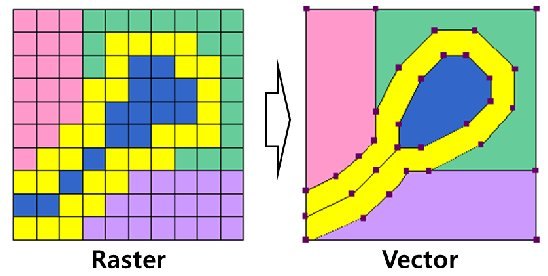
\includegraphics[scale=1.2]{images/medicine/img8.jpg}
    \caption{So sánh ảnh raster và ảnh vector \cite{WinNT2}.}
\end{figure}

\noindent Một ví dụ về đọc và hiển thị ảnh raster bằng python sử dụng opencv.
\vspace{-0.4cm}
\begin{minted}[frame=single,framesep=3pt]{python}
import cv2
import matplotlib.pyplot as plt
img = cv2.imread('img1.png')
\end{minted} 
\vspace{-0.4cm}
Biến img lưu trữ hình ảnh img1.png là một mảng nhiều chiều, muốn hiển thị số chiều của biến img ta chạy lệnh sau:
\vspace{-0.4cm}
\begin{minted}[frame=single,framesep=3pt]{python}
img.shape
=> Output: (384, 430, 3)
\end{minted} 
\vspace{-0.4cm}
Số 384 là chiều rộng của ảnh, số 430 là chiều dài của ảnh, số 3 số là kênh màu  của ảnh.
Để hiển thị hình ảnh dưới dạng mảng nhiều chiều, ta chạy dòng lệnh sau
\vspace{-0.4cm}
\begin{minted}[frame=single,framesep=3pt]{python}
img
array([[[255, 255, 255],
        [255, 255, 255],
        ...,
        [255, 255, 255],
        [255, 255, 255]],
        ...,
        [255, 255, 255],
        [255, 255, 255]]], dtype=uint8)
\end{minted} 
\vspace{-0.4cm}
Để hiển thị hình ảnh, ta chạy những dòng lệnh sau:
\vspace{-0.3cm}
\begin{minted}[frame=single,framesep=3pt]{python}
plt.imshow(cv2.cvtColor(img, cv2.COLOR_BGR2RGB))
plt.show()
\end{minted} 
\vspace{-0.4cm}

\begin{figure}[H]
    \centering
    
\includegraphics[width=8cm]{images/medicine/img10.jpg}
    \caption{Một hình ảnh raster (Nguồn: internet)}
\end{figure}

\subsection{Định nghĩa và phân loại ảnh y khoa}
Ảnh y khoa là kỹ thuật và quy trình tạo hình ảnh trực quan về bên trong của cơ thể để phân tích lâm sàng và can thiệp y tế, cũng như biểu thị trực quan chức năng của một số cơ quan hoặc mô sinh lý học. Hình ảnh y khoa nhằm tìm kiếm các cấu trúc bên trong được che giấu bởi da và xương cũng như chẩn đoán và điều trị bệnh. Hình ảnh y khoa cũng thiết lập một cơ sở dữ liệu giải phẫu học và sinh lý học bình thường để phục vụ việc xác định các bất thường trong mô sinh học. Mặc dù hình ảnh của các cơ quan và mô bị loại bỏ có thể được thực hiện vì lý do y tế, các thủ tục như vậy thường được coi là một phần của bệnh lý thay vì hình ảnh y khoa.

\subsubsection{Các loại ảnh y khoa phổ biến bao gồm}
\paragraph{Ảnh chụp cắt lớp vi tính (CT)}Sử dụng tia X để tạo ra hình ảnh cắt ngang của cơ thể. Nguồn tia X và máy dò quay xung quanh bệnh nhân tạo ra chùm tia X hình quạt hẹp đi qua một phần của cơ thể bệnh nhân để tạo ra một bức ảnh chụp nhanh. Những ảnh chụp nhanh này sau đó được đối chiếu thành một hoặc nhiều hình ảnh của các cơ quan nội tạng.\par

Quét CT cung cấp độ rõ nét cao hơn so với tia X thông thường với hình ảnh chi tiết hơn về các cơ quan nội tạng, xương, mô mềm và mạch máu trong cơ thể. Lợi ích của việc sử dụng CT scan vượt xa các rủi ro như với tia X, bao gồm nguy cơ gây ung thư, gây hại cho trẻ chưa sinh hoặc phản ứng với chất tương phản hoặc thuốc nhuộm có thể được sử dụng. Trong nhiều trường hợp, việc sử dụng CT scan ngăn ngừa sự cần thiết phải phẫu thuật thăm dò
\vspace{-0.7cm}
\paragraph{Ảnh MRI (Magnetic Resonance Imaging)}Sử dụng từ trường và sóng vô tuyến mạnh để tạo ra hình ảnh của cơ thể không thể nhìn rõ bằng tia X hoặc CT, tức là nó cho phép nhìn thấy bên trong khớp hoặc dây chằng hơn chỉ là bên ngoài. Thường được sử dụng để kiểm tra cấu trúc cơ thể bên trong để chẩn đoán đột quỵ, khối u, chấn thương tủy sống, phình động mạch và chức năng não.
\vspace{-0.7cm}                
\paragraph{Siêu âm (Ultrasound)}là hình thức lấy ảnh y tế an toàn nhất. Siêu âm sử dụng sóng âm chứ không phải bức xạ ion hóa. Các sóng âm thanh tần số cao được truyền từ đầu dò đến cơ thể thông qua gel dẫn, các sóng đó sẽ bật trở lại khi chúng chạm vào các cấu trúc khác nhau trong cơ thể và được sử dụng để tạo ra hình ảnh để chẩn đoán.
\vspace{-0.7cm}                
\paragraph{Ảnh X-ray} Là phương pháp lâu đời nhất nhưng đến nay vẫn được sử dụng nhiều nhất. Tia X hoạt động trên một bước sóng và tần số mà chúng ta không thể nhìn thấy bằng mắt thường, nhưng có thể xuyên qua da để tạo ra một bức tranh về những gì diễn ra bên dưới. Thường được sử dụng để chẩn đoán các vấn đề với hệ thống xương, tia X cũng có thể được sử dụng để phát hiện ung thư thông qua chụp nhũ ảnh và các vấn đề tiêu hóa thông qua nuốt barium và thụt.\par

X-quang được sử dụng rộng rãi vì chi phí thấp, nhanh chóng và tương đối dễ dàng cho bệnh nhân chịu đựng. Tuy nhiên, có những rủi ro liên quan đến việc sử dụng bức xạ để chụp ảnh tia X. Mỗi khi bệnh nhân chụp X-quang họ sẽ nhận được một liều phóng xạ. Điều này có thể tiếp tục gây ra ung thư hoặc đục thủy tinh thể do phóng xạ sau này trong cuộc sống hoặc gây ra sự xáo trộn trong sự phát triển của phôi thai hoặc thai nhi ở một bệnh nhân mang thai. Hầu hết các rủi ro này được giảm thiểu bằng cách chỉ sử dụng tia X khi thực sự cần thiết và che chắn chính xác cho cơ thể.

\subsection{Ảnh chụp cắt lớp vi tính}
%\Tham khảo tại :  sách Computed Tomography for Technologists
Định nghĩa CT (Computed Tomography): Sử dụng máy vi tính để xử lý thông tin thu được sau khi chiếu chùm tia X qua khu vực giải phẫu. \par
So sánh CT và X-quang thông thường: X-quang thông thường mô tả một vật 3 chiều như một hình ảnh 2 chiều. Điều này dẫn đến việc các mô bị đặt chồng chất lên nhau, đây là một hạn chế lớn của ảnh X-quang thông thường. Do đó, ảnh chụp cắt lớp vi tính sẽ khắc phục vấn đề này bằng cách quét các phần mỏng của cơ thể bằng chùm tia X hẹp xoay quanh cơ thể, tạo ra hình ảnh của từng mặt cắt. Một ưu điểm khá là kỹ thuật chụp CT có khả năng phân biệt được giữa hai mô có mật độ tương đồng, loại bỏ được các cấu trúc chồng chất. \par

\begin{figure}[H]
    \centering
    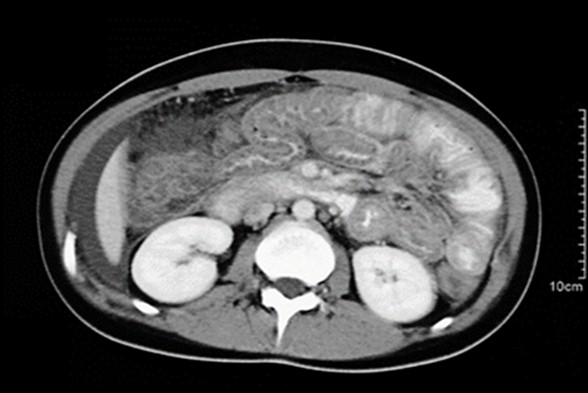
\includegraphics[width=10cm]{images/medicine/img9.jpg}
    \caption{Hình ảnh CT khoan bụng của một người trưởng thành \cite{ctimage}. }
\end{figure}

\subsubsection{Chất lượng ảnh CT thường được đánh giá bằng những tiêu chí sau:}
\paragraph{Độ phân giải không gian}là một thuật ngữ khác được sử dụng để phân giải chi tiết. Độ phân giải không gian là khả năng của hệ thống phân biệt được những hình dạng riêng biệt, những vật thể nhỏ nằm gần nhau. Độ phân giải không gian có thể được đo bằng hai phương pháp. Nó có thể được đo trực tiếp, hoặc có thể được tính từ phân tích sự lan truyền thông tin trong hệ thống.  Điều này phân tích dữ liệu sau được gọi là hàm truyền điều chế (MTF). Bằng cách định lượng độ phân giải không gian ở một trong những cách, có thể so sánh hiệu năng của hệ thống với hệ thống CT khác hoặc cùng hệ thống vào một ngày khác.
\vspace{-0.7cm}
\paragraph{Độ phân giải tương phản}là khả năng của hệ thống có thể phân biệt những vật thể có cùng mật độ trên hình ảnh. 

\subsection{Đơn vị Hounsfield}
Hounsfield unit đo mức độ hấp thụ tia X của một đối tượng. Trong X-quang thông thường, ta phải xác định trực quan những sắc thái của màu xám và phỏng đoán mật độ của những cấu trúc bên trong cơ thể bệnh nhân. Trong CT, chúng ta có thể định lượng khả năng làm suy giảm một chùm tia X của một đối tượng nhất định. Các phép đo được thể hiện bằng đơn vị Hounsfield (HU), được đặt theo tên của Godfrey Hounsfield, một trong những người tiên phong trong việc phát triển CT. Các đơn vị này cũng được gọi là số CT hoặc giá trị mật độ. Có thể hiểu HU là định lượng mức độ mà một cấu trúc làm suy giảm chùm tia X.\par

Hounsfield đã được gán nước cất với số 0, số 1000 cho xương và số $-1000$ cho không khí. Các vật thể có mức độ suy giảm chùm tia nhỏ hơn nước sẽ có giá trị Hounsfield âm, ngược lại sẽ có giá trị dương. Giá trị đơn vị của Hounsfield liên quan trực tiếp đến hệ số suy giảm tuyến tính: 1 HU bằng chênh lệch 0,1 phần trăm  giữa hệ số suy giảm tuyến tính của mô so với hệ số suy giảm tuyến tính của nước. Hệ số hấp thụ tuyến tính là lượng chùm tia x bị tán xạ hoặc bị hấp thụ trên một đơn vị độ dày của chất hấp thụ. 

\begin{figure}[H]
    \centering
    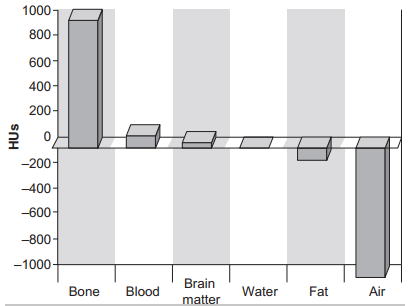
\includegraphics[width=12cm]{images/medicine/img2.png}
    \caption{Các đơn vị Hounsfield gần đúng \cite{ctimage}. }
\end{figure}
\vspace{-0.5cm}
Các ảnh CT tuân theo chuẩn DICOM (Digital Image and Communications in Medicine) thông thường sẽ có một kênh và được biểu thị bằng số nguyên 16-bit và được tổ chức xếp nhiều ảnh với nhau thành ảnh 3 chiều. Lúc này điểm ảnh pixel trên không gian hai chiều sẽ trở thành điểm ảnh voxel trên không gian ba chiều. Ảnh CT 3 chiều này sẽ đi kèm theo các thông tin về khoảng cách thực tế giữa hai voxel gần nhau trong không gian ba chiều. Nhờ đó ta có thể tính được diện tích và thể tích của vật thể nhờ vào số voxel của ảnh đó.\par

Mỗi lát cắt CT đại diện cho một vùng cụ thể trong cơ thể bệnh nhân. Độ dày của vùng này tương ứng với chiều dài theo trục Z. Dữ liệu thu thập từ máy CT được phân thành những phần tử: chiều dài đại diện bởi trục X, chiều cao đại diện bởi trục Y. Mỗi một hình vuông 2 chiều này là 1 pixel. Tập hợp hàng nghìn pixel tạo ra hình ảnh CT được hiển thị trên màn hình máy CT. Nếu mỗi pixel được bao gồm cả trục Z, thì lúc này pixe được gọi là voxel.
\begin{figure}[H]
    \centering
    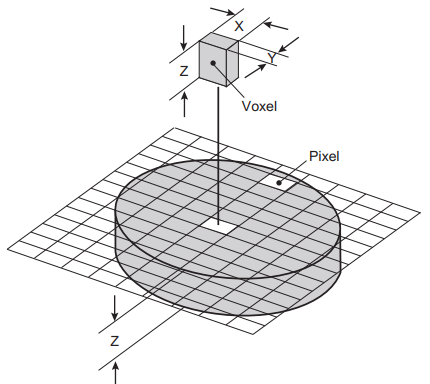
\includegraphics[width=8cm]{images/medicine/img1.png}
    \caption{Dữ liệu hình thành lát cắt CT được chia thành các phần tử \cite{ctimage}.} 
\end{figure}

% \subsection{Các loại dữ liệu}
% \subsubsection{Dữ liệu thô}
% Hàng ngàn bit dữ liệu thu thập được từ hệ thống gọi là dữ liệu thô. Quá trình sử dụng dữ liệu thô để tái tạo hình ảnh gọi là quá trình dựng ảnh. Việc xây dựng ảnh được tự động tạo ra trong quá trình quét thường được gọi là tái thiết trong tương lai (prospective reconstruction). Dữ liệu thô tương tự có thể được sử dụng sau này để tạo ra một hình ảnh mới. Quá trình này được gọi là tái thiết hồi cứu (retrospective reconstruction). Bởi vì dữ liệu thô bao gồm tất cả các phép đo thu được từ máy quét, nhiều hình ảnh có thể được tạo từ cùng một dữ liệu.
% \vspace{-0.5cm}
% \subsubsection{Dữ liệu hình ảnh}
% Để tạo thành một hình ảnh, máy tính gán một giá trị (đơn vị Hounsfield) cho mỗi pixel). Giá trị này (số mật độ), là trung bình của tất cả các phép đo suy giảm cho pixel đó. Pixel hai chiều đại diện cho một phần ba chiều của mô bệnh nhân. Giá trị pixel đại diện cho tỷ lệ  lượng năng lượng tia X đi qua mô và đến máy thu. Khi dữ liệu được tính trung bình để mỗi pixel có một số cụ thể, một hình ảnh có thể được hình thành. Dữ liệu trong hình ảnh này gọi là dữ liệu hình ảnh. Dữ liệu hình ảnh đòi hỏi khoảng 1/5 dung lượng bộ nhớ so với dữ liệu thô. Dữ liệu hình ảnh cho phép các phép đo như đơn vị Hounsfield, độ lệch chuẩn, khoảng cách nhưng không thể phân tích những thứ không quan sát được trên hình ảnh. Tóm lại, một giá trị đơn vị Hounsfield sẽ được gán cho một pixel. 

\section{Kỹ thuật phân đoạn ảnh}
\subsection{Định nghĩa}
Trong lĩnh vực xử lý ảnh, kỹ thuật phân đoạn ảnh (image segmentation) hay còn gọi pixed-level classification thực hiện nhiệm vụ phân vùng các đối tượng trong ảnh thành tập hợp các pixel. Điều đó có nghĩa là chúng ta cần phân biệt được các đối tượng quan tâm (gan, mạch máu,...) và phần còn lại của ảnh (nền ảnh). \par

Một cách hiểu khác, nhiệm vụ của nó là ta xác định trong có cái gì trong hình này, và nó nằm ở đâu trong ảnh. \par

Cụ thể hơn, mục đích của phân đoạn ảnh là gắn nhãn cho từng pixel (voxel cho ảnh 3D). Bởi vì việc dự đoán lớp của từng pixel trong ảnh nên nó còn có một tên khác dense prediction.

\begin{itemize}
    \item[] Kỹ thuật phân đoạn ảnh mang lại nhiều hiệu quả trong nhiều lĩnh vực:
	\item Phát triển xe tự hành (autonomous vehicles) như việc nhận diện các biển báo, người qua đường, phát hiện đèn dừng xe,... 
	\item Hình ảnh y tế: phát hiện khối u trong não, gan,... xây dựng lại hệ thống mạch máu, hiển thị một cách trực quan các bộ phận bên trong cơ thể. Từ đó hỗ trợ các bác sĩ đưa ra chuẩn đoán chính xác hơn, chuẩn bị chiến lược cần thiết trước quá trình phẫu thuật.
	\item Một số ứng dụng nhận dạng khác như: nhận dạng vân tay, khuôn mặt, võng mạc,...
\end{itemize}

\subsection{Hướng tiếp cận phân đoạn ảnh}
\subsubsection{Phân đoạn dựa theo ngưỡng}
Là thuật toán phân đoạn đơn giản nhất. Phương pháp phân đoạn theo ngưỡng dựa trên những giá trị cường độ của các điểm ảnh và những điểm lân cận với nó liệu có lớn hơn hay nhỏ hơn một ngưỡng đang xét để phân loại pixel đó thuộc lớp nào.

\newpage
% Để việc phân đoạn theo ngưỡng đạt kết quả cao, việc chọn ngưỡng cho phù hợp là bài toán máy tính cần xử lý một cách tự động. Do đó có sự xuất hiện của nhiều thuật toán có thể kể đến như: 
% \begin{itemize}
% 	\item Phương pháp dựa trên cụm (Clustering-based methods).
% 	\item Phương pháp dựa trên lược đồ Histogram (Histogram shape-based methods).
% 	\item Phương pháp dựa trên thuộc tính đối tượng (Object Attribute-based methods).
% 	\item Phương pháp dựa trên Entropy (Entropy-based methods).
% 	\item Phương pháp không gian (Spatial methods).
% 	\item Phương pháp dựa trên tính chất cục bộ (Local method).
% \end{itemize}

\subsubsection{Phân đoạn dựa theo miền đồng nhất}
Là kỹ thuật phân đoạn ảnh dựa trên yếu tố về không gian, màu sắc để ước lượng tính đồng nhất của miền. Việc lựa chọn các tính chất để phân vùng sẽ xác định tiêu chuẩn của vùng đó.
Các phương pháp có thể kể đến như:
\begin{itemize}
	\item Phương pháp tách cây tứ phân.
	\item Phương pháp phân vùng hợp.
	\item Phương pháp tách hợp (split-merge).
\end{itemize}

\subsubsection{Phân đoạn dựa trên mô hình mạng học sâu (Deep Learning)}
Các kỹ thuật phân đoạn truyền thống kể trên phần nào giải quyết được bài toán nhưng độ chính xác chưa cao, dễ bị sai khi bức ảnh không có sự rõ ràng màu sắc, độ tương quan... giữa các đối tượng.\par 

Hiện nay, với sự phát triển của mô hình mạng học sâu và sự tiến bộ về phần cứng đã đưa các giải pháp học máy hứa hẹn hơn, độ chính xác của mô hình đã tăng một cách đáng kể so với các phương pháp truyền thống. Trong các cuộc thi xử lý ảnh gần đây, các phương pháp dựa trên mạng học sâu luôn giành kết quả đứng đầu ở hầu hết các bài toán không chỉ xử lý ảnh mà còn cả xử lý ngôn ngữ tự nhiên, xử lý tín hiệu. Chi tiết ta có thể tham khảo thêm tại bài báo đánh giá các phương pháp mô hình học sâu trên ảnh y khoa tại đây \cite{reviewDLmedical}.

\section{Mạng học sâu}
Học sâu (Deep learning) là một kĩ thuật của máy học (Machine learning) dựa trên một tập hợp các thuật toán với mục tiêu mô hình dữ liệu trừu tượng thông qua nhiều lớp xử lý phức tạp (nhiều lớp biến đổi phi tuyến).\par

Một trong những phương pháp học sâu thành công nhất là mạng nơ-ron nhân tạo (Artificial Neural Network) hay cao hơn là Deep Neural Network được đề xuất bởi 2 người đoạt giải Nobel David H. Hubel và Torsten Wiesel. \par

Mạng nơron nhân tạo là một mô hình toán học (hay mô hình tính toán) được xây dựng dựa trên ý tưởng của mạng nơ-ron sinh học, bao gồm có một nhóm các nơ-ron nhân tạo (unit) nối với nhau và xử lý thông tin bằng cách truyền theo các kết nối và tính giá trị mới tại các nút. Trong nhiều trường hợp, mạng nơ-ron nhân tạo là một hệ thống thích ứng (adaptive system) tự thay đổi cấu trúc của mình dựa trên các thông tin bên ngoài hay bên trong chảy qua mạng trong quá trình học. \par

Mạng nơ-ron giống như bộ não con người, được học bởi kinh nghiệm (thông qua huấn luyện), có khả năng lưu giữ những kinh nghiệm tri thức và sử dụng những tri thức đó trong việc dự đoán các dữ liệu chưa biết (unseen data). Kiến trúc chung của một mạng nơron nhân tạo gồm 3 thành phần đó là: lớp đầu vào (input layer), lớp ẩn (hidden layer) và lớp đầu ra (output layer). 

\subsection{Thách thức đối với mạng học sâu}
Một mô hình học sâu đủ lớn có thể mô hình hóa bất kì mối quan hệ nào của dữ liệu. Tuy nhiên để huấn luyện được nó là một thách thức lớn, nhiều vấn đề có thể nảy sinh trong quá trình huấn luyện như tình trạng quá khớp (overfitting) hay thời gian tính toán quá dài, có khả năng không hội tụ tại nghiệm tối ưu. \par

Các mô hình có thiên hướng xảy ra hiện tượng quá khớp vì được thêm các lớp trừu tượng, mà cho phép chúng thực hiện mô hình hóa phụ thuộc vào các ngoại lệ của dữ liệu huấn luyện. Để tránh overfitting, có rất nhiều kỹ thuật được sử dụng, điển hình là cross-validation và regularization. Ngoài ra còn một phương pháp khác gần đây được áp dụng rất phổ biến dropout regularization. Dropout là một phương pháp tắt ngẫu nhiên các unit trong mô hình mạng. Điều này không những giúp phá vỡ các phụ thuộc từ các ngoại lệ của dữ liệu có thể xảy ra mà còn giúp lượng tính toán giảm đi đáng kể.

\subsection{Ứng dụng mạng học sâu trong phân đoạn ảnh}
Một hướng tiếp cận phổ biến trong bài toán phân đoạn ảnh dựa trên mạng học sâu là xây dựng mô hình theo kiến trúc Encoder-Decoder. Có nghĩa là, kiến trúc tổng thể của ta gồm 2 phần chủ yếu, một phần đại diện cho việc mã hóa đặc trưng dữ liệu có ích (có ý nghĩa cho việc phân loại từng pixel), phần còn lại tái cấu trúc (khôi phục) bản đồ đặc trưng tương ứng với ảnh đầu vào ban đầu. \par

Một số kiến trúc mạng được sử dụng cho bài toán phân đoạn ảnh phổ biến như sau, chi tiết có thể kham khảo thêm tại bài báo gốc: 
\vspace{-0.5cm}
\begin{itemize}
    \item U-Net: Convolutional Networks for Biomedical Image Segmentation \cite{Unet}.
	\item Fully Convolutional Networks for Semantic Segmentation (FCN) \cite{FCN}.
	\item Mask R-CNN \cite{RCNN}.
\end{itemize}

\subsubsection{Một số lớp chính trong mạng học sâu}
\paragraph{Lớp tích chập}là lớp tính toán dùng để trích xuất các đăc trưng từ ảnh, từ đó có thể đưa ra giá trị dự báo phân lớp dựa trên các đặc trưng đã trích xuất được. Trong lớp tính toán tích chập chứa các tham số (kernel) đã được học để tự điều chỉnh lấy ra những thông tin chính xác nhất mà không cần chọn các đặc trưng cụ thể (feature).\par

Phép tích chập được thực hiện trên giá trị đầu vào của dữ liệu và kernel (filter) để tạo ra một bản đồ đặc trưng (feature map). Một mạng tích chập cần nhiều feature map, thực hiện tương tự quá trình tích chập cho từng đặc trưng khác nhau, kết quả thu được là một tập hợp các đặc trưng có ích, tương ứng với mỗi bộ lọc.\par

Về mặt toán học, tích chập của hàm số $f$ và $g$ được viết là $ (f\ast g)$ có thể thể hiện như sau:
\begin{equation}
	{(f*g)(t)\ \ } {\stackrel {\mathrm {def} }{=}} {\ \ \int_{-\infty }^{\infty }f(\tau )\,g(t-\tau ) d\tau}
\end{equation}

Trong đó f đại diện cho ảnh ban đầu, g là bộ lọc của phép tích chập (filter).

Bộ lọc (filters) có kích thước nhỏ hơn so với ảnh (thường ma trận 3x3 hoặc 5x5). Tiến hành tích chập, bộ lọc sẽ dịch chuyển trên ảnh theo bước trượt chạy dọc theo ảnh và quét toàn bộ ảnh thu được feature map. Để tính toán sự khớp của một đặc trưng đối với một hình ảnh, ta thực hiện nhân mỗi điểm ảnh trong feature với giá trị của điểm ảnh tương ứng trong hình ảnh và lấy tổng của chúng.

\begin{figure}[H]
	\begin{center}
		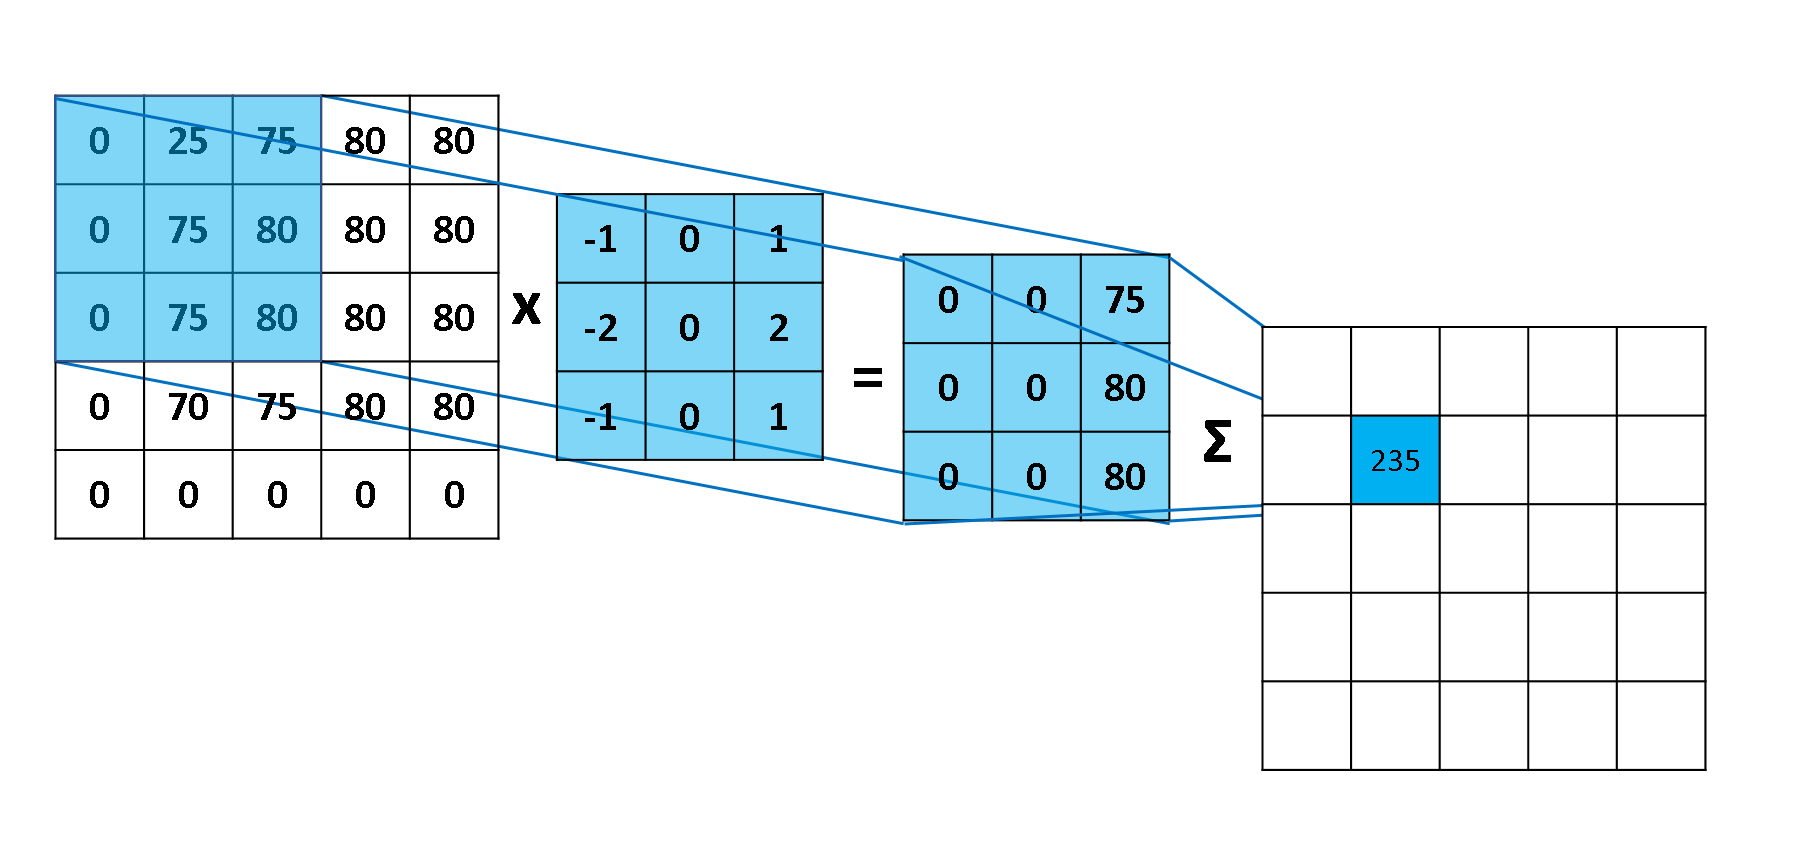
\includegraphics[width=12cm]{images/blood/convExample.png}
		\caption{Ví dụ minh họa về phép tích chập \cite{CNN}}
	\end{center}
\end{figure}

Thực hiện tương tự quá trình tích chập cho từng đặc trưng khác, kết quả thu được là một tập hợp các đặc trưng được trích xuất tương ứng với mỗi bộ lọc. 

Có hai dạng tính tích chập chính mà ta thường dùng là Valid và Same. Hai dạng cho ảnh kết quả có kích thước khác nhau:
\begin{itemize}
	\item Dạng Valid: kernel được trượt trên toàn ảnh, sau khi tính tích chập kết quả sẽ nhỏ hơn kích thước ảnh ban đầu. Với ảnh đầu vào có kích thước (m x m), kernel kích thước (n x n) thì ảnh đầu ra sẽ có kích thước (m-n+1)x(m-n+1). 
	\item Dạng Same: trước khi tính tích chập, ảnh sẽ được đệm (padding) thêm các giá trị (thường các giá trị này sẽ là 0 hoặc 1) để tăng kích thước ảnh, sao cho sau khi thực hiện Convolution, kích thước ảnh kết quả sẽ bằng với kích thước ảnh ban đầu.
\end{itemize}

\paragraph{Lớp gộp (Pooling layer)}có tác dụng giúp loại bỏ những thông tin không cần thiết, thường được sử dụng sau lớp tích chập. Rất hữu ích khi làm giảm độ phức tạp khi tính toán, tuy nhiên nếu lạm dụng nhiều có thể làm mất dữ liệu. \par

Trong lớp này sử dụng cửa sổ trượt, mỗi lần trượt theo một bước trượt (stride) cho trước. Khác với lớp tích chập, lớp gộp không tính tích chập mà tiến hành lấy mẫu (sub-sampling). Một giá trị đại diện thông tin ảnh tại vùng ảnh đó được giữ lại. Một số phương pháp phổ biến được sử dụng trong lớp gộp là max pooling (lấy giá trị lớn nhất), min pooling (lấy giá trị nhỏ nhất) và average pooling (lấy giá trị trung bình). \par

Ví dụ minh họa: mô hình có kích thước (4x4), lớp gộp dùng bộ lọc (2x2), bước trượt là 2, sử dụng phương pháp Max Pooling. Tiến hành gộp ảnh, giá trị lớn nhất trong vùng cửa sổ (2x2) giới hạn bởi bộ lọc được giữ lại, làm đầu ra. Sau lớp gộp, kích thước ảnh giảm đi 2 lần mỗi chiều (2x2). 

\begin{figure}[H]
	\begin{center}
		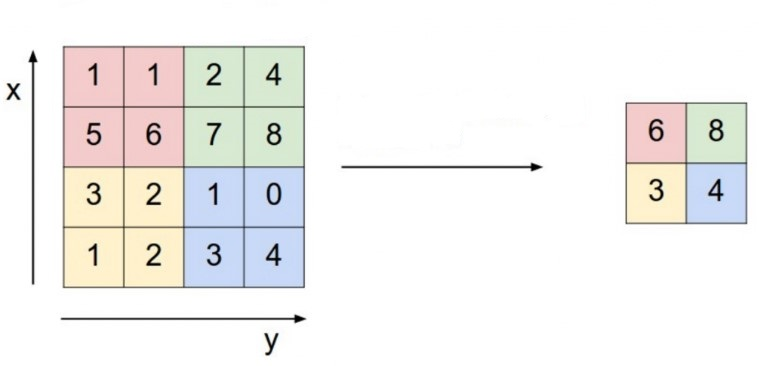
\includegraphics[width=12cm]{images/blood/maxpool.jpg}
		\caption{Minh họa lớp Max Pooling \cite{CNN}}
	\end{center}
\end{figure}

Khi dữ liệu ảnh có kích thước lớn, thực hiện qua nhiều lớp gộp sẽ thu nhỏ, giảm kích thước dữ liệu. Từ đó làm giảm lượng tham số, tăng hiệu quả tính toán và góp phần kiểm soát hiện tượng quá khớp (overfitting). \par

Ta có thể thấy, sau khi chạy qua các lớp gộp các đặc trưng khác nhau sẽ nằm gần lại với nhau hơn. Nhờ đó, lớp tích chập phía sau sẽ trích xuất được thông tin ở vùng lớn hơn vùng ở lớp đầu. Vì vậy, qua nhiều lớp gộp và tích chập, đặc trưng thu được sẽ có ý nghĩa toàn cục hơn là ý nghĩa chi tiết. \par

Lớp gộp sẽ cho bạn tính bất biến đối với phép dịch chuyển (translation), phép quay (rotation) và phép co giãn (scaling). Tính kết hợp cục bộ cho ta các cấp độ biểu diễn thông tin từ mức độ thấp đến mức độ cao và trừu tượng hơn thông qua lớp tích chập từ các bộ lọc.

%%%%%%%%%%%%%%% (start) metric to evaluate 
\newpage
\section{Các phương pháp đánh giá mô hình phân đoạn ảnh}\label{evaluation-methods}
Khi xây dựng một mô hình mạng học sâu, chúng ta cần một công cụ để có thể đánh giá xem mô hình có hoạt động hiệu quả hay không đồng thời giúp chúng ta đánh giá khả năng giữa các mô hình. \par

Hiệu năng của một mô hình được đánh giá trên tập dữ liệu kiểm thử (test dataset). Giả sử khi cho đầu vào chạy qua mô hình ta sẽ được đầu ra của tập kiểm thử là các dự đoán của mô hình (gọi là y predict). Đó là một bức ảnh dưới dạng tensor với những giá trị xác xuất dự đoán thuộc lớp nào. Còn y true đại diện cho tensor với nhãn thật của dữ liệu. Do đó ta cần so sánh giữa 2 tensor y predict và y true.\par

\subsection{Ma trận nhầm lẫn}
Khi đánh giá một mô hình mạng học sâu, chúng ta thường đề cập đến một thuật ngữ gọi là ma trận nhầm lẫn (\textbf{confusion matrix}) \cite{confution}. Một bảng dùng để mô tả hiệu suất của một mô hình phân loại trên tập dữ liệu đã biết kết quả đúng, giúp ta có cái nhìn trực quan về hiệu suất các giải thuật.
\begin{table}[H]
\centering
\begin{tabular}{l|l|c|c|}
	\multicolumn{2}{c}{}	&	\multicolumn{2}{c}{Giá trị thực}	\\
	\cline{3-4}
	\multicolumn{2}{c|}{}					   & Positive &	Negative \\
	\cline{2-4}
	\multirow{2}{*}{Giá trị dự đoán}& Positive & TP 	  & FP 		 \\
	\cline{2-4}
									& Negative & FN		  & TN	 	 \\
	\cline{2-4}
\end{tabular}
\caption{Ma trận nhầm lẫn}
\label{confution_matrix}
\end{table}
\vspace{-5mm}
Cụ thể hơn, khi xét một bài toán phân loại 2 lớp: trong đó một lớp nghiêm trọng hơn lớp kia cần được đự doán chính xác. Giả sử ta đang xét bài toán phân loại gồm 2 lớp: ung thư (positive), không ung thư (negative).
\begin{itemize}[noitemsep, topsep=0pt]
	\item Positive: Đối tượng được gán nhãn là ung thư.
	\item Negative: Đối tượng được gán nhãn là không phải ung thư.
	\item True Positive (TP): Khi mô hình dự đoán đúng đối tượng đó là ung thư.
	\item False Positive (FP): Khi mô hình dự đoán đối tượng đó là ung thư nhưng thực sự nó là không phải là ung thư.
	\item True Negative (TN): Khi mô hình dự đoán đúng đối tượng đó là không phải ung thư.
	\item False Negative (FN): Khi mô hình dự đoán đối tượng đó là không phải ung thư nhưng thực sự nó là ung thư.
\end{itemize}

Bên cạnh đó, các chỉ số False Positive Rate (tỉ lệ báo động nhầm), False Negative Rate (tỉ lệ bỏ sót) cũng đáng được quan tâm. 
\begin{equation}
	\mathrm{FPR} = \mathrm{\frac{FP}{FP + TN}} \hspace{0.5cm}
	\mathrm{FNR} = \mathrm{\frac{FN}{TP + FN}}
\end{equation} 

Ví dụ, trong bài toán xác định có bệnh ung thư hay không thì việc không bị sót quan trọng hơn là việc chẩn đoán nhầm âm tính thành dương tính. Hay trong bài toán lọc email rác thì việc cho nhầm email quan trọng vào thùng rác nghiêm trọng hơn việc xác định một email rác là email thường. \par

Với các bài toán có nhiều lớp dữ liệu, ta có thể xây dựng bảng True/False Positive/Negative cho mỗi lớp nếu coi lớp đó là lớp Positive, các lớp còn lại gộp chung thành lớp Negative.

% \subsection{Pixel Accuracy}
% Một cách đánh giá cơ bản cho bài toán phân đoạn ảnh là tính tỉ lệ pixels (voxel) của ảnh đó được phân loại đúng.
% Tuy nhiên trong bài toán phân đoạn (còn gọi dense prediction) đôi khi độ đo accuracy không thể hiện được mô hình liệu có hiệu suất tốt hay không vì xuất hiện các vấn đề như: mất cân bằng dữ liệu (một lớp trong ảnh có tỉ lệ xuất hiện quá nhỏ so với lớp còn lại). Miền giá trị của độ đo [0,1] (hay $0-100\%$).
% \begin{equation}
% \begin{aligned}
% 	\mathrm{accuracy} = \mathrm{\frac{TP + TN}{TP + TN + FP + FN}}
% \end{aligned}
% \end{equation}

\subsection{Độ chính xác và độ truy hồi }
Độ chính xác (precision) được định nghĩa là tỉ lệ số điểm được đánh giá là True Positive trong những điểm được phân loại là positive.
Độ truy hồi (recall) được định nghĩa là tỉ lệ số điểm được đánh giá là true positive trong số những điểm thực sự là positive. 

\begin{equation}
    \mathrm{Precision = \frac{TP}{TP + FP}} \hspace{0.5cm}
    \mathrm{Recall = \frac{TP}{TP + FN}}
\end{equation}

Xét trường hợp precision = 1, có nghĩa là mọi điểm tìm được đều thực sự là positive, tức không có điểm negative nào lẫn vào kết quả. Tuy nhiên vẫn chưa đủ khẳng định là mô hình thực sự tốt, vì nó không đánh giá những điểm positive thật sự đã được phân loại đủ hay chưa. Do đó,nếu một mô hình chỉ tìm được đúng một điểm positive mà nó chắc chắn nhất thì ta không thể gọi nó là một mô hình tốt.
\newpage
Xét trường hợp recall = 1, có nghĩa là mọi điểm positive đều được tìm thấy. Tuy nhiên, đại lượng này lại không đo liệu có bao nhiêu điểm negative bị lẫn trong đó. Nếu mô hình phân loại mọi điểm là positive thì chắc chắn recall = 1, tuy nhiên dễ nhận ra đây là một mô hình cho kết quả cực kì tệ.\par

Một mô hình phân loại tốt là mô hình có cả Precision và Recall đều cao, tức càng gần một càng tốt. Có hai cách đo chất lượng của bộ phân lớp dựa vào Precision và Reall: Precision-Recall curve và F1-score (Dice).
\vspace{-0.25cm}
% \subsection{Intersection over Union (IoU)}
% Độ đo IoU (hay được biết đến Jascard Index \cite{iou}) là một trong những độ đo được sử dụng phổ biến trong bài toán phân đoạn ảnh.\par 

% Ý tưởng cơ bản là IoU là tập hợp những pixel thuộc chung một lớp (phần trùng lắp) giữa giá trị phân đoạn do mô hình dự đoán và nhãn thực (ground truth) của nó. Độ đo này có phần gần giống với hệ số Dice, chúng thường được sử dụng trong hàm đánh giá mất mát trong quá trình huấn luyện. \par

% \begin{equation} 
% \begin{aligned}
% 	\mathrm{IoU} = \frac{|\mathrm{Predict} \cap \mathrm{Target}|}{|\mathrm{Predict} \cup \mathrm{Target}|}
% 				= \mathrm{\frac{TP}{TP + FP + FN}}
% \end{aligned}
% \end{equation}

% Đơn giản hơn, IoU tính số lượng pixel được dự đoán chung lớp của cả giá trị mục tiêu và dự đoán, giá trị này chia cho tổng số pixel được dự đoán là thuộc lớp đó của cả 2 giá trị mục tiêu và dự đoán.

\subsection{Hệ số tương đồng Dice}
Hệ số tương đồng Dice (hay còn gọi F1 Score) là một phương pháp thống kê dùng để đo độ giống nhau giữa hai mẫu được giới thiệu bởi Thorvald Sørensen\cite{dice1} và Lee Raymond Dice\cite{dice}. \par

Hệ số Dice ban đầu được phát triển cho dữ liệu 2 lớp. Có thể tính bằng cách lấy 2 lần khu vực trùng lắp lên nhau của giá trị dự đoán và nhãn thực chia cho tổng số pixel của ảnh. Độ đo có miền giá trị từ [0,1] với giá trị 1 thể hiện cho việc trùng lắp hoàn hảo giữa giá trị dự đoán và giá trị thực.
\begin{equation}
	\mathrm{Dice(A, B)} = \mathrm{\frac{2 * |A \cap B|}{|A| + |B|}}
\end{equation} 

Trong đó, A là một ảnh đầu ra của mô hình, chứa các giá trị xác xuất do mô hình dự đoán có thể đúng hoặc sai. B là một ảnh (gọi là ảnh mục tiêu) chứa tập hợp những giá trị cho từng pixel được gán nhãn bởi chuyên gia. A và B có cùng kích thước. $|\mathrm{A}|$ đại diện cho toàn bộ pixel thuộc ảnh A. \par 

Có thể hiểu đơn giản, $|\mathrm{A} \cap \mathrm{B}|$ đại diện cho tập hợp những pixel thuộc cùng một lớp của tập A và B. 

\hspace{-2.0cm}
\begin{tabular}{c c c c c}
	$\left[
	\begin{matrix}
		0.19 & 0.65 & 0.11 & 0.04\\
		0.55 & 0.55 & 0.67 & 0.12\\
		0.01 & 0.16 & 0.05 & 0.11\\
		0.72 & 0.91 & 0.67 & 0.99
	\end{matrix}
	\right]$ & $*$ &
	$\left[
	\begin{matrix}
		0 & 0 & 0 & 0\\
		1 & 1 & 1 & 1\\
		1 & 1 & 1 & 1\\
		0 & 0 & 0 & 0
	\end{matrix}
	\right]$ & $ \underrightarrow{\mathrm{element-wise}}$ &
	$\left[
	\begin{matrix}
		0	 & 0 	& 0 	& 0\\
		0.55 & 0.55 & 0.67 	& 0.12\\
		0.01 & 0.16 & 0.05 	& 0.11\\
		0 	 & 0 	& 0 	& 0
	\end{matrix}
	\right]$ \\ 
	Prediction &  & Target & sum   & \\
	& & & $ \myarrow[2.6cm] $ & $2.22$ 
\end{tabular}

Để định lượng cho giá trị $|\mathrm{A}|$ và $|\mathrm{B}|$, thông thường một số người chọn việc sử dụng tổng bên cạnh đó một số người lại sử dụng tổng bình phương để tính. Vậy nên cách tốt nhất để biết được nên định lượng bằng cách nào là tốt nhất ta nên thử nghiệm cả hai phương pháp tùy vào nhiệm vụ khác nhau sẽ đem lại kết quả tối ưu khác nhau.

\hspace{1.5cm}
\begin{tabular}{c c c}
	$|\mathrm{A}|$ =& 
	$\left[
	\begin{matrix}
		0.19 & 0.65 & 0.11 & 0.04\\
		0.55 & 0.55 & 0.67 & 0.12\\
		0.01 & 0.16 & 0.05 & 0.11\\
		0.72 & 0.91 & 0.67 & 0.99
	\end{matrix}
	\right]^{2 (optional)}$ & $\underrightarrow{\mathrm{sum}}$ 6.5\\ 
	$|\mathrm{B}|$ =&
	$\left[
	\begin{matrix}
	0 & 0 & 0 & 0\\
	1 & 1 & 1 & 1\\
	1 & 1 & 1 & 1\\
	0 & 0 & 0 & 0
	\end{matrix}
	\right]^{2 (optional)}$ & $\underrightarrow{\mathrm{sum}}$ 8
\end{tabular}

Một cách thể hiện khác dựa trên ma trận nhầm lẫn để tính hệ số Dice theo công thức sau:
\begin{equation}
	\mathrm{Dice} = \mathrm{\frac{2TP}{2TP + FP + FN}}
\end{equation}

\subsection{Chỉ số lỗi trùng thể tích}
Chỉ số lỗi trùng thể tích (Volumetric Overlap Error), được tính bằng cách lấy tổng số voxel giao giữa dự đoán và nhãn chia cho tổng số voxel hợp giữa dự đoán và nhãn, lấy 1 trừ kết quả đó ta được giá trị VOE.
\begin{align}
    % VOE = (1 - \frac{|\mathrm{Predict} \cap \mathrm{Target}|}{|\mathrm{Predict} \cup \mathrm{Target}|})*100\%
    \mathrm{VOE} &= 1 - \mathrm{\dfrac{TP}{TP + FN + FP}}
\end{align}

Với TP là số lượng điểm ảnh True Positive, FN là số lượng điểm ảnh False Negative và FP là số lượng điểm ảnh False Positive. Giá trị này là 0 khi phân đoạn hoàn hảo và là 1 (giá trị thấp nhất) khi không có sự chồng chéo nào giữa dự đoán và nhãn.

\subsection{Chỉ số sai khác thể tích}
Chỉ số sai khác thể tích (Volume Difference - VD), đơn vị phần trăm, được tính bằng hiệu số số voxel của dự đoán và nhãn, chia cho số voxel của nhãn..
\begin{align}
    % VD = (\frac{|\mathrm{Predict}| - |\mathrm{Target}|}{|\mathrm{Target}|})*100\%
    \mathrm{VD} &= \mathrm{\dfrac{FP - FN}{TP + FN}}
\end{align}
Với TP là số lượng điểm ảnh True Positive, FN là số lượng điểm ảnh False Negative và FP là số lượng điểm ảnh False Positive. Chỉ số này nhận giá trị âm khi thể tích phân đoạn nhỏ hơn thể tích nhãn và nhận giá trị dương khi thể tích phân đoạn lớn hơn thể tích nhãn.

	\chapter{CÁC NGHIÊN CỨU LIÊN QUAN}\label{chapter:related_works}
\section{Mô hình mạng U-Net}
Mô hình mạng U-Net được giới thiệu trong bài báo ``U-Net: Convolutional Networks for Biomedical Image Segmentation'' vào ngày 18 tháng 5 năm 2015 bởi Olaf và các cộng sự \cite{Unet}. Tên mạng Unet xuất phát từ hình dáng chữ U của kiến trúc mạng, gồm 2 phần chính là mã hóa (Encoder) và giải mã (Decoder). Điểm đặc biệt của mạng U-Net là trong quá trình giải mã, mạng sử dụng lối tắt để kết hợp các đặc trưng được trích xuất từ các tầng tương ứng trong quá trình phần mã hóa. Bên cạnh đó, tác giả còn đề xuất hàm đánh giá mất mát có trọng số dựa trên hàm Binary Cross Entropy với mục tiêu tăng trọng số giữa các điểm biên của các tế bào. Qua đó kết quả phân đoạn tế bào được làm tốt hơn đáng kể.

\subsection{Kiến trúc mạng}
Kiến trúc mạng bao gồm 2 phần chính: phần mã hóa và phần giải mã. Phần mã hóa dựa theo kiến trúc cơ bản của mạng tích chập nơ-ron. Sáu thao tác chính trong mạng Unet bao gồm: Phép tích chập, phép pooling, phép concatetation (kết hợp), phép crop, phép up-conv (deconvolution) và phép ReLU.

\begin{figure}[H]
    \centering
    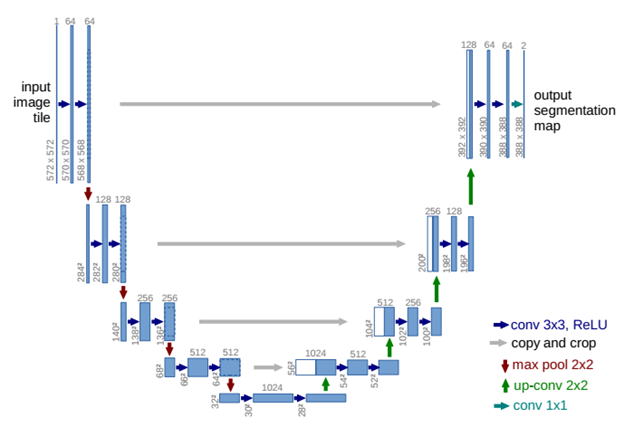
\includegraphics[width=14cm]{images/medicine/img3.png}
    \caption{Kiến trúc mô hình mạng Unet \cite{Unet}.}
\end{figure}

\begin{itemize}
    \item Phần mã hóa (Encoder):\\
    Bao gồm 3 phép ReLU, max pooling, convolution. Ở mỗi phép tích chập, Unet sử dụng kernel size (3x3) và unpadded convolution, tiếp theo sau tích chập là phép ReLU (rectified linear unit) và phép max pooling (2x2) với stride bằng 2 để giảm kích thước mẫu. Sau mỗi bước giảm kích thước mẫu, ta tiến hành nhân đôi số feature channels. 
    
    \item Phần giải mã (Decoder):\\
    Mỗi bước trong phần giải mã bao gồm một phép upsampling  của feature map, tiếp theo là một phép tích chập với kernel size (2x2), sau đó giảm số feature channels xuống một nửa. Mỗi phép concatenation sẽ kết hợp feature map ở phần giải mã với feature map tương ứng ở phần mã hóa (đã được copy và crop). Sau đó thực hiệp phép ReLU. 
\end{itemize}

\newpage

\subsection{Quá trình huấn luyện và hàm lỗi}
Hàm năng lượng $E$ được tính bởi pixel-wise soft-max trên feature map cuối cùng dựa trên hàm đánh giá mất mát cross entropy có trọng số. Hàm  cross entropy có trọng số sẽ phạt từng pixel dự đoán theo công thức.
\begin{equation}
    E = -\sum_{x \epsilon \Omega}^{ } w(x)\mathrm{log}(p(x))
\end{equation}
\begin{itemize}
\setlength\itemsep{5mm}
    \item $p(x)$ là giá trị xác xuất dự đoán cho đối tượng của pixel tại vị trí x.
    \item $\omega(x)$ là giá trị trọng số mà Olaf và các cộng sự đã giới thiệu để tăng cường độ quan trọng của từng pixel. 
\end{itemize}

Bởi vì mục tiêu của mô hình Unet là phân đoạn tế bào nên thách thức lớn nhất của chúng là tìm được biên phân chia giữa các tế bào một cách hiệu quả nhất. Do đó tác giả sẽ tăng cường mức phạt nếu vị trí pixel đó là biên phân chia giữa 2 đối tượng tế bào bằng kỹ thuật touching cells. 

Biểu đồ trọng số  được tính như sau:
\begin{equation}
    \omega(x) = \omega_{c}(x) + \omega_{0}.\mathrm{exp}\left(-\frac{(d_{1}(x) + d_{2}(x) )^{2}}{2\sigma^{2}} \right)
\end{equation}
\begin{itemize}
    \item $\omega_{c}: \Omega \rightarrow \mathbb{R}$ là trọng số để cân bằng dựa trên tỉ lệ của nhãn và nền. 
    \item $d_{1}: \Omega \rightarrow \mathbb{R}$ là khoảng cách từ pixel đến đối tượng tế bào (cell) gần nhất.
    \item $d_{2}:  \Omega \rightarrow \mathbb{R}$ là khoảng cách từ pixel đến đối tượng tế bào (cell) gần thứ 2.
    \item $\omega_0$: là trọng số quan trọng của khoảng cách pixel đến biên đóng góp cho hàm loss ($\omega_0 = 10$).
\end{itemize}

\begin{figure}[H]
    \centering
    
\includegraphics[width=14cm]{images/experience/w_unet.png}
    \caption{Hình minh họa cho ma trận trọng số được sinh ra từ nhãn}
\end{figure}
Tuy nhiên, bởi vì đây là bài toán tìm ranh giới giữa các tế bào nên việc nâng trọng số các pixel phân cách giữa các tế bào trở nên hiệu quả. Còn đối với bài toán phân đoạn gan và mạch máu thì việc sử dụng hàm đánh giá có trọng số như trên chưa được hiệu quả bởi đối với bài toán gan thì ảnh nó chỉ chứa 1 đối tượng gan ở 1 lát cắt nên việc đó sẽ không tìm ra ma trận trọng số ranh giới cho nó, còn đối với mạch máu thì không có nhiều ranh giới giữa các mạch máu với nhau mà nếu có thì cũng ít bị sát cạnh nhau như bài toán phân đoạn tế bào. Do đó chưa thể sử dụng hàm đánh giá có trọng số này trong bài toán phân đoạn gan và mạch máu.

\section{Mô hình Unet3D}
\label{sec:Unet3D}
Dựa trên sự thành công của mô hình Unet2D do Olaf \cite{Unet} đề xuất, kiến trúc Unet3D được sinh ra bởi \cite{unet3d} cũng đã đem lại nhiều kết quả khả quan đối với dữ liệu 3 chiều. Mô hình Unet3D dựa trên ý tưởng trước đó về kiến trúc chữ U gồm 2 nhánh: nhánh mã hóa mà nhánh giải mã. Tuy nhiên khác với phiên bản 2D , phiên bản này sẽ sử dụng các tác vụ 3D: Convolution 3D, Maxpooling 3D, và Transposed Convolution 3D. Unet3D sẽ nhận vào giá trị đầu vào có là các khối 3D và kết quả phân đoạn đầu ra là các khối 3D có cùng kích thước ứng với các nhãn cho từng pixel của khối 3D đó.

Kiến trúc mạng Unet3D được minh họa như hình \ref{unet3d_arch}. Trong mỗi khối tính toán được ký hiệu x@y với x là số lượng đặc trưng mà khối này trích xuất, y là kích thước bộ lọc tích chập.

\begin{figure}[H]
    \centering
    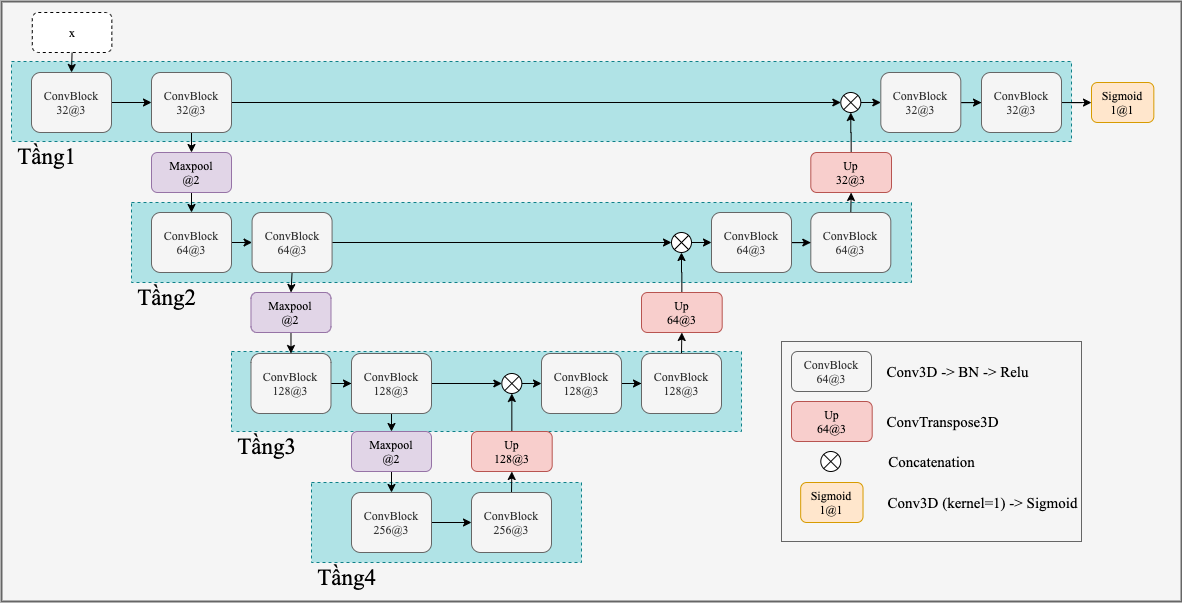
\includegraphics[width=14cm]{images/blood/model-Unet3D.png}
    \caption{Mô hình Unet3D 4 tầng}
    \label{unet3d_arch}
\end{figure}

Về mặt tổng quan kiến trúc này không khác nhiều so với kiến trúc mô hình Unet2D, tuy nhiên để ứng dụng vào các bài toán cụ thể khác nhau, chúng ta cần sử dụng các siêu tham số như số tầng phù hợp bởi kích thước các đối tượng của bài toán. Đối với những đối tượng bài toán rất nhỏ như mạch máu, việc mô hình càng sâu đặc trưng thu được sẽ càng có tính toàn cục điều này khiến cho các vùng chứa mạch máu có thể bị phá vỡ.\par


\section{Mô hình TLUnet3D} \label{bg-TLUnet3D}
Mô hình TLUnet3D được giới thiệu trong \cite{LV_LIVER} là một biến thể của mô hình Unet3D sử dụng phương pháp học chuyển tiếp (transfer learning) để cải thiện kết quả phân đoạn. Đây là phương pháp sử dụng lại trọng số của một số lớp, hoặc toàn bộ các lớp của một mô hình đã được huấn luyện trước đó để khởi tạo cho các lớp trên mô hình mới.\par
Mô hình TLUnet3D gồm ba phần: mã hóa, giải mã và nối tắt. Phần mã hóa sử dụng lại kiến trúc và trọng số của mô hình tích chập 3 chiều (CNN3D) hay nói cách khác, mô hình CNN3D cần được huấn luyện trước mô hình TLUnet3D. Kiến trúc mô hình CNN3D như sau:
\begin{figure}[H]
    \centering
    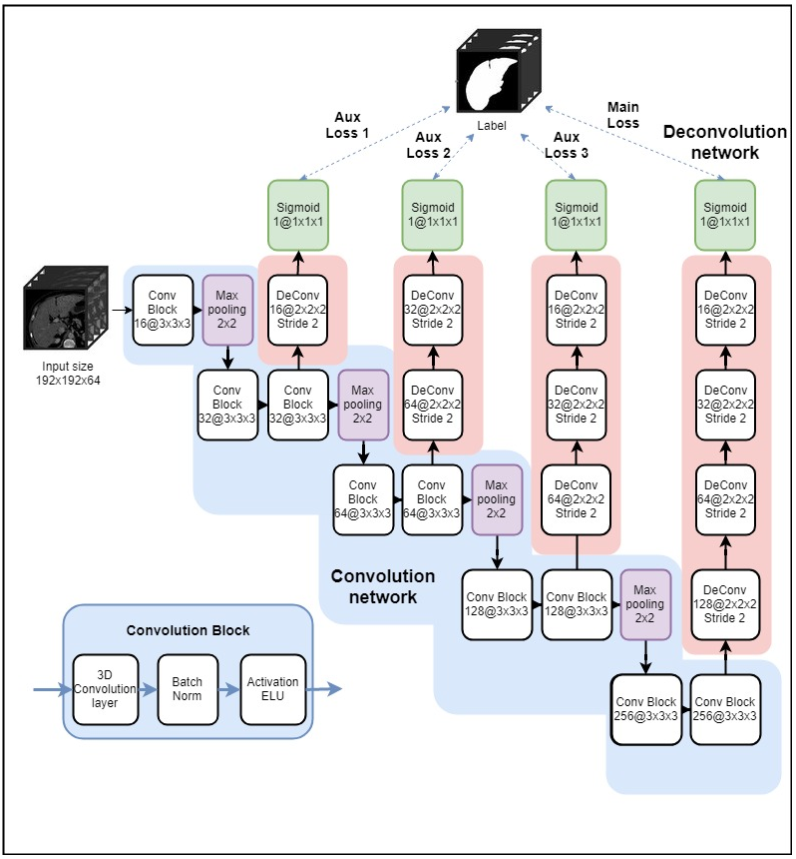
\includegraphics[width=12cm]{images/liver/CNN3D/CNN3D.png}
    \caption{Kiến trúc mô hình CNN3D\cite{LV_LIVER}}
    \label{fig:CNN3D}
\end{figure}
Hàm mất mát của mô hình CNN3D được tính từ hàm mất mát của tất cả các phần giải mã:
\begin{align}
    \label{LossCNN3D}
    Loss = \mu_{1}Loss_{aux1} + \mu_{2}Loss_{aux2} + \mu_{3}Loss_{aux3} + \mu_{4}Loss_{main}
\end{align}
\textbf{Cơ chế giám sát sâu (Deep supervision)} được đề xuất năm 2016 \cite{Deepsupervision} bởi Qi Dou và cộng sự đã được tác giả kế thừa trong quá trình huấn luyện mô hình CNN3D. Cơ chế giám sát sâu giúp mô hình học tập hiệu quả và đem lại kết quả tốt hơn so với phương pháp học thông thường. Thông qua việc sử dụng thêm các cổng ra tại từng tầng của giai đoạn mã hóa, trọng số của các lớp tính toán sẽ được cập nhập và chia sẻ thông tin với nhau giữa các luồn thay vì chỉ chạy xuyên qua 1 luồn chính như mô hình gốc Unet. Nhờ vào đó, đặc trưng trích xuất qua từng tầng của giai đoạn mã hóa sẽ trở nên trừu tượng có ích hơn vì chúng được kiểm tra song song với giá trị cuối cùng. Về hàm lỗi, tác giả đã sử dụng hàm Binary Cross-Entropy để huấn luyện mô hình với các siêu tham số $\mu_{1} = 1$,  $\mu_{2} = 2$,  $\mu_{3} = 4$,  $\mu_{4} = 8$. 

Khác biệt thứ 2 là ở phần nối tắt của mô hình TLUnet3D, tác giả đã thêm một lớp tích chập với kích thước cửa sổ 5x5 vào phần nối tắt để giảm số kênh (channel) trước khi kết hợp với kết quả lớp đảo tích chập tương ứng. Phần giải mã tương tự như phần giải mã của mô hình Unet3D nhưng được chỉnh sửa số lượng kênh.

Khi huấn luyện mô hình TLUnet3D, chỉ có phần giải mã và nối tắt được huấn luyện, trọng số của phần mã hóa được đóng băng. Mô hình được huấn luyện với số lượng dữ liệu ít hơn lúc huấn luyện mô hình CNN3D để tránh xảy ra hiện tượng quá khớp (overfitting). Kiến trúc mô hình cụ thể tại Hình \ref{tlunet}.

Ở bước tiền xử lý dữ liệu, tác giả sử dụng công cụ Anisotropic diffusion filter trong thư viện SimpleItk để loại bỏ nhiễu. Việc này mất khá nhiều thời gian nhưng đem lại kết quả tốt.

Kỹ thuật hậu xử lý tìm thành phần liên thông lớn nhất (gan) sau đó loại bỏ các thành phần còn lại (loại bỏ khối) cùng với kỹ thuật lấp đầy khối cũng được tác giả sử dụng. Việc áp dụng hậu xử lý giúp cải thiện kết quả phân đoạn gan.

\begin{figure}[H]
    \centering
    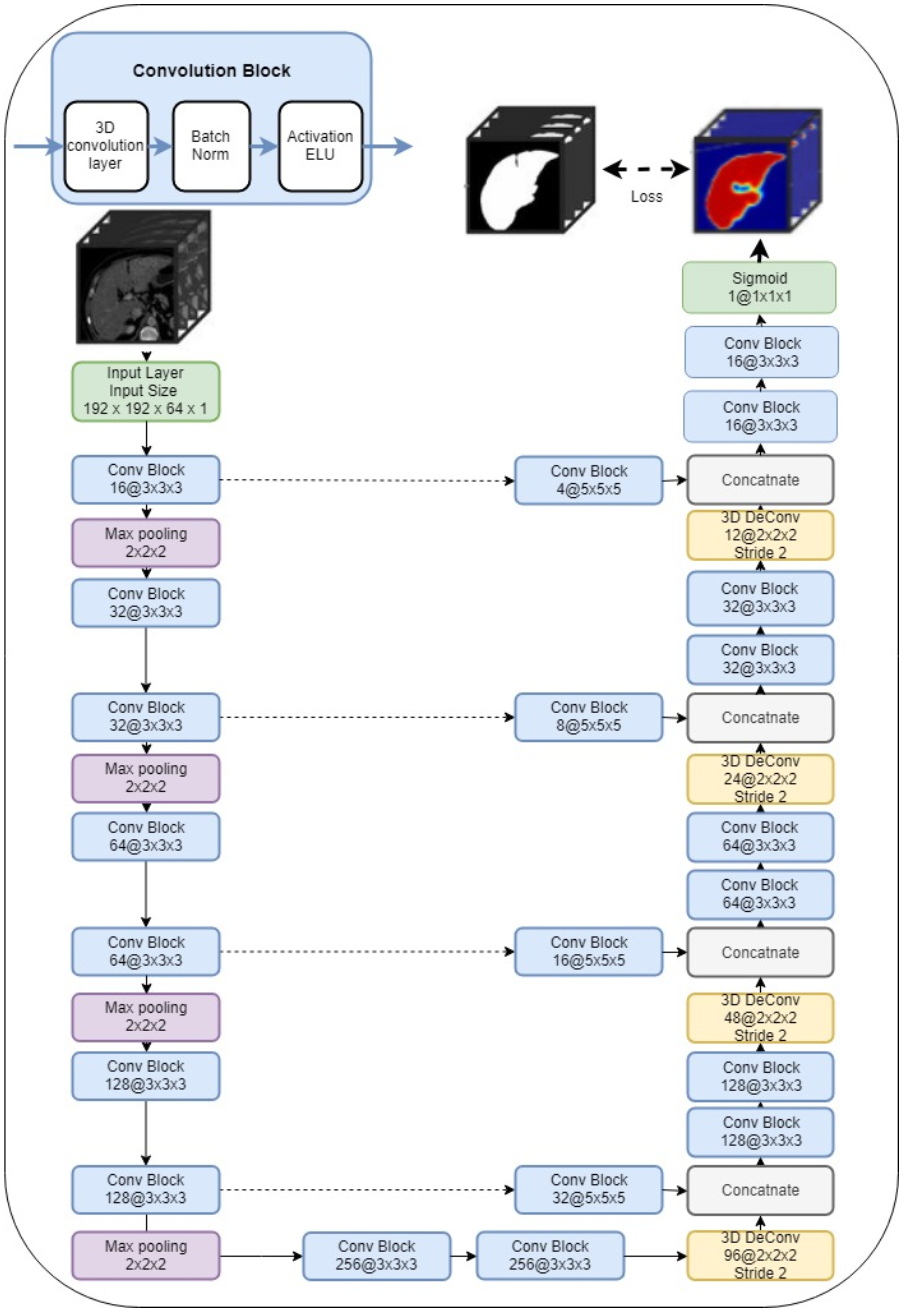
\includegraphics[width=14cm]{images/liver/TLUnet3D/TLUnet3D.png}
    \caption{Kiến trúc mô hình TLUnet3D\cite{LV_LIVER}}
    \label{tlunet}
\end{figure}

\begin{figure}[H]
    \centering
    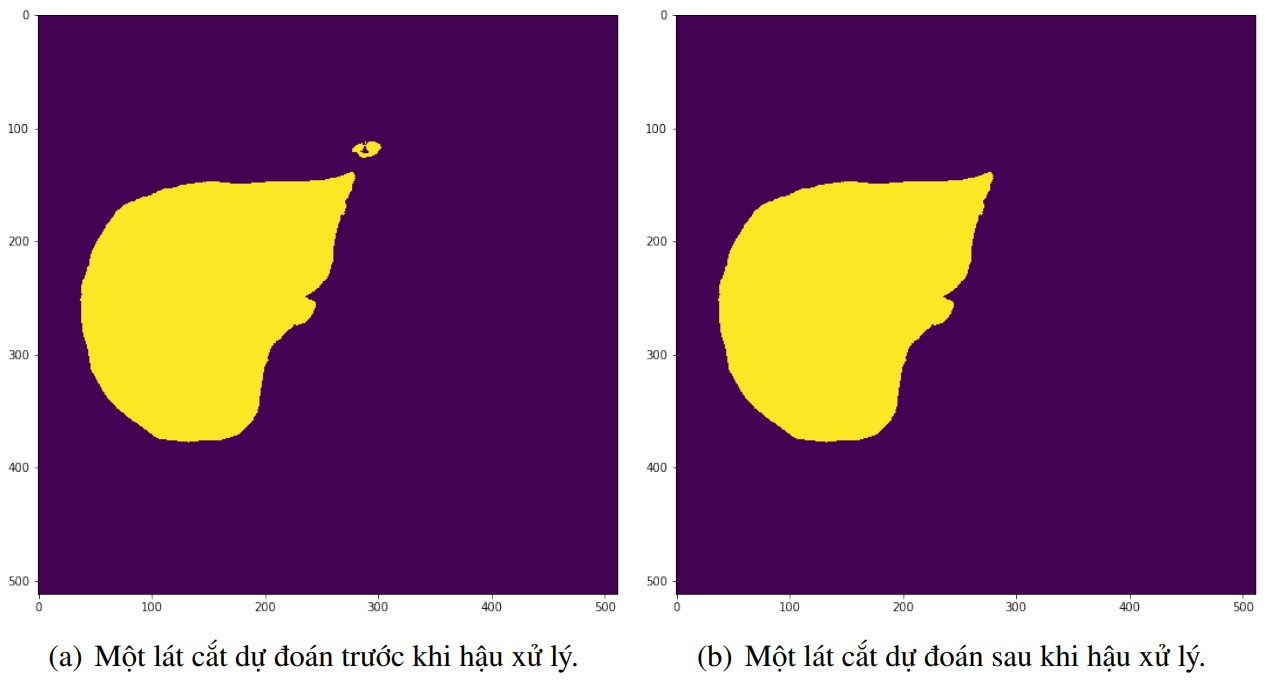
\includegraphics[width=12cm]{images/liver/TLUnet3D/posprocessing.jpg}
    \caption{Thay đổi của một dự đoán trước và sau hậu xử lý \cite{LV_LIVER}}
    \label{posprocessing}
\end{figure}
\vspace{-5mm}
Thực tế, mô hình CNN3D được huấn luyện trên ba tập dữ liệu Sliver07, Lits17 và 3Dircadb đã đem lại kết quả tốt, mô hình TLUnet3D giúp làm mượt (fine-tune) trên từng tập để cải thiện kết quả trên từng tập dữ liệu tương ứng. Mô hình TLUnet3D cho kết quả Dice cải thiện khoảng 1\% trên từng tập so với mô hình CNN3D theo công bố của tác giả. 

\newpage

\section{Mô hình U\textsuperscript{2}net}
Mô hình mạng U\textsuperscript{2}net được giới thiệu trong bài báo \cite{u2-net} bởi Qin và cộng sự vào năm 2020. Bài toán mà tác giả hướng đến là phát hiện đối tượng nổi bật nhất trong ảnh (Salient object detection - SOD). Tuy đây không phải là bài toán phân đoạn ảnh y khoa nhưng về phương pháp đều là gắn nhãn cho từng điểm ảnh thuộc đối tượng nổi bật (foreground) hoặc là nền (background). Điều này khá tương đồng với bài toán phân đoạn, và mô hình này đã đạt được kết quả cao nhất trong các mô hình hiện đại (state of the art) trong lĩnh vực SOD với chỉ số $F_{measure}$ đạt trên 95\% (Hình \ref{BenU2net}). Thứ hai, mô hình mà tác giả sử dụng là biến thể của mạng Unet (mô hình backbone được nhóm tập trung cải thiện), do đó đây là bài báo đáng được tham khảo.

\begin{figure}[H]
	\begin{center}
		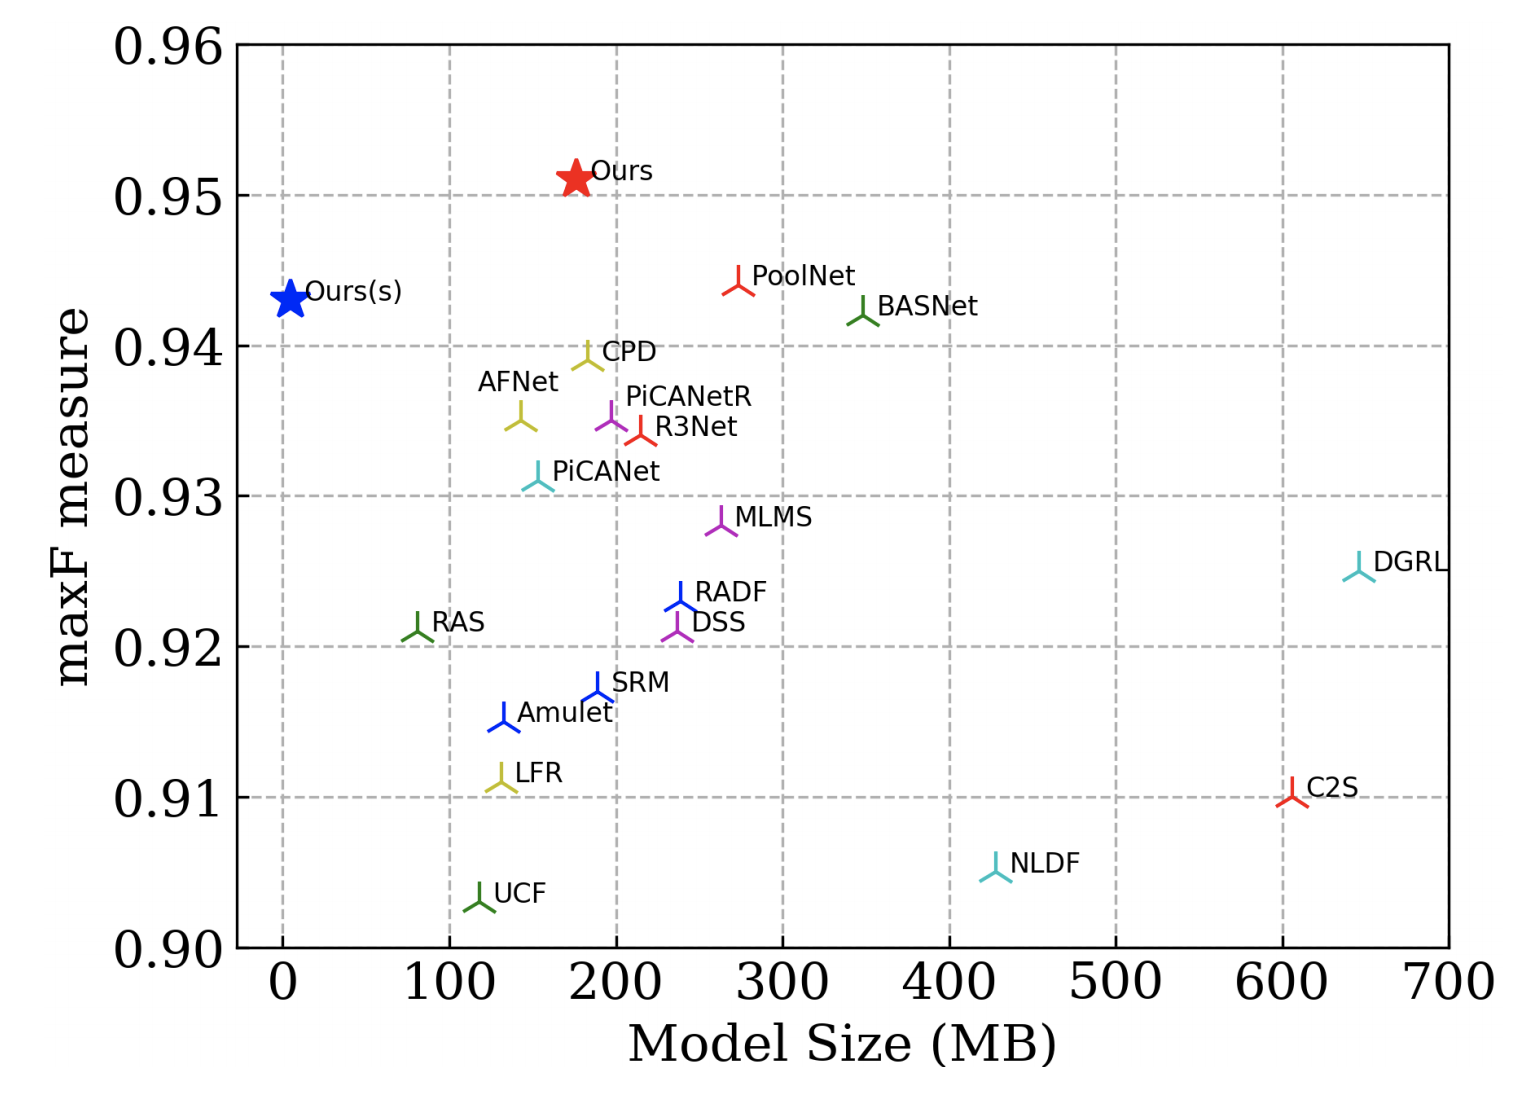
\includegraphics[width=8cm]{images/blood/u2_benk.png}
		\caption{So sánh mức độ hiệu quả U2net và các mô hình các trong lĩnh vực SOD\cite{u2-net}.}
		\label{BenU2net}
	\end{center}
\end{figure}
\vspace{-1.0cm}

\subsection{Hướng tiếp cận}
Bất lợi của các mô hình phân đoạn hiện nay, các đặc trưng mang thông tin toàn cục nhiều sẽ được mô hình trích xuất ở các lớp sâu hơn (thông thường sẽ qua các lớp gộp để giảm chi phí tính toán). Do đó khi chạy qua các lớp sâu thường sẽ khiến kích thước các đặc trưng giảm dần qua từng tầng và chúng mới mang lại nhiều thông tin ngữ cảnh toàn cục. Trong khi đó việc các đặc trưng mang tính ngữ cảnh toàn cục hay cục bộ đều rất quan trọng trong việc dự đoán điểm ảnh đó có thuộc đối tượng cần dự đoán hay không bởi các đối tượng có nhiều kích thước khác nhau. Với bất lợi đó nên các mô hình hiện tại chỉ đi sâu với một số tầng nhất định. Để giải quyết bất lợi đó, tác giả đã đề xuất một kiến trúc khối giúp cho việc có thể cho các đặc trưng đi sâu hơn qua các lớp mà vẫn giữ được kích thước đặc trưng ban đầu của chúng đó là khối Residual U-block.

\subsection{Khối Residual U-block - RSU}
Sự khác biệt đầu tiên giữa khối RSU với các khối tích chập thông thường là nhánh kết nối tắt, tác giả đã có sự cải tiến so với phép lấy phần dư được giới thiệu trong mạng phần dư (ResNet) \cite{resnet} được giới thiệu năm 2015. Thay vì sử dụng lại giá trị đầu vào ban đầu, tác giả đã sử dụng một tầng tích chập để trích xuất các đặc trưng cục bộ, rồi truyền nó thông qua phép nối tắt xuyên qua một hay nhiều lớp như hình \ref{RSB}.b.

\begin{figure}[H]
	\begin{center}
		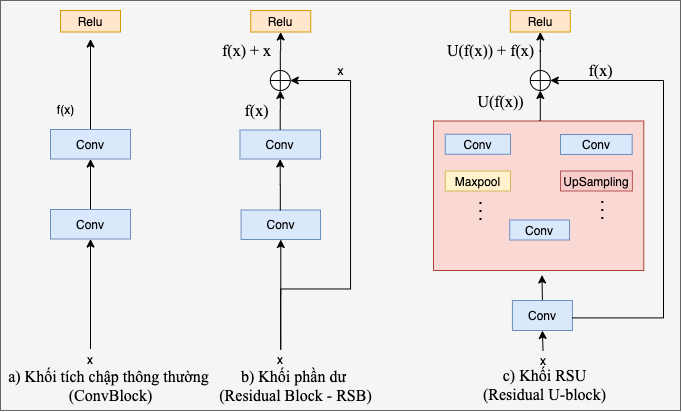
\includegraphics[width=10cm]{images/blood/compareRSU.png}
		\caption{So sánh giữa khối Residual U-Block(RSU) và  các khối tích chập phổ biến. }
		\label{RSB}
	\end{center}
\end{figure}
\vspace{-1.0cm}
Thứ hai, lấy ý tưởng từ mô hình Unet \cite{Unet}, một kiến trúc chữ gồm 2 phần: phần mã hóa và phần giải mã, đặc trưng đầu vào sẽ được mã hóa thông qua nhiều tầng khác nhau sau đó được giải mã về kích thước ban đầu. Nhờ vào đó đặc trưng được trích xuất từ khối tính toán này sẽ mang nhiều thông tin ngữ cảnh toàn cục hơn so với khối tích chập thông thường, bởi việc nó trích xuất thông tin dựa trên những kích thước khác nhau qua từng tầng trích xuất. Sau đó được giải mã về kích thước ban đầu, điều này giúp cho các đặc trưng sau khi qua khối RSU sẽ còn có kích thước đủ lớn để đi sâu thêm những tầng về sau.

Tổng hợp 2 ý tưởng, khối RSU sẽ đem lại vừa là thông tin toàn cục (bởi việc đi sâu xuống tầng mã hóa) vừa là thông tin cục bộ (nhờ vào tầng tích chập đầu tiên) được kết hợp lạị với nhau. Kiến trúc khối U-Block được trình bày như hình \ref{rsu}.

\begin{figure}[H]
	\begin{center}
		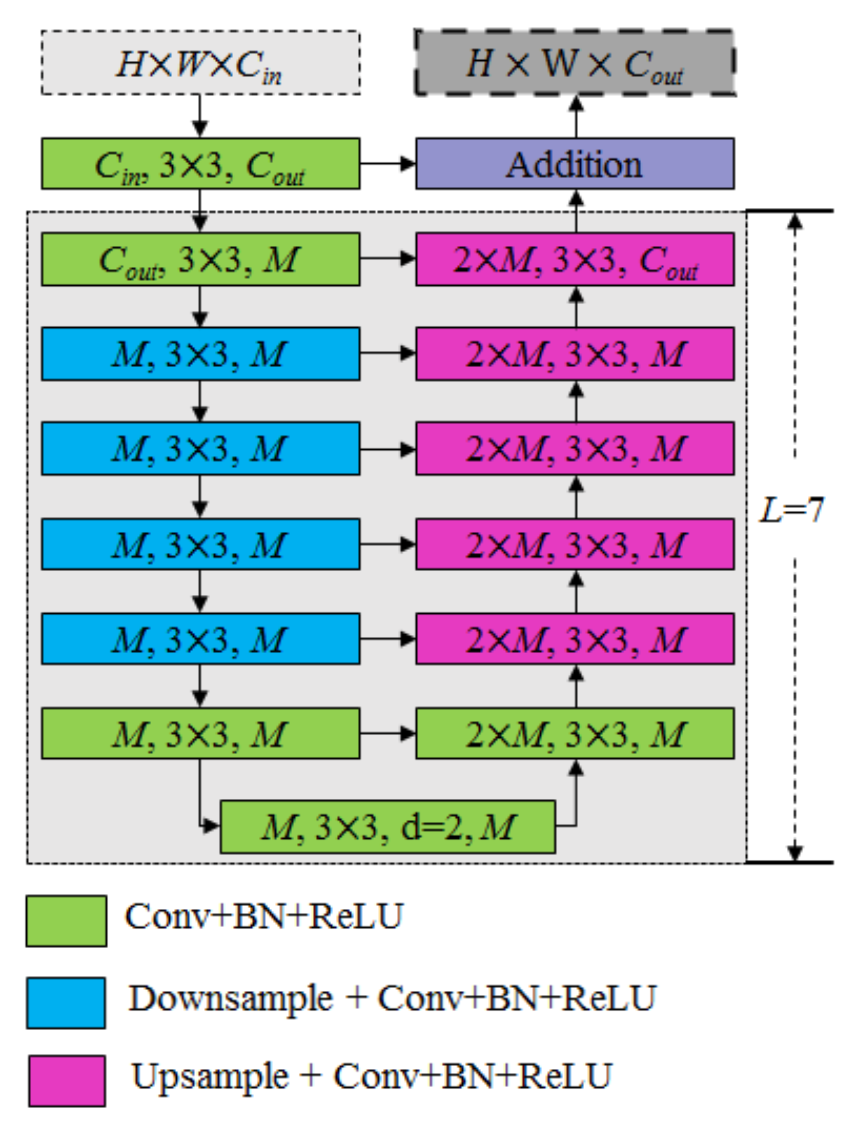
\includegraphics[width=8cm]{images/blood/RSU.png}
		\caption{Kiến trúc khối Residual U-block (RSU)\cite{u2-net}. }
		\label{rsu}
	\end{center}
\end{figure}
\vspace{-1.0cm}

Một khối RSU sẽ có 3 siêu tham số: $\mathrm{C_{in}, C_{out}, L}$ tương ứng với số kênh đầu vào/đầu ra và độ sâu của mạng. Một khối có kiến trúc đối xứng giữa phần mã hóa và phần giải mã với độ sâu L với mục tiêu trích xuất thông tin ngữ cảnh thông qua từng kích thước đặc trưng khác nhau (multi-scale contextual information) được ký hiệu U(F(x)). Với F(x) là đặc trưng cục bộ được trích xuất đầu tiên nhờ vào tầng tích chập. Độ sâu L càng lớn, càng nhiều phép gộp được sử dụng nhờ đó tăng vùng nơron nhìn thấy (receptive field) giúp làm giàu thông tin ngữ cảnh toàn cục hơn. Ký hiệu M là siêu tham số của khối RSU, đại diện số lượng các đặc trưng được trích xuất qua mỗi tầng tích chập.

\subsection{Kiến trúc mạng}
Kiến trúc mạng U\textsuperscript{2}net sẽ có kiến trúc tổng quan giống như mạng Unet bao gồm 2 nhánh: nhánh mã hóa và nhánh giải mã.

\begin{figure}[H]
	\begin{center}
		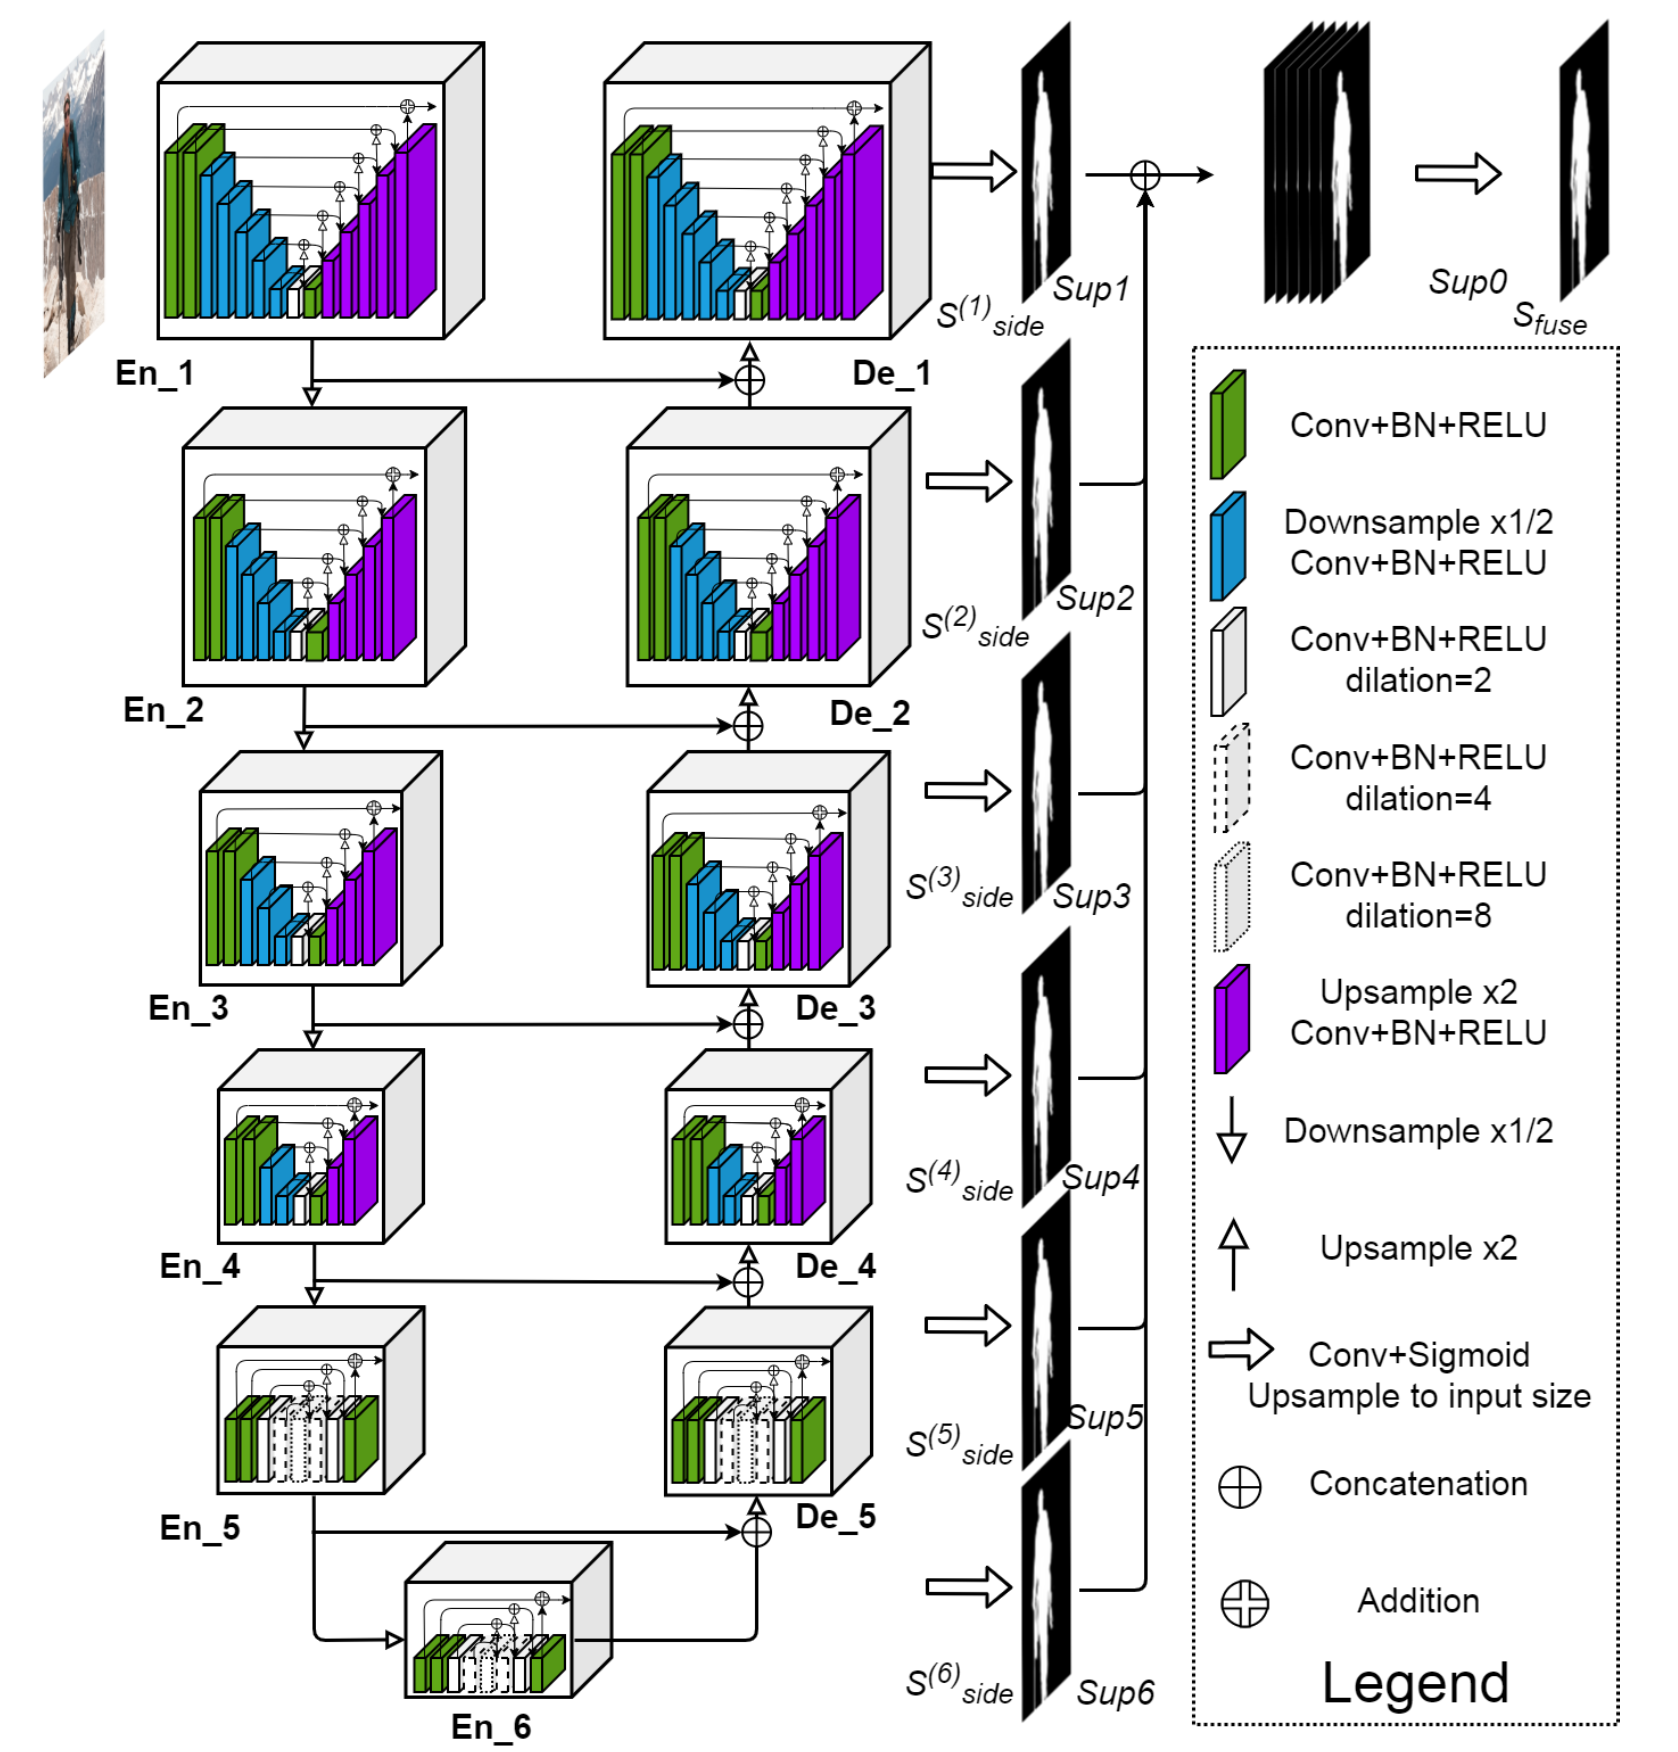
\includegraphics[width=12cm]{images/blood/u2net_paper.png}
		\caption{Kiến trúc mô hình U\textsuperscript{2}net\cite{u2-net}. }
		\label{u2net_arch}
	\end{center}
\end{figure}
\vspace{-1.0cm}

Thay bằng việc sử dụng các khối tích chập thông thường tác giả đã sử dụng khối Residual U-block được giới thiệu ở trên để tạo thành bộ mã hóa và giải mã tương ứng. Mô hình có độ sâu là 6: gồm 6 tầng tương ứng với 5 phép gộp đối xứng với 5 phép upsample (không có trọng số). Qua mỗi tầng kích thước các đặc trưng thu được sẽ giảm đi một nữa. Tại mỗi tầng sẽ bao gồm 2 khối RSU (1 khối tại phần mã hóa, 1 khối tại phần giải mã). Mỗi khối RSU sẽ có độ sâu là L. Tương ứng với mỗi tầng độ sâu khối L sẽ có giá trị giảm dần 1 đơn vị, tại tầng đầu tiên (En\_1) khối RSU sẽ có L=7, tại tầng thứ 2 sẽ có L=6 cho đến tầng cuối cùng. Mô hình có sử dụng phép kết nối tắt (skip connection) giữa bộ mã hóa (encoder) và bộ giải mã (decoder) với mục tiêu trong quá trình khôi phục kích thước tại mỗi tầng, đặc trưng sẽ được kết hợp với thông tin mã hóa ban đầu nhằm tăng tính ngữ cảnh . Bên cạnh đó việc sử dụng các phép kết nối tắt giúp cho mô hình tránh tình trạng đạo hàm bị tiêu biến (Vanishing Gradient).

    \chapter{TẬP DỮ LIỆU}

\section{Khảo sát dữ liệu}
Như đã đề cập ở Chương \ref{chapter:introduction}, không có nhiều tập dữ liệu được gắn nhãn về gan và mạch máu được công khai. Sau đây là một số tập dữ liệu phổ biến sẽ được dùng để nghiên cứu.
Mô hình phân đoạn gan sẽ sử dụng cả 3 tập dữ liệu được đề cập. Mô hình phân đoạn mạch máu sẽ chỉ dùng tập dữ liệu 3DIRCAD (vì hiện tại chỉ có tập dữ liệu này được gán nhãn mạch máu được công bố).

\subsection{Liver Tumor Segmentation Challenge 2017}
\textbf{Liver Tumor Segmentation Challenge (LITS2017)}\cite{lits}: là tập dữ liệu được sử dụng trong cuộc thi phân đoạn gan và khối u gan do ISBI và MICCAI hợp tác tổ chức vào năm 2017. Tập dữ liệu bao gồm 131 ảnh CT có gắn nhãn dùng để huấn luyện và 70 ảnh CT chưa có nhãn dùng để đánh giá. Bộ dữ liệu được thu thập bởi các máy quét và giao thức khác nhau từ sáu vị trí lâm sàng khác nhau, với độ phân giải trong mặt phẳng thay đổi lớn từ 0,55 mm đến 1,0 mm và khoảng cách lát từ 0,45 mm đến 6,0 mm.\par

 Dữ liệu gồm các file \textit{volume} được đánh số từ 0 đến 130 là ảnh CT, cùng với đó là các file \textit{segmentation} là nhãn tương ứng cũng được đánh số từ 0 đến 130. Tất cả các file đều ở định dạnh 'nii'. Trong đó có 118 ảnh chứa khối u trên tổng số 131 bộ ảnh CT.

\begin{figure}[H]
    \centering
    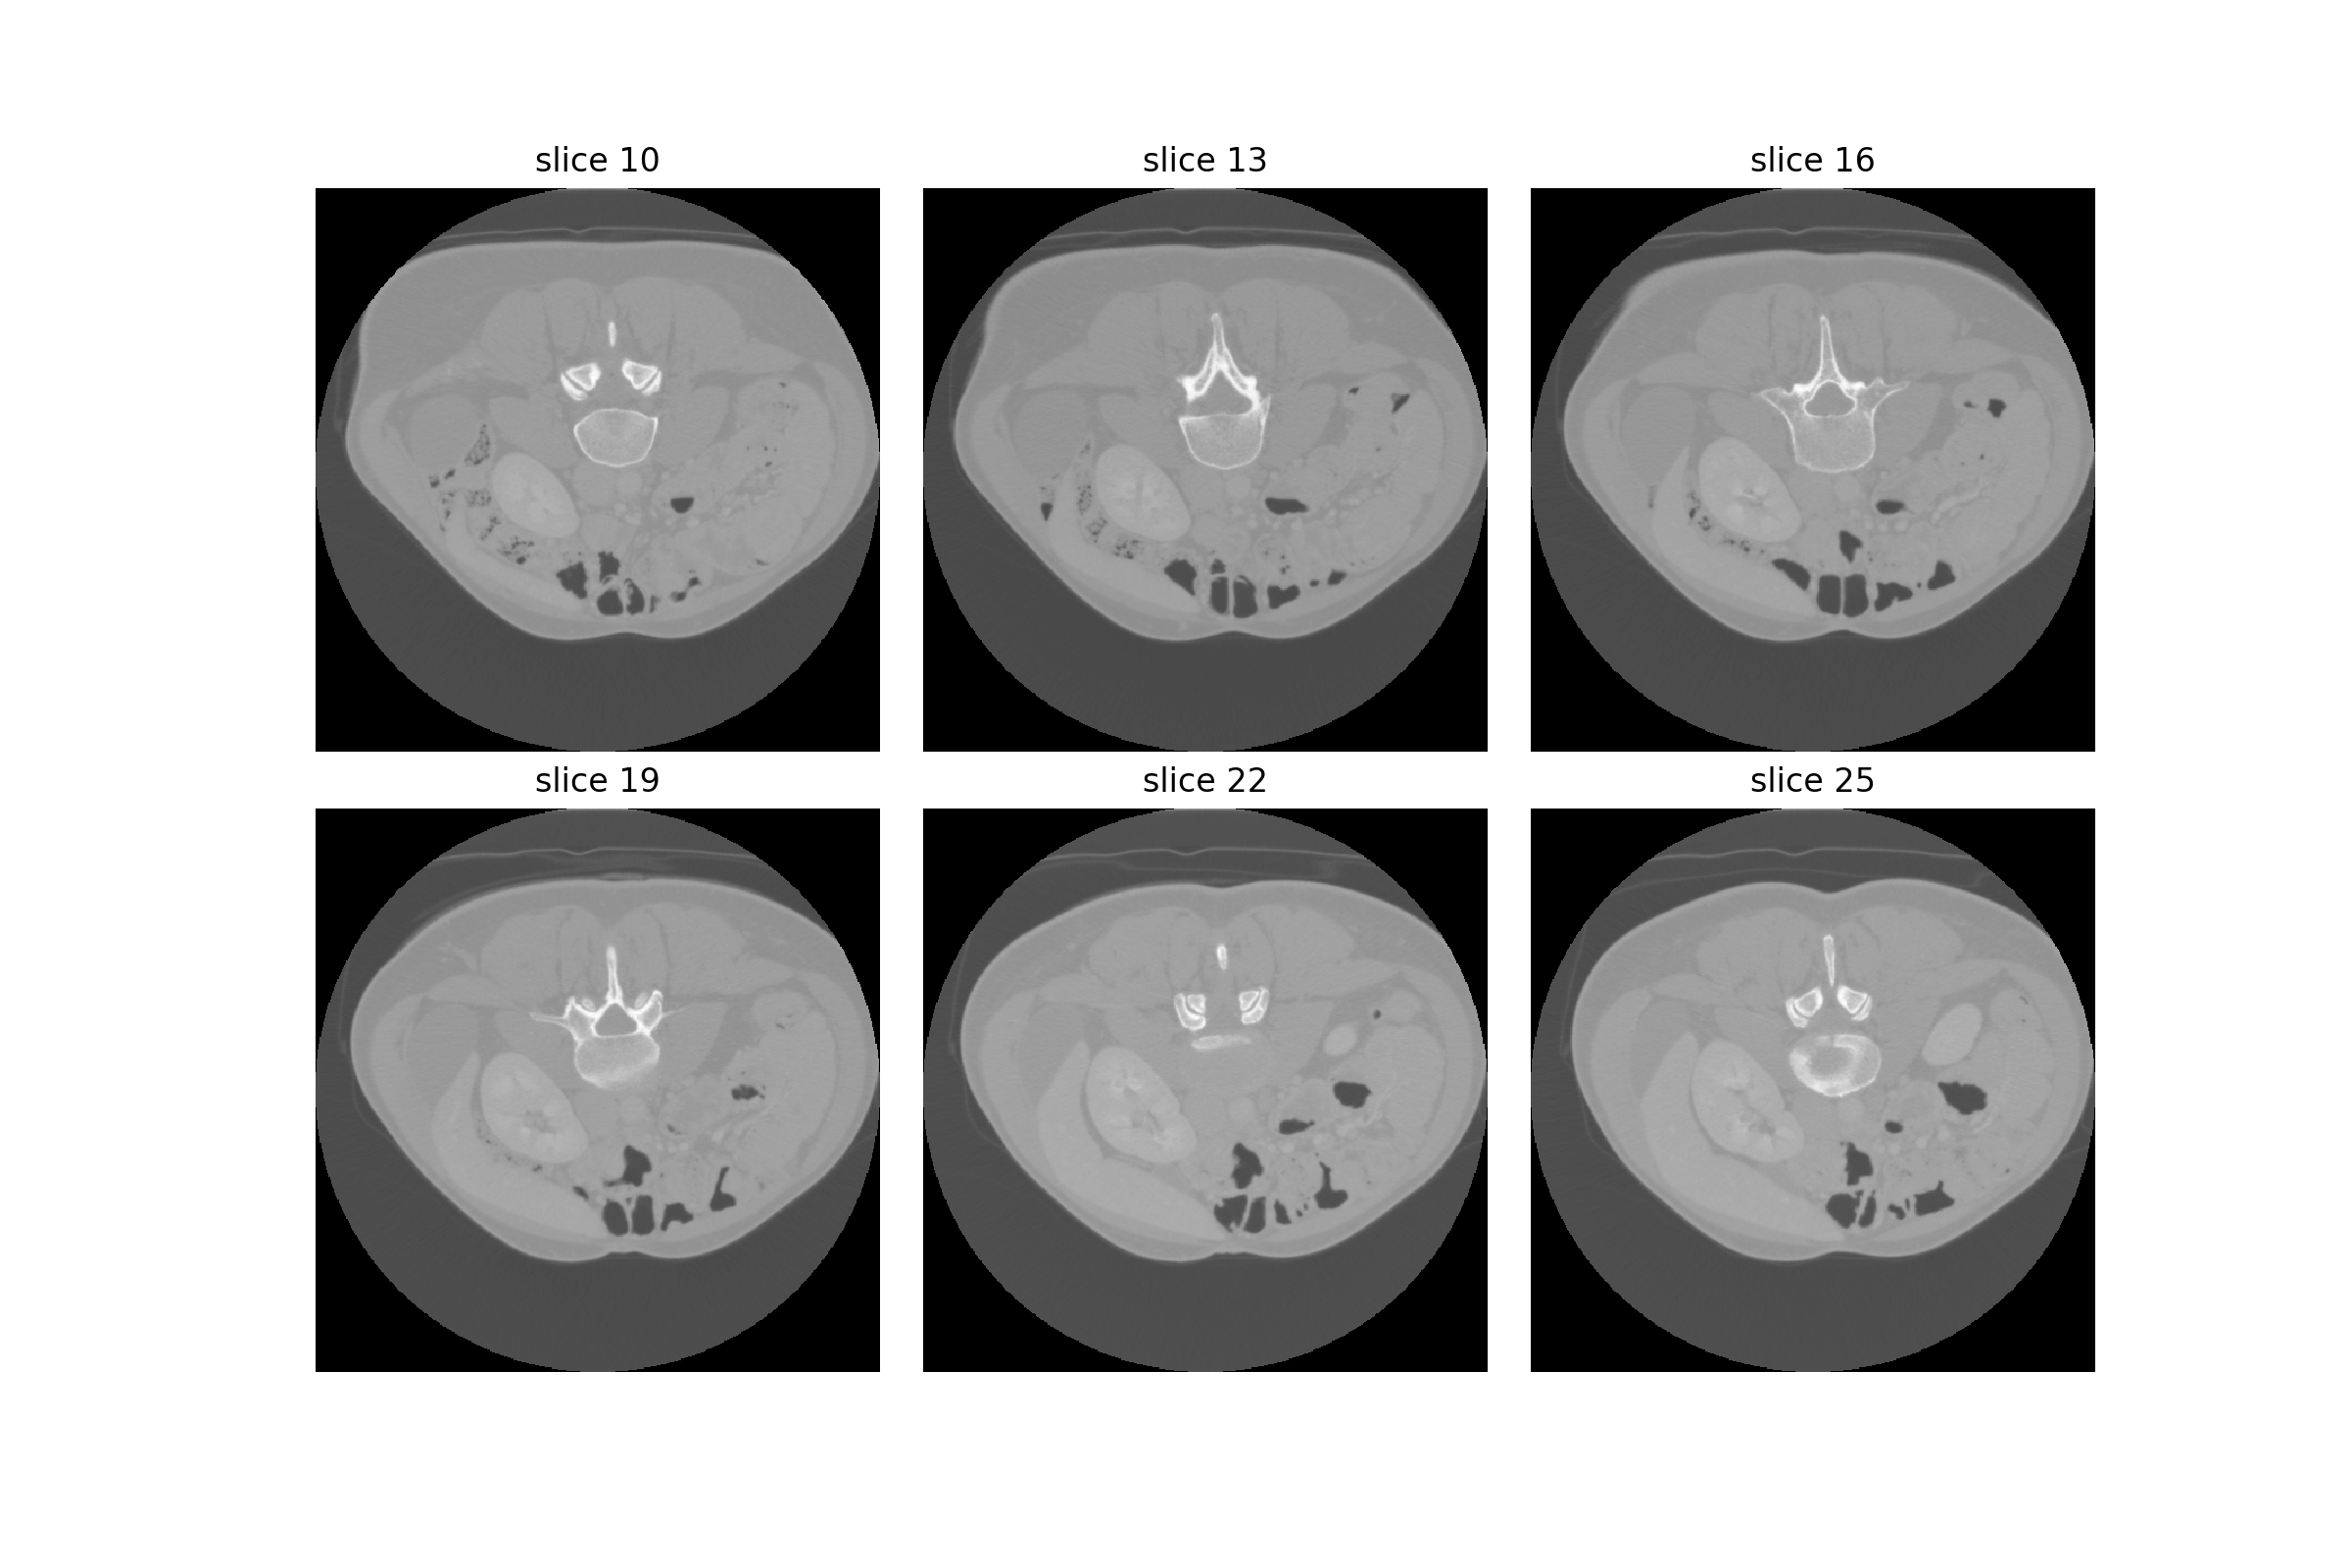
\includegraphics[width=10cm]{images/experience/volume-35-6slice.png}
    \caption{Một vài lát cắt trong ảnh volume-35 lấy từ tập dữ liệu LITS2017.}
\end{figure}
Tất cả các lát cắt đều có kích thước $512\times 512$ nhưng số lượng mỗi lát cắt trong mỗi ảnh CT là khác nhau. Cụ thể tính trên 130 ảnh huấn luyện, số lát cắt nhỏ nhất là 74, lớn nhất là 987 và trung bình là 448.\par
Như đã đề cập, dữ liệu bị mất cân bằng nghiêm trọng giữa phần nền và phần gan. 

\begin{figure}[H]
  \centering
  \subfloat[Tỉ lệ thể tích của gan đối với nền]{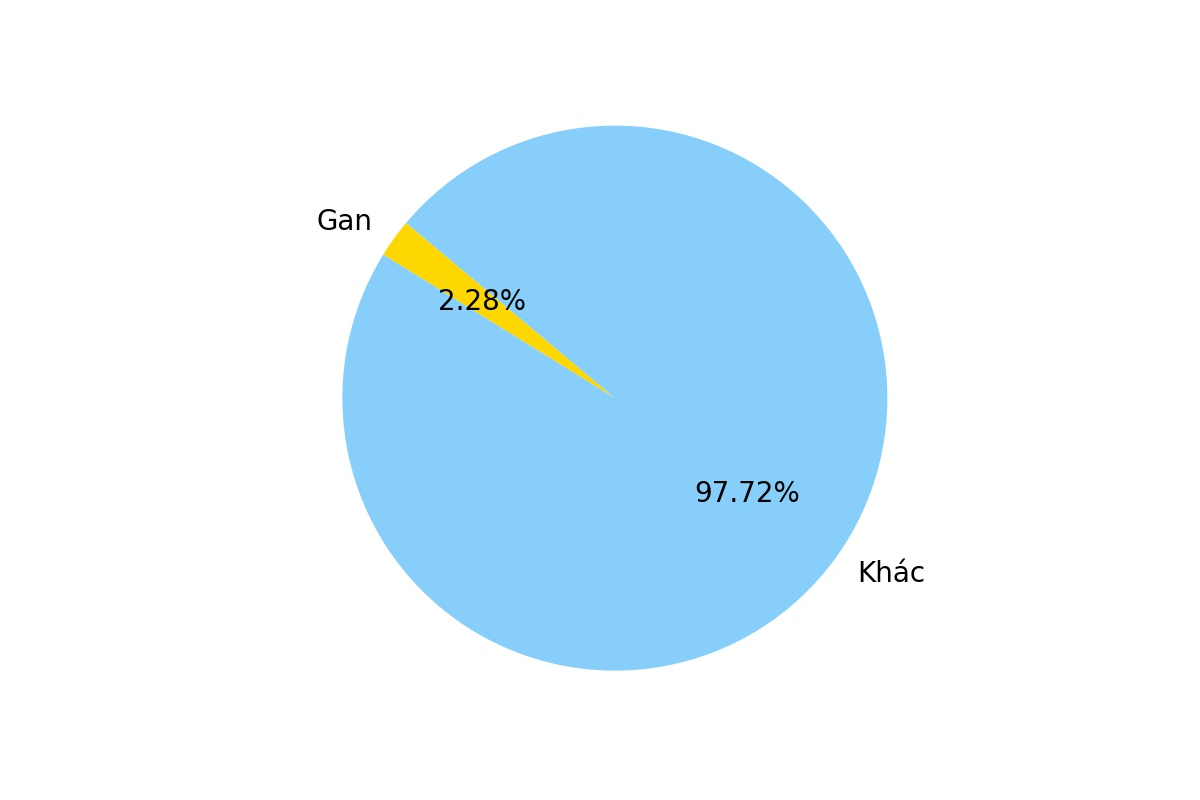
\includegraphics[width=0.45\textwidth]{images/experience/liver_background.jpg}\label{fig:f1}}
  \hfill
  \subfloat[Tỉ lệ thể tích của khối u so với gan]{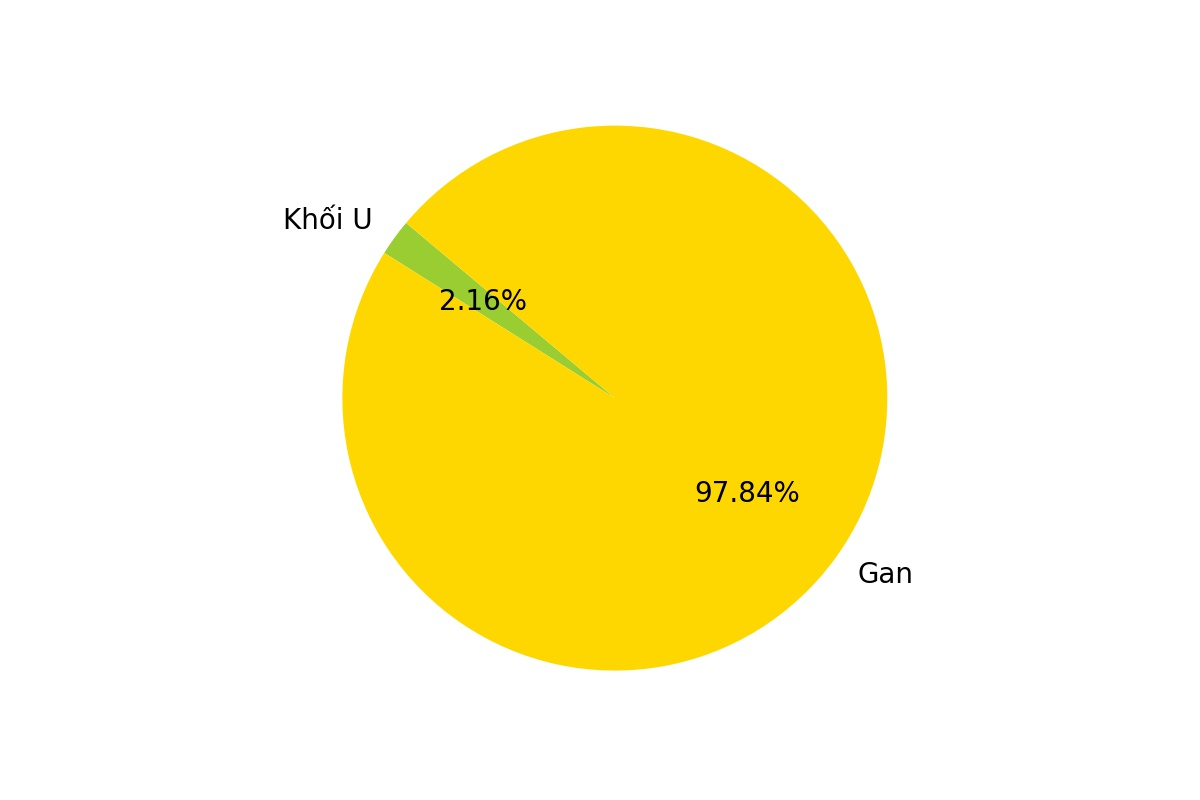
\includegraphics[width=0.45\textwidth]{images/experience/tumor_liver.jpg}\label{fig:f2}}
  \caption{Tỉ lệ thể tích của gan, khối u và nền trên tập huấn luyện LITS2017.}
\end{figure}

Qua biểu đồ, ta thấy rằng thể tích gan chỉ chiếm 2.28\% trong khi phần nền chiếm tới 97.72\%, u chỉ chiếm hơn 2\% trên tổng thể tích của gan, đặc biệt khi xem xét đến tỉ lệ thể tích của khối u so với nền, đây thực sự là một thách thức lớn.\par

\subsection{Segmentation of the Liver 2007}
\textbf{Segmentation of the Liver 2007 (SLIVER07)} \cite{sliver07}: Đây là tập dữ liệu được sử dụng trong
một cuộc thi thuộc khuôn khổ hội nghị MICCAI 2007 dành cho các hệ thống \textit{phân đoạn
lá gan} tự động và bán tự động. Trong đó gồm 20 ảnh CT có gắn nhãn phục vụ mục đích huấn luyện và 10 ảnh CT không nhãn để chấm điểm online. Số mặt cắt trong tập ảnh nằm trong khoảng từ 64 đến 388
ảnh 2-chiều. Khoảng cách mỗi điểm ảnh trong mỗi ảnh cắt ngang nằm trong khoảng 0.55
đến 0.8 mi-li-mét, khoảng cách hai mặt cắt liên tiếp từ 1 đến 3 mi-li-mét. Mỗi ảnh CT
đều đi kèm với các thông số trên. 

\subsection{3Dircadb}
\textbf{3D Image Reconstruction for Comparison of Algorithm Database (3Dircadb)} \cite{3dircad}: Đây là tập dữ liệu do Viện nghiên cứu chống ung thư đường tiêu hóa của trường Đại học Bệnh viện IRCAD tại Pháp cung cấp. Đây là tập dữ liệu chứa thông tin gần như đầy đủ các cơ quan trong lồng ngực gồm: phổi, gan, xương, động/tĩnh mạch, thận, khối u gan... Do đó việc huấn luyện mô hình phân đoạn mạch máu sẽ tập trung vào tập dữ liệu này. \par

3D-IRCADb có hai gói dữ liệu là 3D-IRCADb-01 và 3D-IRCADb-02. Chúng tôi chọn sử dụng gói 3D-IRCADb-01 tiến hành huấn luyện và đánh giá hệ thống phân đoạn trong luận văn này. Tập dữ liệu này cung cấp một số bộ ảnh y khoa từ các bệnh nhân được ẩn danh bao gồm 20 ảnh CT lồng ngực của 20 bệnh nhân (10 nam - 10 nữ) và các cơ quan của từng bệnh nhân được gán nhãn bằng phương pháp thủ công bởi các chuyên gia lâm sàng. \par

 3D-IRCADb-01 bao gồm các bộ ảnh CT với sự xuất hiện của khối u gan trong 75\% các trường hợp. Hệ thống mạch máu trong các bộ ảnh CT được chia thành ba phần là \textit{tĩnh mạch chủ}, \textit{tĩnh mạch cửa} và \textit{động mạch} và được phân đoạn riêng cho từng loại mạch máu. Số mặt cắt trong tập ảnh nằm trong khoảng từ 91 đến 260 ảnh 2-chiều. Các ảnh trong tập dữ liệu này có các khoảng cách giữa các điểm ảnh từ 0,56mm đến 0,81mm, khoảng cách hai mặt cắt từ 1,6mm đến 4mm. Hình \ref{3dircad_sample} là ảnh trực quan dữ liệu cho từng bệnh nhân trong gói 3D-IRCADb-01. 

\begin{figure}[H]
    \centering
    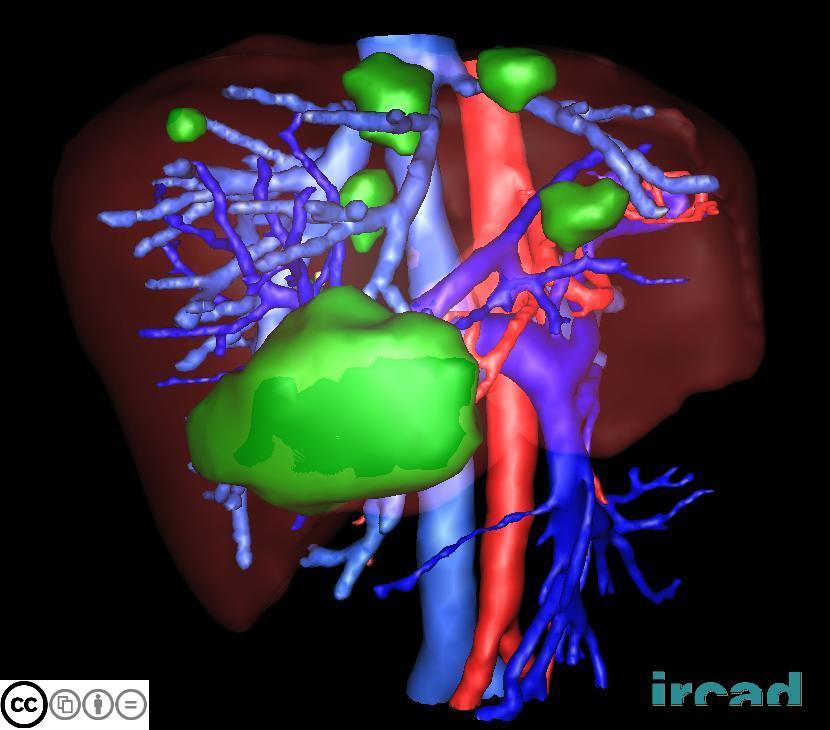
\includegraphics[width=8cm]{images/dataset/3Dircadb1.jpg}
    \caption{Ảnh trực quan các bộ phân được đánh nhãn trong tập dữ liệu \cite{3dircad}.}
    \label{3dircad_sample}
\end{figure}
\vspace{-10mm}

\section{Tiền xử lý dữ liệu}
\subsection{Chuẩn bị dữ liệu} \label{data-preparation}
Đối với các giải thuật học máy hiện nay, khâu chuẩn bị dữ liệu là vô cùng quan trọng. Cụ thể hơn học sâu là một phần của một họ các phương pháp học máy rộng hơn dựa trên đại diện học của một tập dữ liệu. Do đó nếu chúng ta sử dụng một mô hình được học trên tập dữ liệu có phân bố khác với tập kiểm tra thì kết quả dự đoán của mô hình không thể đạt được sự chính xác như ta kì vọng. Do đó ta cần phải có 1 khảo sát để xác định một phương pháp chia dữ liệu thích hợp.\par

Đầu tiên, trong tập 3DIRCAD gồm 20 bệnh nhân, chúng tôi tiến hành khảo sát mức độ phân bố giá trị Hounsfield Unit (của gan và máu tương ứng). \textit{Hình} \ref{hu_dist} được vẽ dựa trên giá trị trung bình (mean) và 2 lần giá trị độ lệch chuẩn (std) thể hiện 95\% giá trị HU của mạch máu (gan) phân phối trong khoảng giá trị đó. Dựa vào bệnh nhân số 8 và bệnh nhân số 9 ta có thể thấy được sự khác biệt trong phân bố giá trị HU ở cả gan và mạch máu (ở gan, bệnh nhân 8 phân bố quanh giá trị 160 trong khi đó bệnh nhân số 9 phân bố quanh giá trị 80 
đối với gan).

\begin{figure}[H]
	\begin{center}
		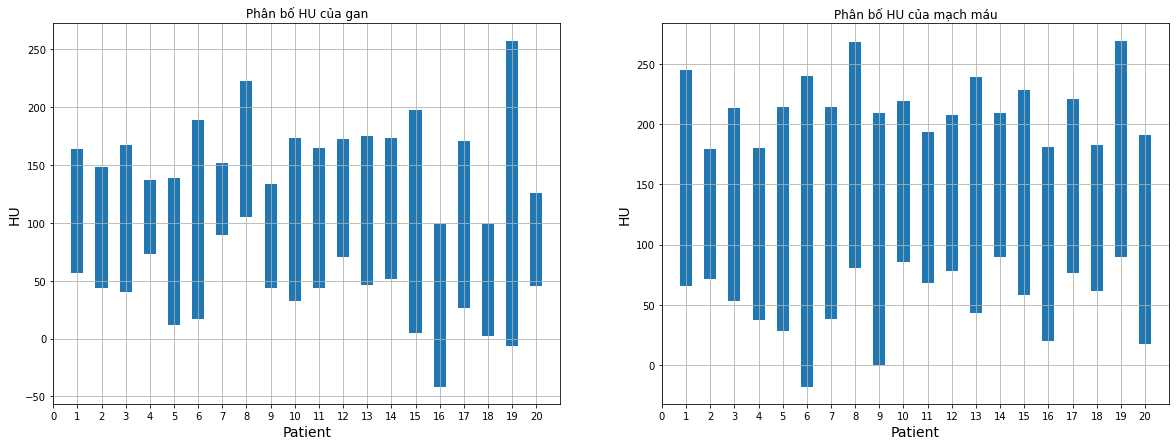
\includegraphics[width=13cm]{images/experiments/hu_dist.png}
		\caption{Phân bố giá trị HU từng bệnh nhân.}
		\label{hu_dist}
	\end{center}
	\begin{center}
		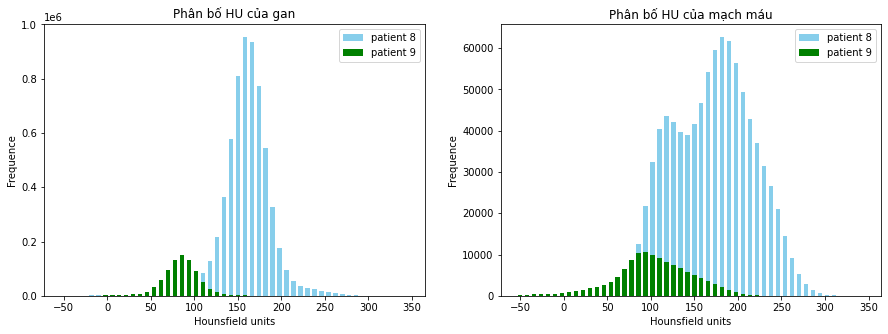
\includegraphics[width=13cm]{images/experiments/compare_2patient.png}
		\caption{So sánh phân bố HU của 2 bệnh nhân số 8 và số 9.}
		\label{hu_compare}
	\end{center}
\end{figure}
\vspace{-0.25cm}
Do đó, chúng tôi tiến hành chia tập dữ liệu thành 3 tập dữ liệu bao gồm: tập huấn luyện, tập kiểm thử, tập kiểm tra dựa trên phân phối giá trị trung bình HU của từng bệnh nhân.

\begin{table}[H]
    \centering
    \begin{tabular}{|c|l|l|l|l|c|}
    \hline
    \multicolumn{1}{|c|}{\multirow{2}{*}{\textbf{STT}}} & \multicolumn{1}{c|}{\multirow{2}{*}{\textbf{Tập}}} & \multicolumn{3}{c|}{\textbf{Phân phối giá trị trung bình HU}}       & \multirow{2}{*}{\textbf{Tổng}} \\ \cline{3-5}
    \multicolumn{1}{|c|}{}                     & \multicolumn{1}{c|}{}                     & \textless{}125 & {[}125 , 150{]}        & \textgreater 150 &                       \\ \hline
    0 & Huấn luyện   & 5, 16, 9, 18, 20  & 2, 3, 7, 12, 13, 14, 15 & 8, 10    & 14                    \\ \hline
    1 & Kiểm thử     & 4             & 17                     & 19          & 3                     \\ \hline
    2 & Kiểm tra     & 6             & 11                     & 1           & 3                     \\ \hline
    
    \end{tabular}
    \caption{Bảng phân chia các bệnh nhân thành các tập dữ liệu cho mạch máu.}
    \label{tab:training-set-vessel}
    \begin{tabular}{|c|l|l|l|l|c|}
    \hline
    \multicolumn{1}{|c|}{\multirow{2}{*}{\textbf{STT}}} & \multicolumn{1}{c|}{\multirow{2}{*}{\textbf{Tập}}} & \multicolumn{3}{c|}{\textbf{Phân phối giá trị trung bình HU}}       & \multirow{2}{*}{\textbf{Tổng}} \\ \cline{3-5}
    \multicolumn{1}{|c|}{}                     & \multicolumn{1}{c|}{}                     & \textless{}100 & {[}100 , 110{]}        & \textgreater 110 &                       \\ \hline
    0                                          & Huấn luyện                                & 2, 5, 9, 16, 17  & 1, 3, 10, 11, 15 & 7, 8, 13, 14       & 14                    \\ \hline
    1                                          & Kiểm thử                                  & 18             & 6                     & 12               & 3                     \\ \hline
    2                                          & Kiểm tra                                  & 20              & 4                     & 19              & 3                     \\ \hline
    \end{tabular}
    \caption{Bảng phân chia các bệnh nhân thành các tập dữ liệu cho gan.}
\end{table}

\subsection{Các phương pháp xử lý dữ liệu} \label{data-process}
Trong phần này, nhóm trình bày các công việc đã thực hiện để tiền xử lý dữ liệu bao gồm: lấy mẫu dữ liệu, chuẩn hóa dữ liệu, chia dữ liệu thành các khối nhỏ, tăng cường dữ liệu, trích xuất thành phần gan.
\subsubsection{Lấy mẫu dữ liệu}
Trong quá trình khảo sát các tập dữ liệu (cụ thể 3DIRCAD), chúng tôi nhận thấy khoảng cách thực giữa các điểm ảnh trong tập dữ liệu theo các chiều có sự chênh lệch lớn (Bảng \ref{voxelsize}). Điều này gây ảnh hưởng đến quá trình huấn luyện của mô hình bởi dữ liệu không đồng nhất. Do đó để chuẩn hóa dữ liệu, chúng tôi tiến hành lấy mẫu lại ảnh bằng cách đưa khoảng cách thực ban đầu về chung một giá trị đối với tất cả các ảnh. Về phương pháp thu phóng ảnh, chúng tôi sử dụng hàm nội suy bậc ba spline (do thư viện scipy cung cấp).

\begin{table}[H]
    \centering
    \begin{tabular}{|c|c|c|c|}
    \hline
    \textbf{STT} & \textbf{Giới tính} & \textbf{Kích thước voxel (mm)} & \textbf{Kích thước ảnh (pixels)} \\ \hline
    1   & Nữ  & 0.57 - 0.57 - 1.6  & 512 - 512 - 129 \\ \hline
    2   & Nữ  & 0.78 - 0.78 - 1.6  & 512 - 512 - 172 \\ \hline
    3   & Nam & 0.62 - 0.62 - 1.25 & 512 - 512 - 200 \\ \hline
    ... &     &                    &                 \\ \hline
    20  & Nữ  & 0.81 - 0.81 - 2.0  & 512 - 512 - 225 \\ \hline
    \end{tabular}
    \caption{Thông tin ảnh của tập dữ liệu 3DIRCAD (chi tiết có thể xem tại \cite{3dircad})}
    \label{voxelsize}
\end{table}

Việc lấy mẫu lại làm thay đổi đáng kể kích thước tập dữ liệu ban đầu (h - w - d). Một số chiều dữ liệu bị kéo dãn ra, một số chiều bị thu hẹp lại.

\begin{table}[H]
    \centering
    \begin{tabular}{|c|c|c|c|}
    \hline
    \multirow{2}{*}{\textbf{STT}} & \multirow{2}{*}{\textbf{Giới tính}} & \multicolumn{2}{c|}{\textbf{Kích thước ảnh sau khi nội suy (pixels)}}  \\ \cline{3-4}
     &  & \textbf{(1.0 - 1.0 - 1.0) mm} & \textbf{(0.5 - 0.5 - 0.5) mm} \\ \hline
    1   & Nữ  & 292 - 292 - 206  & 584 - 584 - 413 \\ \hline
    2   & Nữ  & 398 - 398 - 275 & 798 - 798 - 550 \\ \hline
    3   & Nam & 316 - 316 - 250 & 634 - 634 - 500 \\ \hline
    ... &     &                 &                 \\ \hline
    20  & Nữ  & 414 - 414 - 450 & 828 - 828 - 900 \\ \hline
    \end{tabular}
    \caption{Kết quả sau khi nội suy dữ liệu}
\end{table}

\subsubsection{Lấy ngưỡng giá trị Hounsfield Unit(HU)}
Để làm tăng độ tương phản giữa gan (mạch máu) và các bộ phận khác trong ảnh CT, một phương pháp được áp dụng phổ biến là chọn ngưỡng giá trị cho ảnh. Câu hỏi đặt ra lúc này là làm thế nào để chọn ngưỡng HU cho hợp lý? Chúng ta sẽ phân tích phân bố giá trị HU để chọn những giá trị ngưỡng phù hợp. Dưới đây là biểu đồ thể hiện phân phối giá trị HU của gan trên toàn bộ tập dữ liệu 3DIRCADB-01.

\begin{figure}[H]
    \centering
    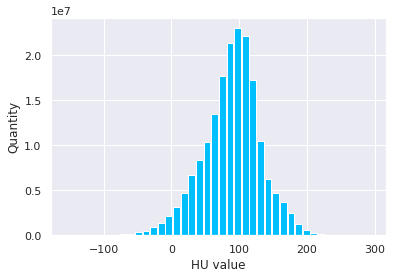
\includegraphics[width=10cm]{images/experiments/hu_dist_liver.png}
    \caption{Biểu đồ Hounsfield Units của tất cả các voxel chứa gan trên tập 3dircadb-01.}
\end{figure}
\vspace{-0.5cm}
Dựa vào biểu đồ trên, ta thấy giá trị HU của gan sẽ phân bố chủ yếu trên đoạn [-100, 250], do đó, ta sẽ chuẩn hóa dữ liệu bằng cách đưa các voxel có giá trị HU nhỏ hơn -100 về -100 và những voxel có giá trị lớn hơn 250 về 250. Nhờ vào đó ảnh trở lên tương phản hơn, đem lại thông tin rõ ràng hơn giữa các bộ phận. So sánh hình ảnh trước và sau khi thực hiện lấy ngưỡng giá trị HU:
\vspace{-0.5cm}
\begin{figure}[H]
    \centering
    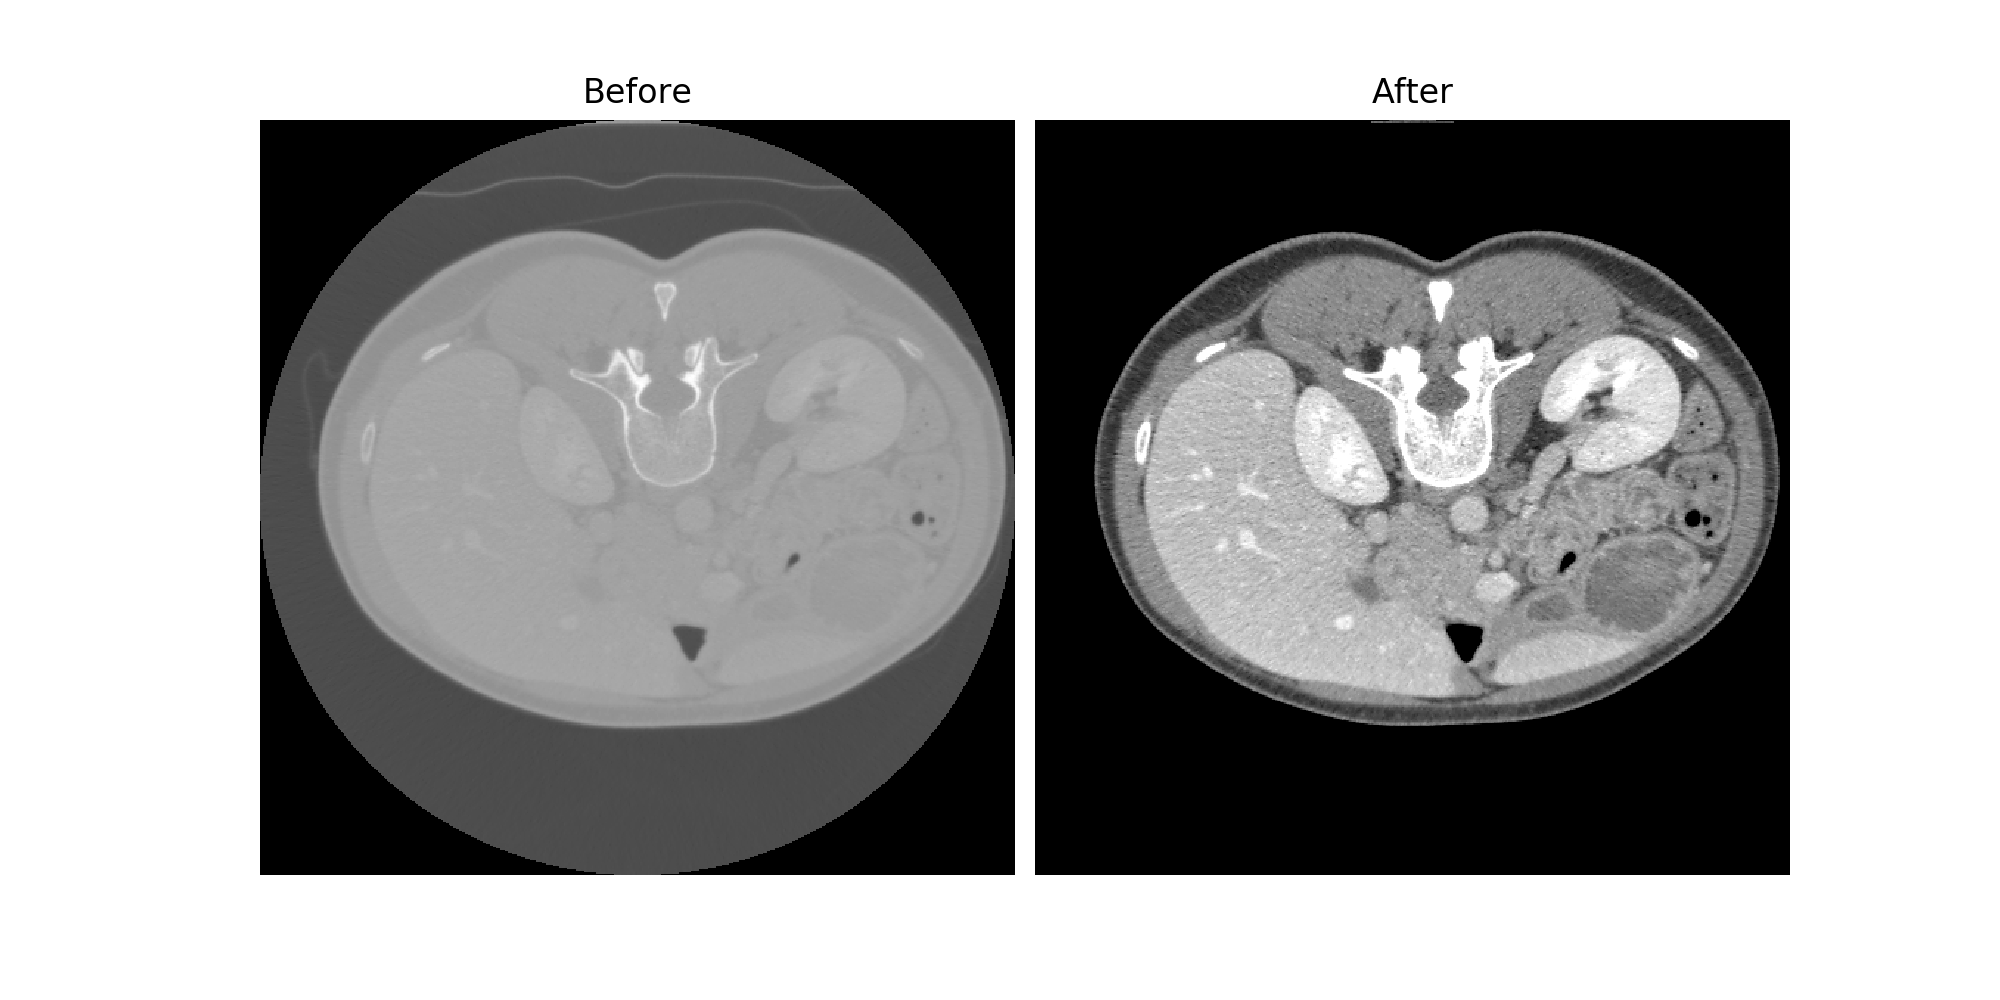
\includegraphics[width=10cm]{images/experience/HU-before-after.png}
    \caption{Kết quả trước và sau khi lấy ngưỡng giá trị HU.}
\end{figure}

\subsubsection{Chuẩn hóa dữ liệu}
Để tăng hiệu suất học tập của mô hình, sự phân bố giá trị của ảnh đầu vào góp phần quan trọng trong quá trình đạo hàm. Điều này khiến cho việc huấn luyện mô hình có khả thi hay không. Do đó, trước khi đưa vào huấn luyện, toàn bộ dữ liệu được chuẩn hóa dựa trên phương pháp biến đổi tuyến tính về đoạn [0, 1] theo công thức sau: \par
\vspace{-0.8cm}
\begin{align}
x' = \frac{(x-x_{min})}{(x_{max}-x_{min})}
\end{align}
Với x là ảnh ban đầu, x’ là ảnh sau khi chuẩn hóa, $x_{min}$, $x_{max}$ lần lượt là giá trị nhỏ nhất và lớn nhất trong ảnh.\par
\vspace{-0.5cm}

\subsubsection{Tăng cường dữ liệu}
Trong lĩnh vực ảnh y khoa, muốn gắn nhãn dữ liệu phải cần đến cấp độ chuyên gia, do đó không có nhiều dữ liệu để đào tạo mô hình. Việc huấn luyện mô hình với ít dữ liệu khó tạo ra kết quả tốt trong việc dự đoán. Kỹ thuật tăng cường dữ liệu (Data Augmentation) đã ra đời để giải quyết vấn đề này.\par
Các kĩ thuật tăng cường dữ liệu thường được sử dụng như:
\begin{itemize}[topsep=0pt]
    \item \textbf{Xoay}: xoay ảnh ban đầu theo một góc xác dịnh để thu được hình ảnh mới. Đối với ảnh CT, có thể xoay ảnh theo cả ba chiều.
    \item \textbf{Lật}: có thể lật ảnh theo chiều dọc hoặc chiều ngang.
    \item \textbf{Cắt ngẫu nhiên}: cắt ngẫu nhiên một phần của bức ảnh, lưu ý rằng ảnh sau khi cắt phải giữ lại phần mà ta quan tâm.
    \item \textbf{Biến dạng đàn hồi} (elastic transformation): dịch chuyển tọa độ các pixel của hình ảnh ban đầu tới vị trí mới để thu được hình ảnh bị biến dạng.
\end{itemize}
\begin{figure}[H]
    \centering
    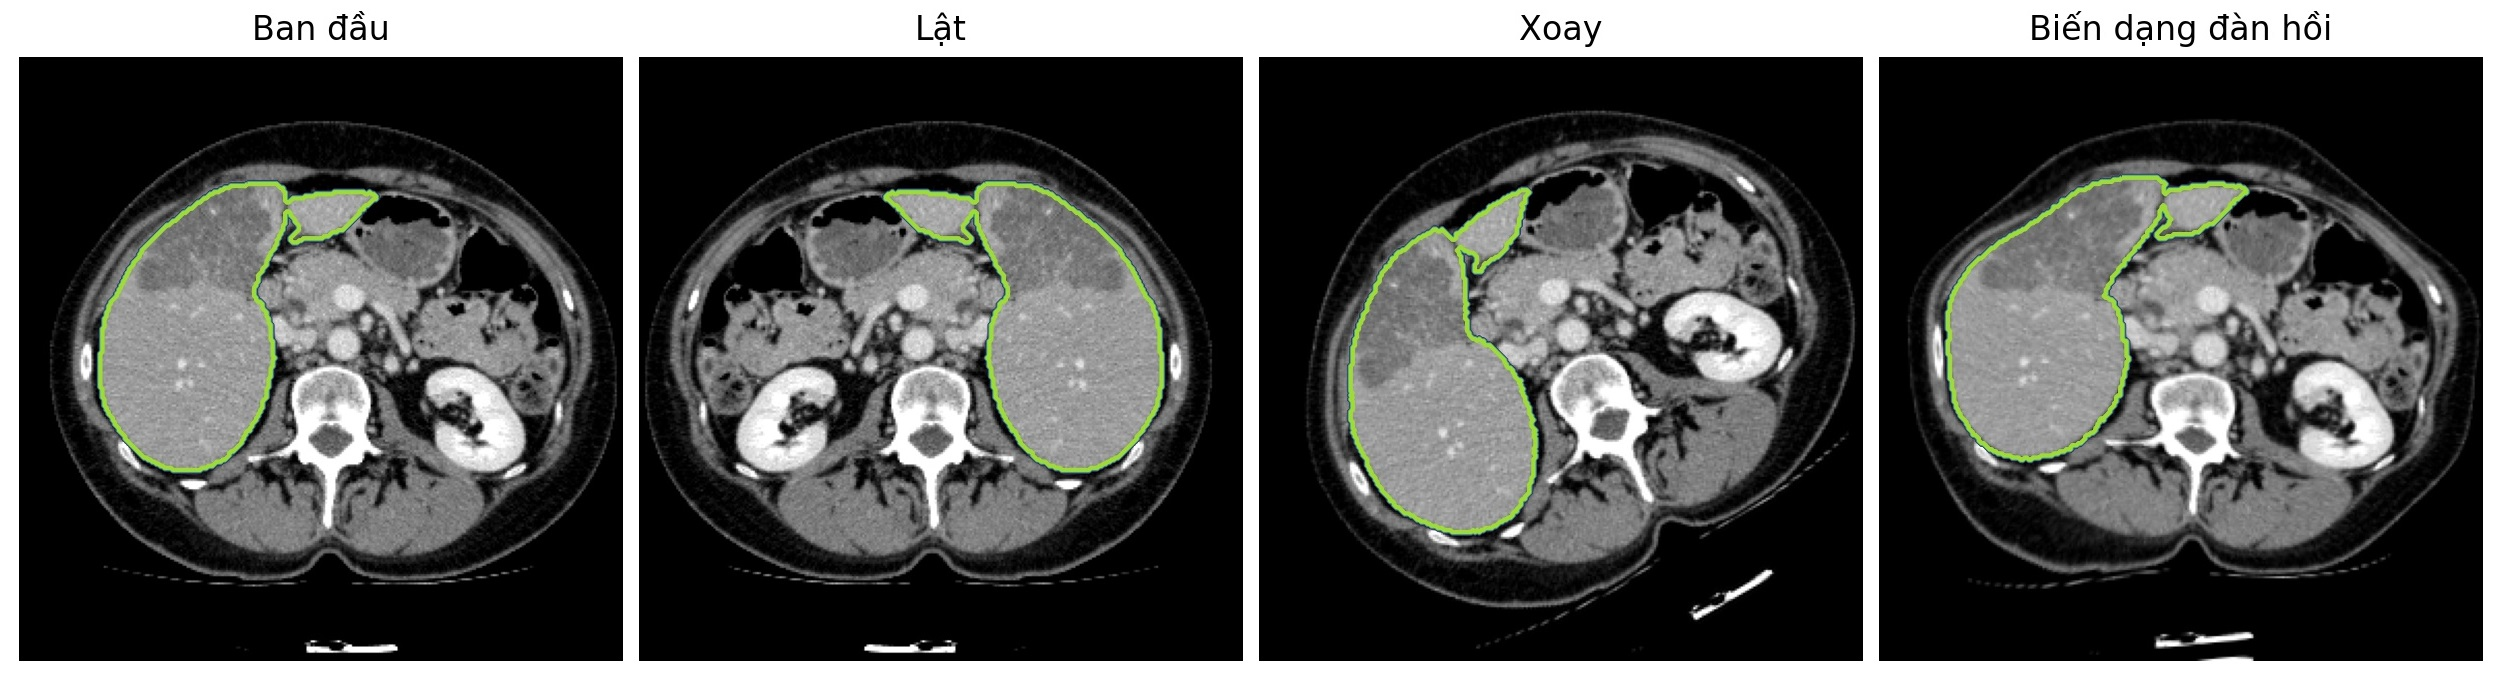
\includegraphics[width=14cm]{images/experience/aug.jpg}
    \caption{Ảnh trước và sau khi tăng cường dữ liệu}
\end{figure}
Thực tế khi chụp ảnh CT, bệnh nhân dược yêu cầu nằm ở một hướng cố định, kết quả là ảnh chụp cũng sẽ theo hướng cố định đó, việc lật và xoay ảnh sẽ không mang lại nhiều ý nghĩa trong thực tế. Tuy nhiên, việc có nhiều dữ liệu giúp mô hình học tập một cách tổng quát từ đó đem lại kết quả phân đoạn tốt hơn. Các phương pháp trên sẽ được nhóm sử dụng để tăng cường dữ liệu cho mô hình. \par

\subsubsection{Chia nhỏ dữ liệu}
Trong bài toán phân đoạn gan (mạch máu), dữ liệu ở dạng volume (mảng ba chiều) với kích thước lớn nhỏ khác nhau trong khi việc huấn luyện mô hình đòi hỏi dữ liệu đầu vào có cùng kích thước. Có nhiều cách để đưa dữ liệu về cùng kích thước như thêm đệm vào các volume kích thước nhỏ để đưa chúng về cùng kích thước với volume lớn nhất, thay đổi kích thước (resize) volume thành kích thước nhỏ hơn hoặc chia các volume thành nhiều sub-volume có kích thước giống nhau. Cách thứ nhất không khả thi vì giới hạn phần cứng, không thể huấn luyện mô hình với dữ liệu có kích thước lớn như vậy. Việc thay đổi kích thước volume như cách hai không bảo toàn khoảng cách không gian của các điểm dữ liệu, điều này làm mất đi ý nghĩa của việc nội suy để đưa các khoảng cách giữa ba chiều của các ảnh về cùng một giá trị như ở trên. Do đó, nhóm đã lựa chọn cách thứ ba là chia nhỏ volume ban đầu thành nhiều sub-volume có kích thước giống nhau.\par
Có nhiều cách để chia một volume thành nhiều sub-volume như chọn ngẫu nhiên, chia tuần tự,... Giả xử volume V ban đầu có kích thước D x H x W với D, H, W lần lượt là chiều sâu, chiều dài và chiều rộng của volume, sub-volume $S_{i}$ có kích thước là T x T x T.\par
\begin{itemize}
    \item \textbf{Chọn ngẫu nhiên}: chọn ngẫu nhiên một điểm nằm trong volume V có tọa độ $(x, y, z)$ làm điểm bắt đầu sau đó chọn sub-volume $S_{i} = V[x+T, y+T, z+T]$. Lặp lại quá trình này cho đến khi đủ số lượng sub-volume cần tạo. Phương pháp này có ưu điểm là kiểm soát được số lượng sub-volume được tạo ra nhưng cũng có nhược điểm là có thể một số vùng dữ liệu trong volume V bị bỏ sót. Điều này có thể được khắc phục bằng cách tăng số lượng mẫu cần lấy, khi đó xác suất để một vùng trong ảnh bị bỏ sót sẽ thấp xuống.
    \item \textbf{Chia tuần tự}: sử dụng một cửa sổ có kích thước bằng với kích thước sub-volume để trượt từ đầu cho đến cuối volume giống như cách lớp tích chập trích xuất đặc trưng. Volume V được chia nhỏ thành nhiều sub-volume $S_{i}$, các sub-volume này có thể chồng lấp lên nhau hoặc không. Đệm đã được thêm vào volume V để số lượng sub-volume tạo ra là số nguyên.
\end{itemize}
\begin{figure}[H]
    \centering
    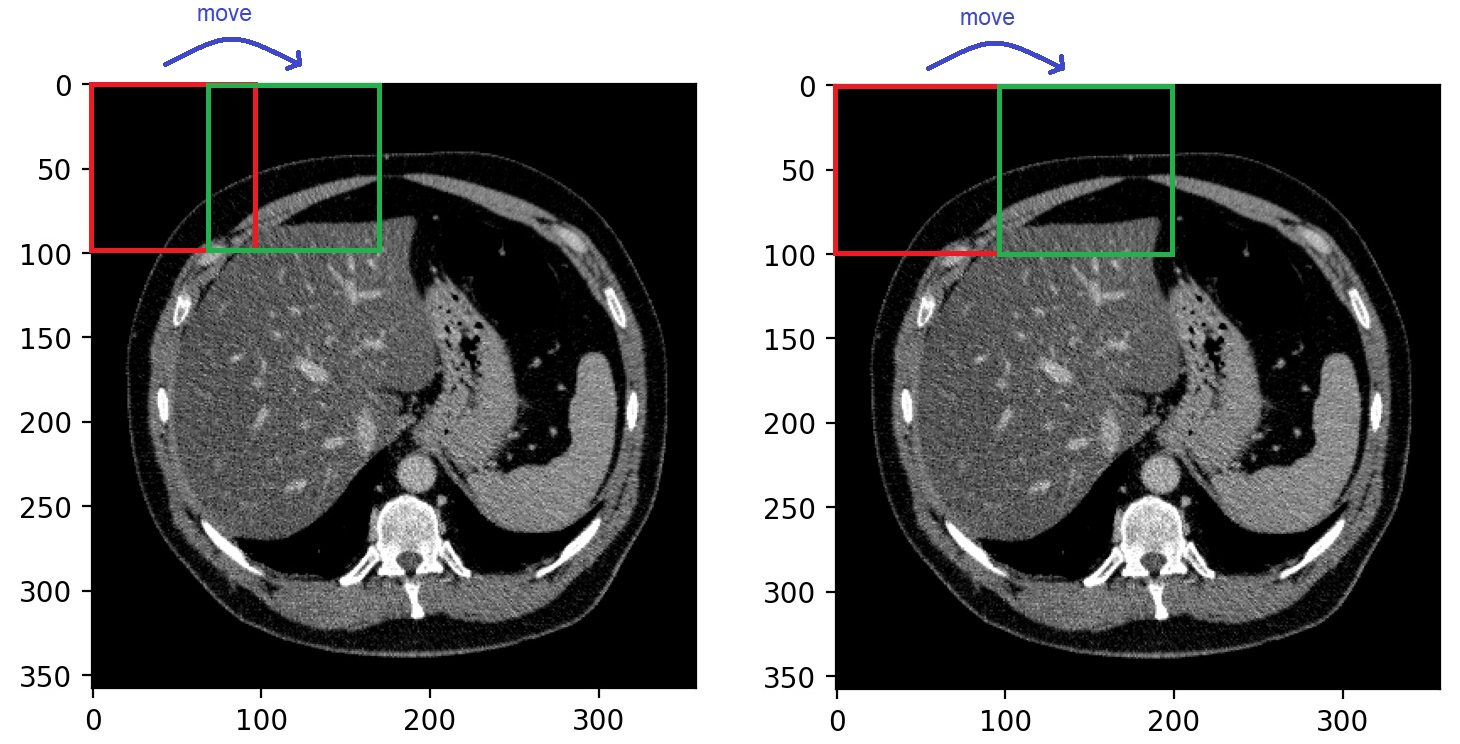
\includegraphics[width=12cm]{images/dataset/sub-volume-2d.jpg}
    \caption{Minh hoạ việc chia dữ liệu tuần tự}
    \label{2d_subvolume}
\end{figure} \par
Hình \ref{2d_subvolume} minh họa việc chia dữ liệu tuần tự trên một lát cắt (2D). Hình vuông màu đỏ là vị trí ban đầu của cửa sổ trượt, hình vuông màu xanh là vị trí tiếp theo. Ở hình bên trái, các sub-volume có chồng lấp lên nhau (phần giao nhau giữa hai hình vuông đỏ và xanh). Ở hình bên phải, các sub-volume nằm liên tiếp và không chồng lấp nhau. \par
Bước nhảy của cửa sổ trượt (stride) ảnh hưởng đến số lượng sub-volume được tạo ra. Nếu bước nhảy nhỏ hơn kích thước T, các sub-volume có chồng lấp lên nhau một phần, kết quả là tạo ra nhiều sub-volume hơn khi chia không chồng lấp. Nếu bước nhảy bằng T, các sub-volume sẽ nằm liên tiếp và không chồng lấp nhau. Nếu bước nhảy lớn hơn T, nhiều vùng dữ liệu sẽ bị bỏ sót, cách này sẽ không dược nhóm sử dụng trong các thí nghiệm sau này.

\subsubsection{Trích xuất thành phần gan}
Để tăng tính độ chính xác cho mô hình phân đoạn mạch máu, nhóm đã giới hạn lại phạm vi gắn nhãn cho mạch máu là chỉ quan tâm đến mạch máu nào thuộc vùng gan. Do đó đối với mô hình phân đoạn máu sẽ có sử dụng thêm một bước là trích xuất thành phần gan. Với điều này, chúng tôi đã giả định việc nhãn gan của ảnh CT là đã biết trước. Việc giả định nhãn gan có sẵn là khả thi trong thời điểm hiện tại, bởi hiên nay kết quả cao nhất trong lĩnh vực phân đoạn gan đã đạt trên 95\% d
độ chính xác. Do đó việc giả định này có thể chấp nhận được.

\begin{figure}[H]
    \centering
    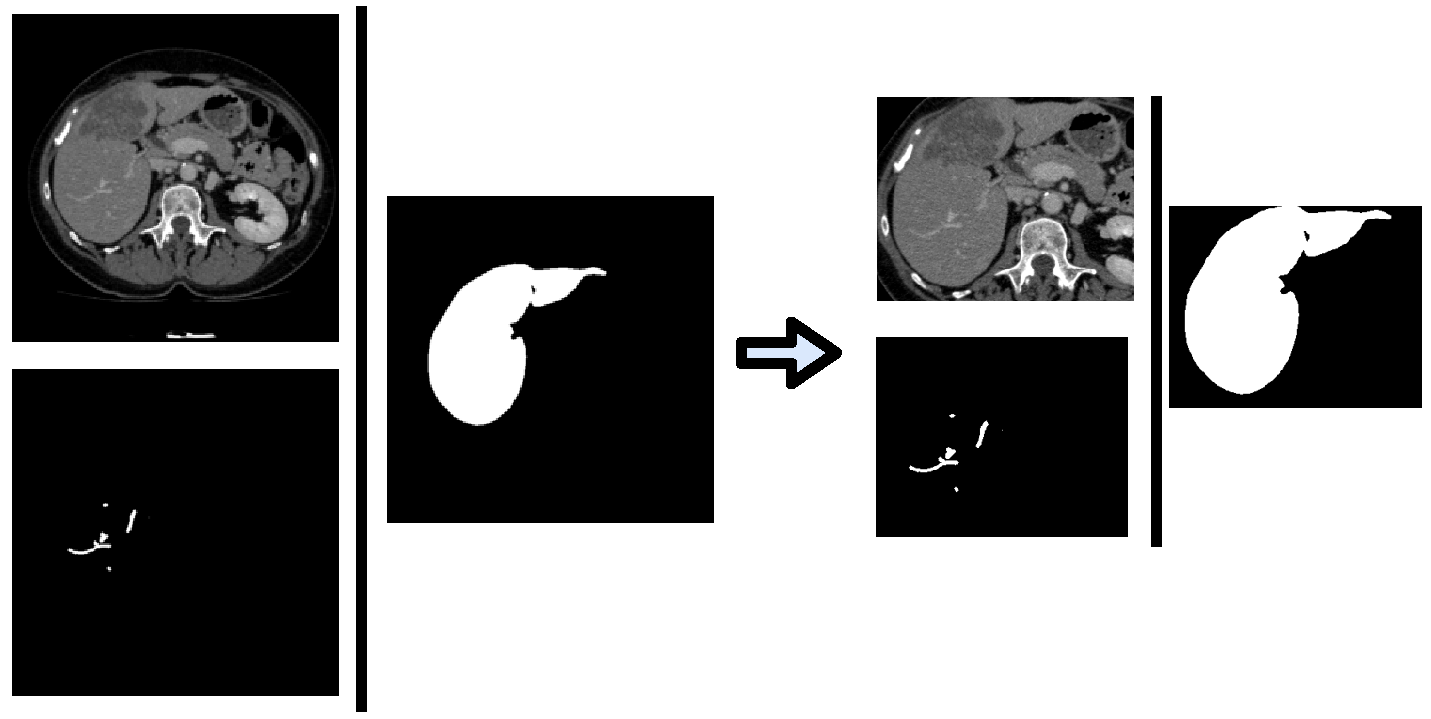
\includegraphics[width=12cm]{images/blood/extract_liver.pdf}
    \caption{Kết quả quá trình trích xuất thành phần gan.}
\end{figure}

\subsection{Trực quan hóa quy trình tiền xử lý}
\begin{enumerate}
    \item Lấy mẫu dữ liệu - đưa dữ liệu về kích thước chuẩn (1.0, 1.0, 1.0)mm đối với gan gà (0.5, 0.5, 0.5)mm đối với máu.
    \item Áp dụng ngưỡng dữ liệu [-100, 400].
    \item Chuẩn hóa HU về đoạn [0,1].
    \item Trích xuất thành phần gan.
    \item Chia tuần tự (hoặc ngẫu nhiên) thành các khối sub-volume nhỏ hơn.
\end{enumerate}
\begin{figure}[H]
    \centering
    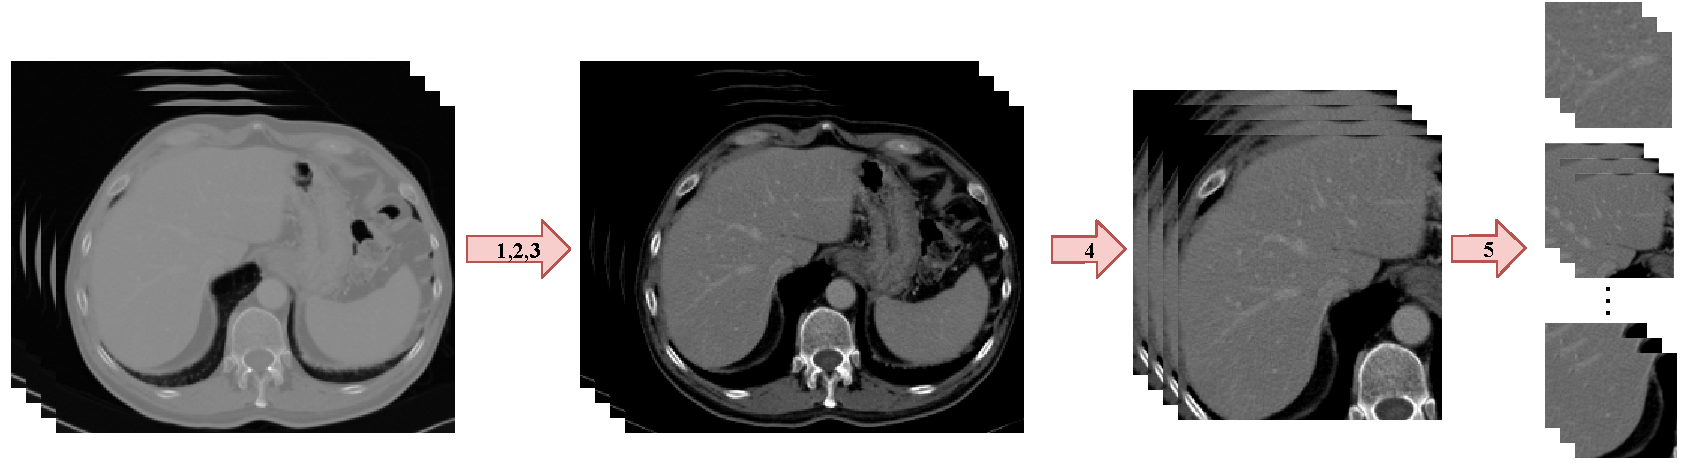
\includegraphics[width=14cm]{images/blood/preprocess_stage.pdf}
    \caption{Quy trình tiền xử lý.}
\end{figure}
    \chapter{PHƯƠNG PHÁP ĐỀ XUẤT}\label{chap:proposedmethod}
\textit{Chương này chúng tôi trình bày giải pháp mà chúng tôi đề xuất để giải quyết bài toán phân đoạn gan và mạch máu trên ảnh chụp cắt lớp vi tính. Bao gồm mô hình, hàm mục tiêu, quá trình huấn luyện. }

\section{Định nghĩa bài toán}
\textbf{Tổng quan bài toán:} Sau quá trình nghiên cứu và tìm hiểu các hệ thống phân đoạn hình ảnh y khoa , chúng tôi xác định được bài toán cần giải quyết bao gồm 3 nhiệm vụ chính: \textit{Huấn luyện mô hình gắn nhãn cho bộ phận gan và mạch máu, phát triển công cụ làm nhãn được cung cấp bởi GVLab đồng thời tích hợp mô hình phân đoạn tự động vào hệ thống}.
\vspace{-0.25cm}
\begin{itemize}
    \item[] \textbf{Dữ liệu đầu vào}
    \item Bộ ảnh CT 3 chiều của 1 bệnh nhân bất kỳ.
    \item Nhãn phân đoạn cơ quan tương ứng của bộ ảnh CT đó.
    
    \item[] \textbf{Dữ liệu đầu ra}
    \item Kết quả phân đoạn gan và mạch máu từ khối ảnh CT ban đầu.
\end{itemize}
\vspace{-0.25cm}
Sau khi xác định thông tin đầu vào và kết quả đầu ra của bài toán, chúng tôi đề xuất phương án thiết kế hệ thống với những tham khảo từ các công trình liên quan được trình bày trong phần tiếp theo.

\section{Hướng tiếp cận đề xuất}
Mô hình Unet2D \cite{Unet} đã đạt được nhiều kết quả khả quan trong lĩnh vực phân đoạn tế bào. Tuy nhiên, do có sự khác nhau về tính chất của 2 tập dữ liệu: bài báo Unet tập dữ liệu chỉ bao gồm những hình ảnh 2 chiều về tế bào trong khi đó tập dữ liệu về gan (máu) lại chứa thêm thông tin của chiều thứ 3 (là tập hợp các lớp cắt liên tiếp nhau trên cơ thể). Do đó việc quan tâm đến các thông tin không gian trong 3 chiều của các đối tượng có thể đem lại nhiều kết quả khả quan cho bài toán này. Bên cạnh đó, đã có nhiều công trình sử dụng Unet3D \cite{unet3d} làm mô hình chính để thực hiện các cải tiến và đạt những mục tiêu nhất định. Bên cạnh đó, nhờ vào những nghiên cứu trước trong lĩnh vực phân tích ảnh y khoa (\cite{Deepsupervision}, \cite{LV_LIVER}, \cite{LV_VESEL}), một mô hình đã đạt được độ chính xác đáng được nhắc tới là mô hình Unet3D sử dụng phương pháp giám sát sâu để huấn luyện \cite{Deepsupervision}. Mô hình này đã đạt được độ chính xác 95\% trong quá trình phân đoạn gan được \cite{LV_LIVER} triển khai. Do đó đây sẽ là mô hình cơ sở để nhóm phân tích phát triển các mô hình mới cho bài toán phân đoạn này. 

Kiến trúc U2net3D* được nhóm đề xuất được dựa trên ý tưởng của mô hình $\mathrm{U}^2$net (được giới thiệu ở phần \ref{u2net_arch}) cùng với mô hình Unet3D sử dụng giám sát sâu (Deep supervision). Đầu tiên để đánh giá mức độ hoạt động của 2 mô hình liên quan nhóm đã dựng lại các thí nghiệm áp dụng cho gan và mạch máu đối với 2 mô hình này (chi tiết ở chương \ref{chapter:experience}). 

Đối với mô hình $\mathrm{U}^2$net, đây là mô hình phân đoạn cho bài toán phát hiện đối tượng nổi bật trong ảnh với kích thước đầu vào ở dạng 2 chiều. Tuy nhiên, đối với việc xử lý 2 chiều trên ảnh CT không đạt hiệu quả cao bởi việc mất thông tin không gian ở chiều thứ 3 (có thể thấy ở thí nghiệm \ref{exp:2dvs3d}) hiện tại mục tiêu hướng tới của chúng tôi là sử dụng được chiều thứ 3 của ảnh CT, do đó nhóm đã tiến hành chuyển đổi dựa trên mô hình $\mathrm{U}^2$net sử dụng cho ảnh 3 chiều. Tuy nhiên bởi do tính chất của kiến trúc mạng quá lớn, việc chuyển giao qua mô hình 3D không thể thực thi. Số lượng tham số huấn luyện tăng từ 20 triệu tham số lên đến 100 triệu tham số cùng với việc số lượng bản đồ đặc trưng 3D trong quá trình tính toán tăng đáng kể. Do đó mô hình 3D theo kiến trúc $\mathrm{U}^2$net được bài báo đề xuất không thể huấn luyện tại thời điểm này vì không đủ phần cứng. Vì vậy, nhóm sẽ kế thừa ý tưởng kiến trúc khối Residual U-Block để phát triển. Khối Residual U-Block (RSU) sẽ có kiến trúc như hình \ref{img:Block}.a .

\begin{figure}[H]
    \subfloat[Residual U-Block -- RSU-3(In, M, Out)]{
    	\begin{minipage}[c][1.5\width]{0.5\textwidth}
    	   \centering
    	   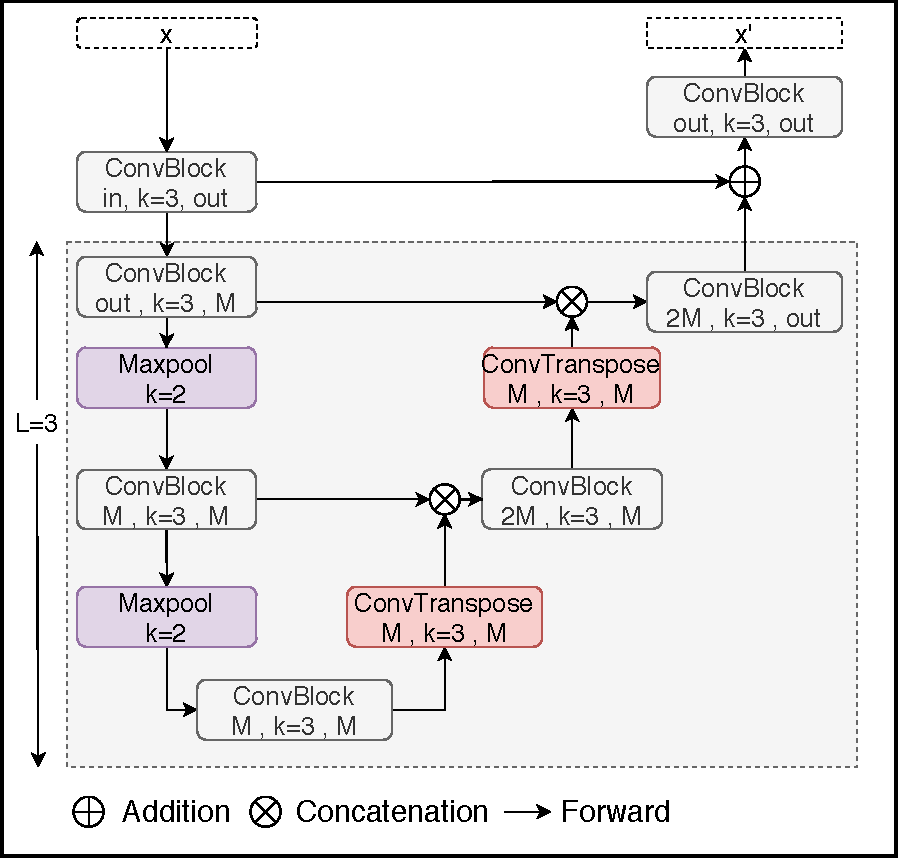
\includegraphics[width=1.35\textwidth]{images/blood/RSU_L3.pdf}
    	\end{minipage}}
	\hfill 	
    \subfloat[ConvBlock(In, M, Out)]{
    	\begin{minipage}[c][1.15\width]{0.65\textwidth}
    	   \centering
    	   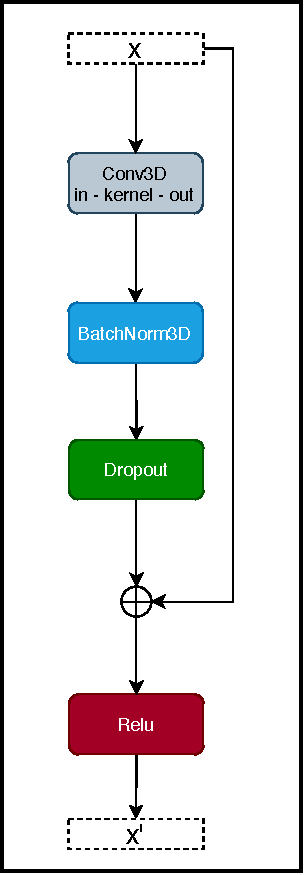
\includegraphics[width=0.4\textwidth]{images/blood/convblock.pdf}
    	\end{minipage}}
\caption{Kiến trúc các khối trong mô hình mạng}
\label{img:Block}
\end{figure}
\begin{itemize}
    \item Mỗi khối ConvBlock sẽ bao gồm các phép: Tích chập, Batchnorm, Dropout và hàm kích hoạt Relu. Bên cạnh đó khối có sử dụng phép kết nối tắt (residual) giúp hạn chế được tình trạng tiêu biến đạo hàm (vanishing gradient).
    \item Khối RSU sẽ bao gồm các siêu tham số: In, M, Out. Trong đó In là số kênh đầu vào của input, Out là số kênh đầu ra của các đặc trưng, M là số lượng các bản đồ đặc trưng được trích xuất trong các lớp trung gian. 
    \item[] Để lựa chọn các siêu tham số này một cách hợp lý, nhóm sẽ tiến hành các thí nghiệm trên các tham số khác nhau để kiểm chứng mô hình. 
\end{itemize}

\section{Kiến trúc mô hình phân đoạn đề xuất}\label{proposed-model}
Đầu tiên kế thừa sự thành công của mô hình CNN3D \cite{LV_LIVER} Nhóm đã chọn kiếm trúc này để làm mô hình cơ sở với ý tưởng tích hợp các khối RSU đại diện cho một kiến trúc Unet thu nhỏ vào mô hình CNN3D. Kiến trúc mô hình tổng quát dựa trên CNN3D như sau:
\begin{figure}[H]
    \centering
    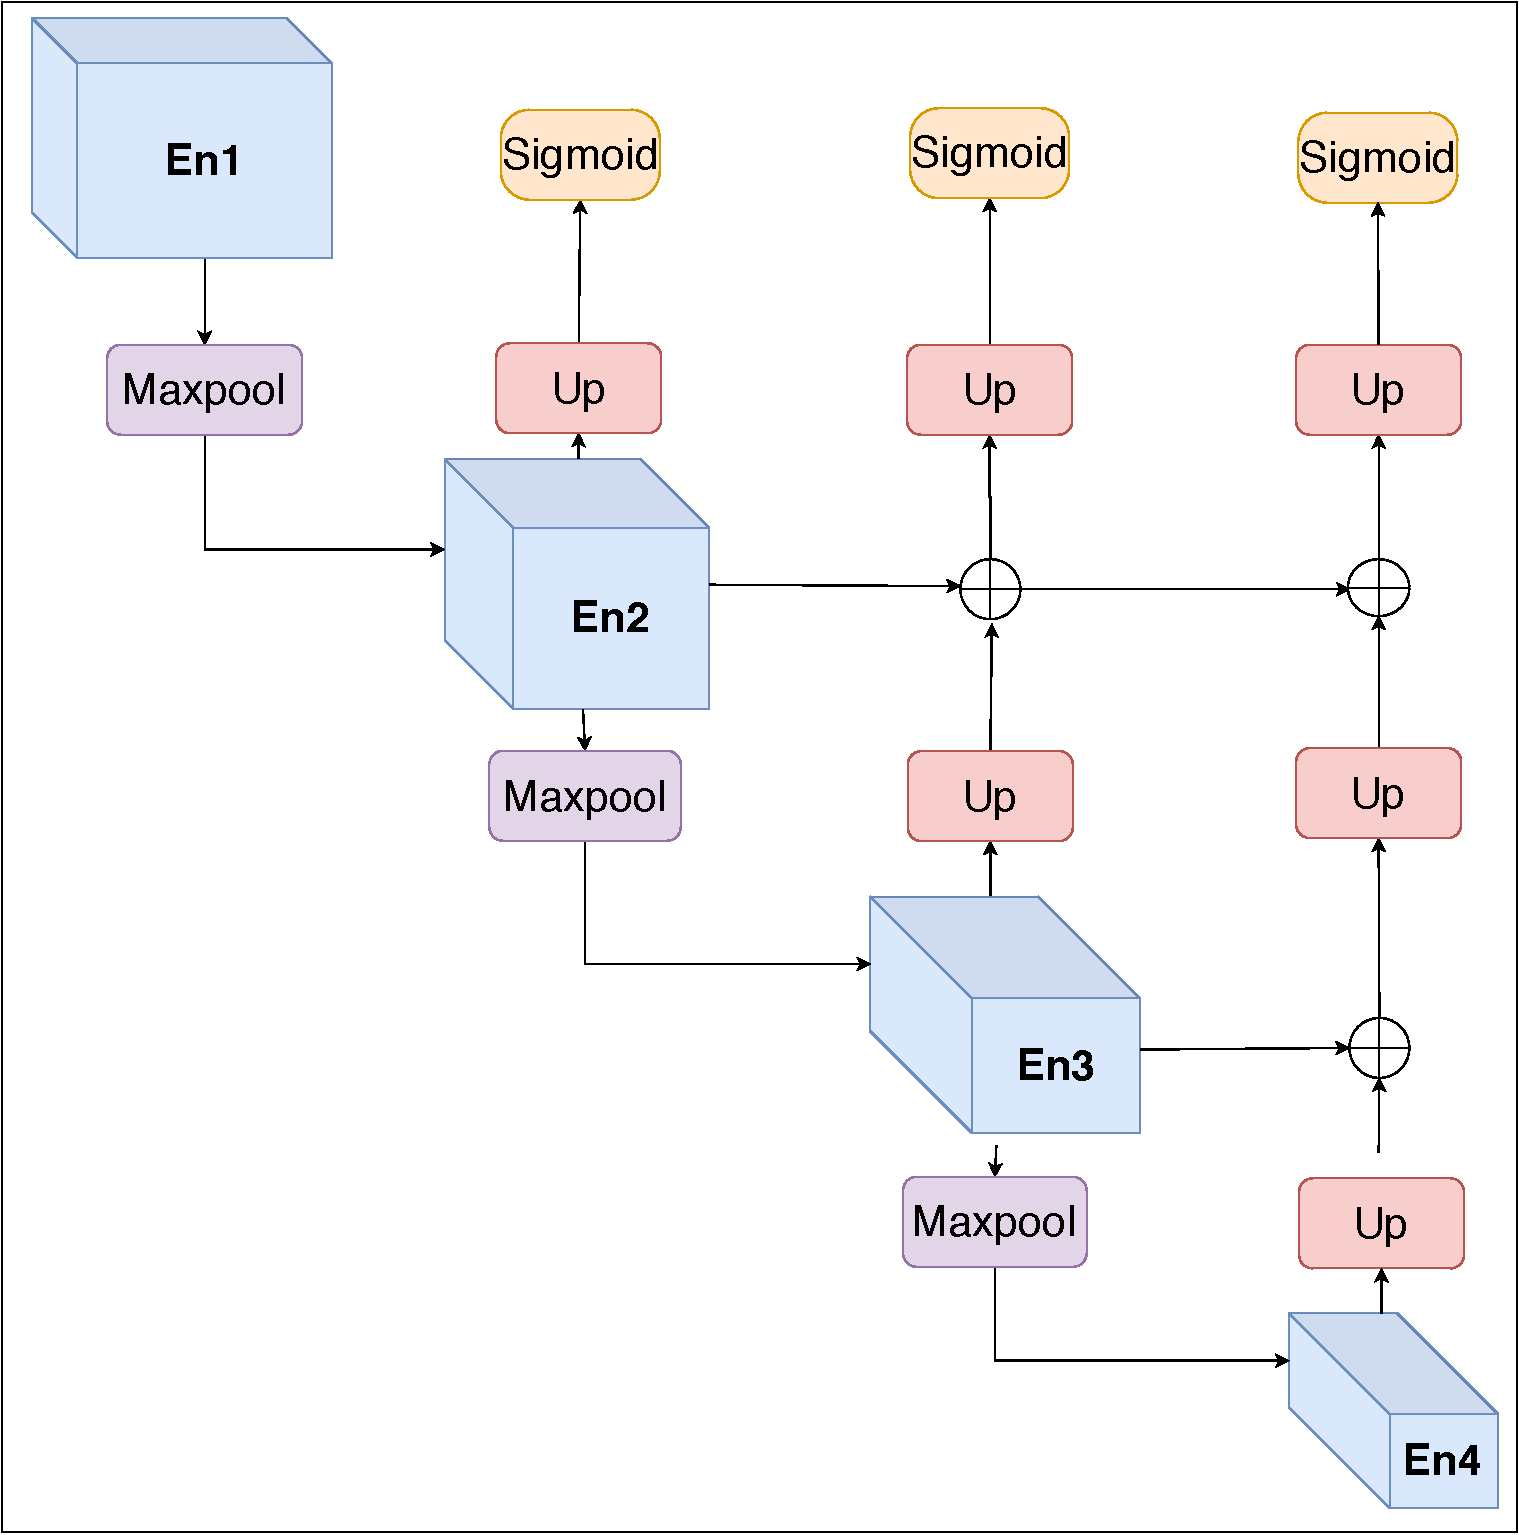
\includegraphics[scale=0.6]{images/blood/u2net3d-abstract.pdf}
    \caption{Kiến trúc mô hình tổng quát.}
    \label{fig:u2net3d-abstract}
\end{figure}

\newpage
\subsubsection{Khác biệt giữa kiến trúc mô hình đề xuất và mô hình CNN3D\cite{LV_LIVER}}
\begin{enumerate}
    \item Thay vì việc sử dụng các khối tích chập liên tiếp nhau trong quá trình mã hóa thông tin đầu vào, nhóm xin đề xuất việc thay những khối tích chập này thành những mô hình Unet thu nhỏ có tên là RSU.
    \item Ngoài ra, các phép kết nối tắt giữa các đặc trưng trích xuất trong bộ mã hóa sẽ được kết nối với đặc trưng từ bộ giải mã (có thể so sánh sự khác biệt này dựa trên hình \ref{fig:CNN3D} và Hình \ref{fig:u2net3d-abstract}). Nhờ vào các kết nối tắt này, các đặc trưng được sinh ra trong quá trình giải mã sẽ được kết hợp với thông tin ngữ cảnh trước đó giúp tăng độ chính xác của quá trình giải mã. Ngoài ra còn phần nào giúp được việc hạn chế quá trình tiêu biến đạo hàm.
\end{enumerate}
\vspace{-1cm}
\subsubsection{Bộ mã hóa}
\begin{enumerate}
    \item[] Bộ mã hóa của mô hình U2net3D* bao gồm 4 khối. 
    \item Khối En1 là khối tích chập thông thường bao gồm 2 khối ConvBlock (hình \ref{img:Block}.b)(mỗi khối bao gồm các phép tích chập, batchnorm, dropout, relu) liên tiếp nhau tại tầng thứ nhất. 
    \item Tại tầng thứ 2 trở đi sẽ là các khối RSU với số tầng của mỗi khối giảm 1 sau qua tầng tiếp theo. Khối RSU đầu tiên có số tầng là 3.  
    \item Thông qua các thí nghiệm chọn các siêu tham số cho mạng, chúng tôi nhận thấy việc sử dụng số lượng bản đồ đặc trưng đầu ra tăng gấp đôi sau mỗi tầng đạt được kết quả tốt nhất thay vì đặt tất cả các khối cùng một số lượng các đặc trưng trích xuất qua mỗi lớp.
\end{enumerate} 
\vspace{-1cm}
\subsubsection{Bộ giải mã}
\begin{enumerate}
    \item Các đặc trưng được sinh ra trong quá trình trích xuất thông tin của các khối RSU sẽ được giải mã tương ứng trên từng nhánh. Khi giải mã tới các tầng tương ứng, bộ giải mã sẽ sử dụng phép kết nối tắt dựa trên thông tin trước đó của từng tầng. Điều này giúp cho mô hình học tốt hơn bởi giá trị đầu vào sẽ được phân bố học dựa trên các luồng, các đặc trưng sinh ra tại mỗi tầng sẽ được giám sát song song với kết quả đầu ra cuối cùng.
    \item Các đặc trưng ở lớp cuối cùng của bộ giải mã sẽ đi qua lớp tích chập có bộ lọc 1x1x1 để thu giảm số kênh, sau đó qua lớp kích hoạt Sigmoid sẽ thu được giá trị xác xuất dự đoán của từng voxel.
\end{enumerate}

\begin{figure}[H]
    \centering
    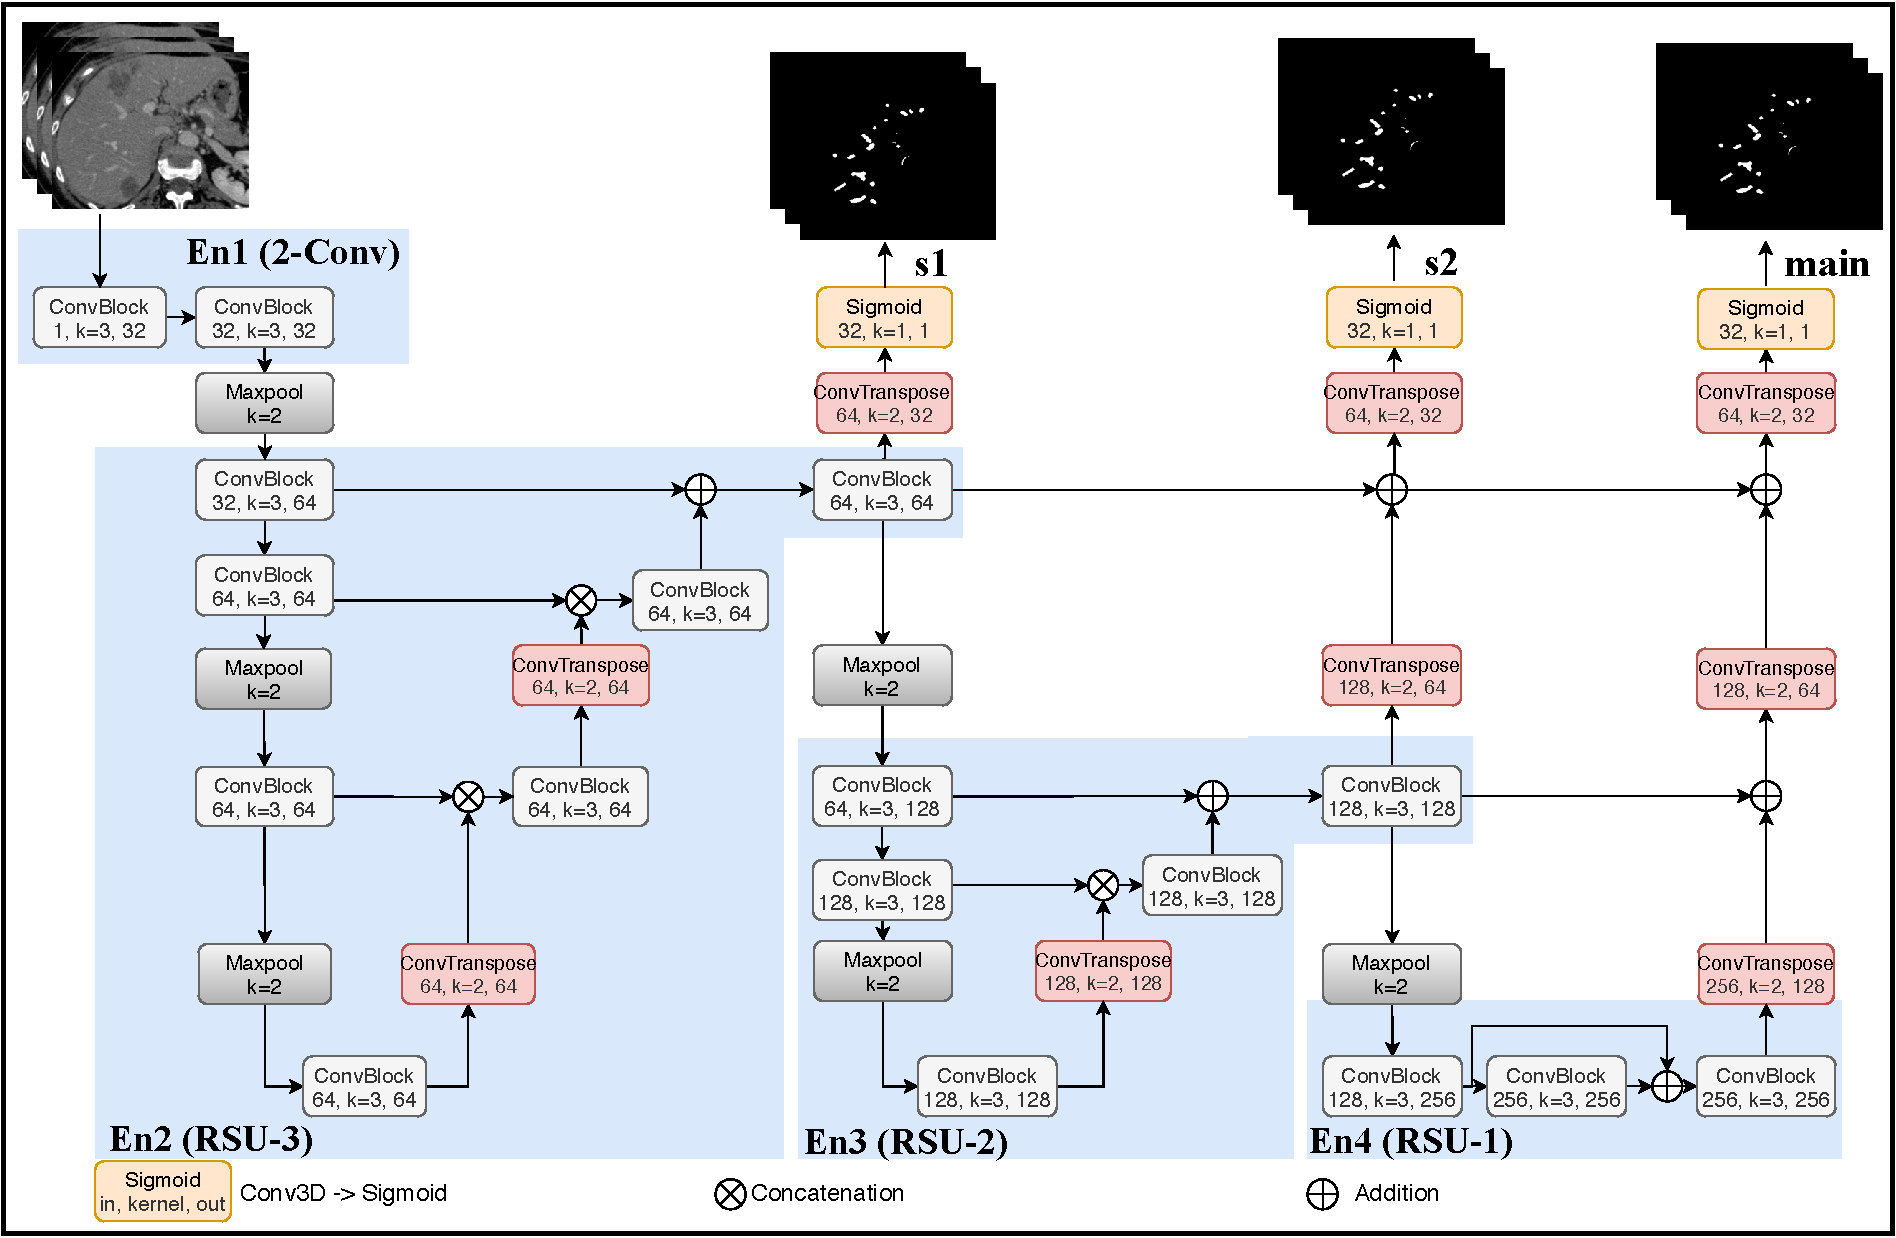
\includegraphics[angle=90,scale=0.6]{images/blood/u2net3d_arch.pdf}
    \caption{Kiến trúc mô hình chi tiết U2net3D*.}
    \label{fig:u2net3d-arch}
\end{figure}

\section{Hàm mục tiêu}
Trong bài toán học có giám sát (supervised learning), hàm mục tiêu (Objective Function) đóng vai trò quan trọng trong việc đưa ra giá trị phạt cho mô hình dự đoán sai bao nhiêu so với thực tế. Dựa vào đó, mô hình học cách cải thiện để đem lại kết quả tốt hơn sau mỗi lần học. Một số hàm mục tiêu được nhóm sử dụng để huấn luyện mô hình sẽ được trình bày bên đưới. Tất cả các hàm đều dùng cho bài toán phân đoạn nhị phân (2 lớp).

\subsubsection*{Binary Cross-Entropy Loss}
Hàm Binary Cross-Entropy (BCE) được dùng để đo lường tương quan giữa 2 phân phối xác suất dự đoán (q) và phân phối xác xuất thực tế (p).

\begin{align}
    \mathrm{L(q,p)} = -\sum_{i=1}^{C} \mathrm{p}_i \mathrm{log(q}_i)
\end{align}

Với $\sum_{i=1}^{C}\mathrm{p}_i = \sum_{i=1}^{C}\mathrm{q}_i = 1$ và C=2 đại diện cho 2 lớp cần dự đoán. Khi phân phối p và phân phối q càng tương quan thì giá trị của hàm BCE càng nhỏ, ngược lại khi hai phân phối này không tương quan giá trị hàm này sẽ càng lớn. Do đó, chúng ta đi tối ưu hàm Binary Cross Entropy cũng đồng nghĩa đi huấn luyện mô hình dự đoán phân phối q gần với phân phối p nhất. Đối với bài toán có 2 lớp giá trị nhãn $p_i$ sẽ nhận 2 giá trị 0 và 1. Do đó công thức trên có thể viết lại thành: 

\begin{align}
    \mathrm{L(q, p}) = -\log(\mathrm{q}) \\
    \nonumber
    \mathrm{q} = \begin{cases} 
              \mathrm{q} & \text{if } p = 1 \\
              1-\mathrm{q} & \text{otherwise}
          \end{cases}
\end{align}

Dựa vào đồ thị \ref{Focal-effective-weight} với gamma=0 (đây chính là đồ thị cho BCELoss) có thể thấy khi $\mathrm{q}$ tiến dần đến 1 thì hàm BCE tiến dần đến 0 - trường hợp mô hình tốt nhất tức là phân phối giữa p và q trùng nhau. Còn khi $\mathrm{q}$ tiến dần đến 0 thì hàm BCE tiến dần đến $\infty$ - mô hình tệ nhất. 

\subsubsection*{Focal Loss}
Đối với các bài toán bị mất cân bằng dữ liệu quan trọng, hàm BCE sẽ không hoạt động 1 cách hiệu quả. Ví dụ trong trường hợp bài toán phân đoạn ảnh, một bức ảnh có 100 pixel trong đó có 5 pixel là của nhãn A và số còn lại là của nhãn B. Một mô hình sẽ tiến hành phân loại và sử dụng hàm BCE để đánh giá cho từng pixel. Giá trị hàm loss sẽ là trung bình của tất cả giá trị BCE của 100 pixel này.  Như vậy, nếu mô hình chúng ta phân loại tốt lớp B nhưng không thể phân loại được lớp A điều này sẽ khiến cho hàm loss đem lại giá trị loss trung bình 100 pixel rất thấp vì 95 pixel đã được dự đoán đúng và chỉ 5 pixel thuộc lớp A dự đoán sai. Dễ nhận thấy đây là trường hợp tệ nhất mà chúng ta muốn tránh.

Do đó, với đề xuất của bộ phận nghiên cứu AI Facebook, họ đã đề xuất một sự cải tiến hàm Cross Entropy có trọng số được gọi là Focal Loss  (FL) được giới thiệu trong bài báo 'Focal Loss for Dense Object Detection' \cite{focal}. Với mục tiêu là cố gắng giảm sự đóng góp của các pixel vào trong giá trị loss tổng thay vì 100 pixel có mức độ ưu tiên như nhau ở ví dụ trên.

Với $\alpha$, $\gamma$ là các siêu tham số, giá trị $\alpha$ nằm giữa 0 và 1 để cân bằng tỉ lệ mẫu dương và mẫu âm. Giá trị $\alpha$ càng lớn thì độ đóng góp giá trị loss các mẫu dương sẽ càng cao hơn. Giá trị $\gamma > 0$ , có tác dụng làm giảm độ quan trọng của mẫu các mẫu phân loại đúng khi đóng góp vào giá trị của loss tổng. Như vậy $\gamma$ càng cao, hàm mục tiêu sẽ càng chú ý vào các mẫu bị phân loại sai, và giảm giá trị phạt cho các mẫu phân loại đúng. 

Công thức của hàm Focal Loss như sau:

\begin{align}
    \mathrm{FL(q, p)} &= -\alpha(1-\mathrm{q})^\gamma \log(\mathrm{q})\\
    \nonumber
    \alpha = \begin{cases} 
                    \alpha & \text{if } p = 1 \\
                    1-\alpha & \text{otherwise}
                \end{cases}
    &\quad and \quad
    \mathrm{q} = \begin{cases} 
              \mathrm{q} & \text{if } p = 1 \\
              1-\mathrm{q} & \text{otherwise}
          \end{cases}
\end{align}

Dựa vào đồ thị \ref{Focal-effective-weight} ta có thể thấy $\gamma$ càng lớn, kết hợp với các giá trị dự đoán đúng càng nhiều thì giá trị loss càng giảm mạnh. Như vậy nó sẽ góp phần đóng vai trò ít hơn trong hàm loss tổng. Chính nhờ vào điều này ta sẽ cân bằng được số lượng mẫu như ví dụ trên trong việc góp phần vào giá trị hàm mục tiêu.
\begin{figure}[H]
    \centering
    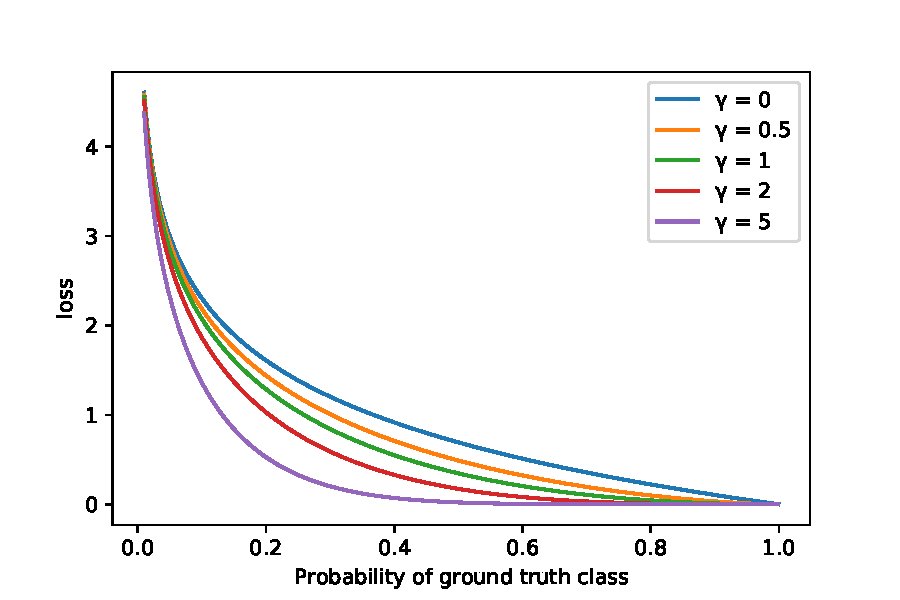
\includegraphics[width=10cm]{images/blood/focal.pdf}
    \caption{Sự ảnh hưởng của trọng số $\gamma$ đối với hàm focal loss $\mathrm{FL(q)=-(1-q)^\gamma \mathrm{log}(q)}$ }
    \label{Focal-effective-weight}
\end{figure}

\subsubsection*{Dice Loss}
Đây là hàm mất mát thường được sử dụng cho bài toán mất cân bằng giữa các lớp. Bằng cách lấy 1 trừ đi giá trị Dice, ta được công thức của Dice Loss:
\begin{align}
    L = 1 - 2\frac{\sum_{1}^{N}p_i*q_i}{\sum_{1}^{N}p_i + \sum_{1}^{N}q_i}
\end{align}
Trong đó, N là tổng số điểm ảnh. $p_i$ và $q_i$ lần lượt là giá trị nhãn và giá trị dự đoán của điểm ảnh thứ i, với $p_i \in \left \{ 0, 1 \right \}$ và $q_i \in \left [ 0, 1 \right ]$.

\section{Phương pháp huấn luyện}
\textbf{Phương pháp huấn luyện giám sát sâu}: Một số phần giải mã (decoder) thích hợp đã được thêm vào mạng để huấn luyện theo \textbf{phương pháp giám sát sâu}. Theo phương pháp này, hàm mất mát sẽ được tính từ hàm mất mát của tất cả các phần giải mã:
\begin{align}
    Loss = \mu_{1}Loss_{s1} + \mu_{2}Loss_{s2} + \mu_{3}Loss_{main}
    \label{LossU2net3D}
\end{align}

Mô hình sẽ có ba đầu ra, do đó hàm lỗi tổng sẽ có 3 thành phần tương ứng với từng đầu ra. Độ quan trọng của các đầu ra được xác định dựa trên giá trị của các siêu tham số $\mu_{1}$, $\mu_{2}$ và $\mu_{3}$. Hàm mất mát toàn phần lúc này là tổng hợp của hàm mất mát chính và các hàm mất mát phụ. Quá trình cập nhật tham số sẽ được chia sẻ giữa các luồng thay vì chỉ trên luồng chính. Cơ chế này giúp mô hình hội tụ nhanh hơn và có độ chính xác cao hơn. 

Hàm loss được sử dụng trong các thí nghiệm bao gồm 2 hàm BCELoss và Focal Loss (sử dụng độc lập với nhau) được sử dụng trong các thí nghiệm ở chương \ref{chapter:experience}.

Các siêu tham số sẽ được đặt tương ứng $\mu_1=1, \mu_2=2,  \mu_3=4$ với mục đích tăng dần độ quan trong trong quá trình giám sát việc trích xuất các đặc trưng theo từng tầng. Giá trị đầu ra của tầng cuối cùng sẽ chiếm phần quan trọng nhất và chính là kết quả cuối cùng của quá trình phân đoạn.

	\chapter{THÍ NGHIỆM VÀ ĐÁNH GIÁ}\label{chapter:experience}
\vspace{-0.5cm}
\noindent\textit{Trong phần này nhóm sẽ trình bày các thí nghiệm về việc huấn luyện mô hình dựa trên những thay đổi về kiến trúc mô hình, các siêu tham số mô hình, hàm lỗi, dữ liệu huấn luyện ... để đánh giá các ưu nhược điểm đang gặp phải hiện tại đối với việc phân đoạn gan và mạch máu.}\par

\section{Tổng quan}
\subsection{Môi trường thí nghiệm}
\subsubsection{Thông tin phần cứng}
Huấn luyện mạng học sâu với lượng lớn dữ liệu đòi hỏi sức mạnh tính toán cao để công tác huấn luyện diễn ra nhanh chóng và hiệu quả. Để đáp ứng yêu cầu đó, nhóm đã sử dụng hệ thống máy tính hiệu năng cao (HPCC) do GVLab cung cấp. Ngoài ra, nhóm cũng sử dụng Google Colab pro để có thể huấn luyện song song nhiều mô hình.\par

\begin{table}[H]
\centering
\begin{tabular}{@{}ccl@{}}
\toprule
\textbf{STT}       & \textbf{Nguồn cung cấp}       & \multicolumn{1}{c}{\textbf{Cấu hình}}                                             \\ \midrule
\multirow{2}{*}{1} & \multirow{2}{*}{GVLab} & \begin{tabular}[c]{@{}l@{}}GPU: NVIDIA Tesla V100 32GB\\ RAM: 126 GB\end{tabular} \\ \cmidrule(l){3-3} 
                   &                        & \begin{tabular}[c]{@{}l@{}}GPU: NVIDIA Tesla P100 16GB\\ RAM: 126 GB\end{tabular} \\ \midrule
2                  & Google Colab Pro       & \begin{tabular}[c]{@{}l@{}}GPU: NVIDIA Tesla P100 16GB\\ RAM: 12 GB\end{tabular}  \\ \bottomrule
\end{tabular}
\caption{Thông tin phần cứng}
\label{tab:hardware}
\end{table}

\subsubsection*{Ngôn ngữ và framework}
\begin{itemize}[topsep=0pt]
    \item Ngôn ngữ: Python 3.6.9
    \item Framework: PyTorch 1.6.0+cu101
\end{itemize}

\subsection{Phương pháp đánh giá}
Đối với bài toán này, các độ đo được sử dụng để đánh giá mô hình là: Dice, Recall, VOE và VD. Thông tin chi tiết về các độ đo này đã được trình bày ở phần \ref{evaluation-methods}

\section{Thí nghiệm mô hình Unet}

%%%%%%%%%%%%%%%%%%%%%%%%% Mau %%%%%%%%%%%%%%%%%%%%%%%%%%%%%%%%%
\subsection{Thí nghiệm cho đối tượng mạch máu}
\subsubsection{Thí nghiệm về độ sâu của mô hình Unet3D}
Bởi vì sự khác nhau về kích thước giữa các đối tượng (mạch máu, gan) nên việc lựa chọn độ sâu của mô hình đóng phần quan trọng bởi đặc tính của các lớp tích chập và lớp gộp. Nếu mô hình đi càng sâu thì thông tin toàn cục sẽ được chú ý nhiều hơn là thông tin cục bộ, điều này có thể khiến cho mô hình tệ hơn như đã đề cập ở \ref{sec:Unet3D}. 

Nhóm tiến hành huấn luyện mạng Unet3D với các độ sâu khác nhau để tìm được độ sâu (số tầng) phù hợp với mô hình. Các thí nghiệm đều sử dụng hàm đánh giá mất mát: Focal loss với hệ số $\gamma=2$ và $\alpha=0.8$. Kết quả được tính dựa trên trung bình từng hệ số đánh giá cho từng bộ ảnh trong tập kiểm tra. Kết quả tốt nhất thu được trên từng thí nghiệm như sau:

\begin{table}[H]
\centering
\begin{tabular}{c|c|c|c|c}
\Xhline{3\arrayrulewidth}
\multirow{2}{*}{\textbf{Mô hình}} & \multirow{2}{*}{\textbf{Độ sâu}} & \multicolumn{2}{c|}{\textbf{Tập kiểm tra}} & \multirow{2}{*}{\textbf{Số lượng tham số}} \\ 
\cline{3-4} 
&       &\textbf{Dice}       & \textbf{Recall}    &                 \\ \hline
Unet3D  & 3 & 51.58               & 51.33              & 5.420.737       \\ \hline
Unet3D  & 4 & \textbf{55.33}      & 59.06              & 22.399.425      \\ \hline
Unet3D  & 5 & 36.04               & \textbf{65.13}     & 90.304.449      \\

\Xhline{3\arrayrulewidth}
\end{tabular}
\caption{Kết quả thí nghiệm về độ sâu mô hình Unet3D}
\end{table}

Có thể thấy mô hình Unet3D 4 tầng đạt được kết quả khả quan hơn so với độ sâu 3 và 5. Kết quả này có sự khác biệt với mô hình gan bởi vì gan có kích thước lớn hơn máu rất nhiều do đó gan cần mô hình có độ sâu sâu hơn để có được vùng receptive field (vùng mà nơ ron nhìn thấy) rộng hơn để phân biệt được đó có phải là bộ phân gan hay không. Từ thí nghiệm này, nhóm sẽ chọn mô hình Unet3D 4 tầng làm mô hình chính để thực hiện biến đổi cho các thí nghiệm sau.

\subsubsection{So sánh giữa mô hình Unet2D và mô hình Unet3D} \label{exp:2dvs3d}
Để đánh giá được độ hiệu quả của việc phân tích thông tin dưới dạng 3 chiều, nhóm đã tiến hành huấn luyện mạng Unet2D với các thông số giống mạng 3D như mục trên để tiến hành đánh giá. Kiến trúc mạng chỉ được thay đổi các lớp tích chập và lớp gộp từ 3D thành 2D. Và kết quả thí nghiệm như sau:

\begin{table}[H]
    \centering
    \begin{tabular}{c|c|c c| c}
    \Xhline{3\arrayrulewidth}
    \multirow{2}{*}{\textbf{Mô hình}} & \multirow{2}{*}{\textbf{Độ sâu}} & \multicolumn{2}{c|}{\textbf{Tập kiểm tra}} & \multirow{2}{*}{\textbf{Số lượng tham số}} \\ 
    \cline{3-4}
             & & \textbf{Dice} & \textbf{Recall} &  \\ \hline
    Unet2D   & 4 & 41.17 & \textbf{60.05} & 7.701.825 \\ \hline
    Unet3D   & 4 & \textbf{55.33}  & 59.06  & 22.399.425 \\ 
    
    \Xhline{3\arrayrulewidth}
    \end{tabular}
    \caption{Kết quả thí nghiệm mô hình Unet2D và Unet3D}
\end{table}
\vspace{-0.6cm}

Có thể thấy mô hình Unet3D 4 tầng cho ra kết quả tốt hơn Unet2D 4 tầng. Do đó việc sử dụng thông tin 3 chiều đã đem lại lợi thế nhất định, giúp mô hình 3 chiều có kết qủa phân đoạn cải thiện hơn so với mô hình 2 chiều. Việc đánh giá cũng được thực hiện giống nhau trên cùng tập dữ liệu và đều lấy trung bình từ kết quả từng bộ ảnh CT 3 chiều.

\subsubsection{Thí nghiệm chọn siêu tham số cho hàm mục tiêu}
Để chọn được các siêu tham số cho hàm FocalLoss một cách hợp lý. Nhóm đã thiết lập các thí nghiệm tương ứng như sau để chọn được hệ số $\gamma$ và $\alpha$ thích hợp nhất cho mô hình.

\begin{table}[H]
    \centering
    \begin{tabular}{c c c c c c}
    \Xhline{3\arrayrulewidth}
    \multirow{2}{*}{\textbf{Hàm lỗi}} & \multicolumn{2}{c}{\textbf{Siêu tham số}} & \multicolumn{2}{c}{\textbf{Tập kiểm thử}} \\ \cline{2-5}
     & \textbf{gamma} & \textbf{alpha} & \textbf{Dice} & \textbf{Recall} \\
    \hline
    BCE Loss   & \_  & \_  & 54.17 & 42.66 \\
    \hline
    Focal Loss & 1.0 & 0.6 & 52.59 & 45.19\\
    Focal Loss & 1.0 & 0.7 & 50.98 & 47.96\\
    Focal Loss & 1.0 & 0.8 & 53.98 & 48.11\\
    Focal Loss & 1.5 & 0.7 & 53.05 & 49.43\\
    Focal Loss & 1.5 & 0.8 & 53.23 & 50.18\\
    Focal Loss & 2.0 & 0.7 & 54.16 & 54.07\\
    Focal Loss & 2.0 & 0.8 & \textbf{55.33}  & 59.06\\
    Focal Loss & 3.0 & 0.8 & 50.12 & \textbf{59.10}\\
    \Xhline{3\arrayrulewidth}
    \end{tabular}
    \caption{Kết quả thí nghiệm các siêu tham số hàm mục tiêu.}
    \label{table:focal}
\end{table}
\vspace{-0.65cm}
Qua kết quả bảng \ref{table:focal} cho ta thấy được, khi $\alpha$ tăng thì độ truy hồi (Recall) cũng tăng bởi $\alpha$ càng lớn thì trọng số của mẫu dương (mạch máu) càng cao do đó độ dự đoán chính xác của mạch máu sẽ tăng đáng kể. Bên cạnh đó, khi tăng $\gamma$ có nghĩa là trong quá trình phạt kết quả huấn luyện, hàm mục tiêu sẽ chú tâm vào những mẫu bị phân loại sai hơn bằng cách làm giảm hệ số đóng góp của các mẫu được phân loại đúng vào hàm loss tổng. Nhờ đó quá trình phạt các mẫu sẽ trở nên cân bằng hơn giúp hạn chế việc mất cân bằng dữ liệu. Hiện tại hệ số $\gamma=2$ và $\alpha$=0.8 đã cho kết quả tốt nhất trong các thí nghiệm, do đó 2 siêu tham số này sẽ được dùng trong các thí nghiệm sau để tiên hành quá trình huấn luyện.
%%%%%%%%%%%%%%%%%%%%%%%%% Mau (end) %%%%%%%%%%%%%%%%%%%%%%%%%%%
\subsection{Thí nghiệm cho đối tượng gan}
\subsubsection{Thí nghiệm về tập dữ liệu} \label{liver-dataset-exp}
Dữ liệu huấn luyện là tri thức của mô hình để nó có thể đưa ra những dự đoán. Việc có nhiều dữ liệu giúp mô hình học tập và đưa ra dự đoán tổng quát hơn. Hiện nay, theo khảo sát của nhóm, có ba tập dữ liệu có nhãn về gan được công khai, đó là: Sliver07, Lits17 và 3Dircadb. Nhóm sẽ thí nghiệm và so sánh kết quả khi trộn các tập dữ liệu với nhau với kết quả trên từng tập riêng rẽ.

\subsubsection{Tiền xử lý dữ liệu}
Mỗi tập Sliver07, Lits17 và 3Dircadb được chia thành các tập huấn luyện, kiểm thử và kiểm tra dựa trên trung bình HU của gan (tham khảo phần \ref{data-preparation}). Tập \textbf{Mixed} được tạo thành bằng cách trộn tương ứng các tập huấn luyện, kiểm thử và kiểm tra của ba tập trên với nhau. Thông tin chi tiết về số lượng dữ liệu như bảng bên đưới:\par
\begin{table}[H]
\renewcommand{\arraystretch}{1.2}
\centering
\begin{tabular}{c|c|c|c} 
\Xhline{3\arrayrulewidth}
 \textbf{Tập dữ liệu} & \textbf{Huấn luyện} & \textbf{Kiểm thử} & \textbf{Kiểm tra} \\ 
 \hline
 Sliver07 & 14 & 3 & 3 \\ 
 \hline
 Lits17 & 101 & 15 & 15 \\ 
 \hline
 3Dircadb & 14 & 3 & 3 \\ 
 \hline
 Mixed & 129 & 21 & 21 \\ 
\Xhline{3\arrayrulewidth}
\end{tabular}
\caption{Số lượng volume huấn luyện, kiểm tra, kiểm thử trên các tập dữ liệu}
\end{table}
\raggedbottom
Các bước xử lý dữ liệu được thực hiện tuần tự như sau (xem chi tiết ở phần \ref{data-process}):
\begin{itemize}[noitemsep, topsep=0pt]
    \item \textbf{Lấy mẫu dữ liệu}: tiến hành nội suy toàn bộ các volume và nhãn tương ứng để đưa khoảng cách không gian giữa các điểm dữ liệu về kích thước \textbf{1mm}.
    \item \textbf{Chuẩn hóa}: tiến hành lấy ngưỡng giá trị HU, đưa ngưỡng giá trị của các volume về đoạn $[-100, 250]$ sau đó thực hiện phép biến đổi tuyến tính đưa dữ liệu về đoạn $[0, 1]$.
    \item \textbf{Sinh mẫu}: chia tuần tự mỗi volume trong tập huấn luyện và kiểm thử thành các sub-volume không chồng lấp nhau (bước nhảy của cửa sổ trượt bằng kích thước sub-volume).
    \item \textbf{Lọc mẫu}: loại bỏ những mẫu không chứa gan trên tập huấn luyện và kiểm thử.
\end{itemize}

\subsubsection{Huấn luyện mô hình}
Dữ liệu sau khi tiền xử lý sẽ được sử dụng để huấn luyện mô hình. Thông số huấn luyện mô hình cụ thể như sau:
\begin{itemize}
    \item Tập dữ liệu: Sliver07, Lits17, 3Dircadb, Mixed.
    \item Kích thước mẫu: 96 x 96 x 96.
    \item Mô hình: Unet3D 3 tầng.
    \item Hàm lỗi: Dice loss.
    \item Hệ số học: 1e-5.
    \item Kích thước Batch: 5.
    \item Điều kiện dừng: 10 epoch kết quả Dice kiểm thử không cải thiện.
\end{itemize}

\subsubsection{Đánh giá kết quả}
Kết quả kiểm tra là trung bình kết quả của tất cả các volume trong tập kiểm tra. Với mỗi bộ ảnh, quá trình thực hiện như sau:
\begin{itemize}[noitemsep, topsep=0pt]
    \item Tiến hành lấy mẫu bằng phương pháp nội suy volume và nhãn tương ứng để đưa khoảng cách giữa các điểm dữ liệu về 1mm.
    \item Chia volume thành các sub-volume.
    \item Dự đoán kết quả trên từng sub-volume.
    \item Gọp kết quả dự đoán trên các sub-volume lại thành volume dự đoán.
    \item Dựa vào volume dự đoán và nhãn để đánh giá kết quả phân đoạn.
\end{itemize}
\subsubsection{Kết quả thí nghiệm}

\begin{table}[H]
\renewcommand{\arraystretch}{1.2}
\centering
\begin{tabular}{c|c|c|c}
\Xhline{3\arrayrulewidth}
\multicolumn{2}{c|}{\textbf{Thí nghiệm}} & \multicolumn{2}{c}{\textbf{Độ đo}}       \\ \hline
\textbf{Huấn luyện  }               & \textbf{Kiểm tra}     & \textbf{Dice} (\%) & \textbf{Recall} (\%) \\ \hline
\multicolumn{2}{c|}{Sliver07}          & 84.68                         & 92.62                           \\ \hline
\multicolumn{2}{c|}{Lits17}            & 79.09                         & 84.88                           \\ \hline
\multicolumn{2}{c|}{3Dircadb}          & 60.62                         & 91.78                           \\ \hline
\multirow{4}{*}{Mixed} & Sliver07          & $\uparrow 87.18$                         & 86.52                           \\ \cline{2-4} 
                       & Lits17            & $\uparrow 81.93$                         & 90.63                           \\ \cline{2-4} 
                       & 3Dircadb          & $\uparrow 87.61$                         & 89.89                           \\ \cline{2-4} 
                       & Mixed             & 83.49                         & 89.93                           \\ 
\Xhline{3\arrayrulewidth}
\end{tabular}
\caption{Kết quả kiểm tra thí nghiệm về các tập dữ liệu}
\end{table}

Có thể thấy việc huấn luyện trên tập Mixed và kiểm tra trên các tập còn lại cho kết quả tốt hơn việc huấn luyện và kiểm tra trên từng tập riêng rẽ. Điều này cho thấy hiệu quả của việc có càng nhiều dữ liệu trong huấn luyện, mô hình học sâu càng tổng quát. Tập Mixed sẽ được nhóm sử dụng xuyên suốt trong các thí nghiệm phía sau.

\subsubsection{Thí nghiệm về kích thước đầu vào} \label{liver-input-size}
Để kiểm chứng ảnh hưởng của kích thước đầu vào đối với việc huấn luyện mô hình, nhóm đã thực hiện các thí nghiệm với các kích thước đầu vào mô hình khác nhau.
Thí nghiệm được thực hiện trên tập Mixed với các kích thước sub-volume là $64 \times 64 \times 64$, $96 \times 96 \times 96$, $128 \times 128 \times 128$ và $160 \times 160 \times 160$. Quá trình tiền xử lý dữ liệu, thông số huấn luyện mô hình, cách đánh giá kết quả tương tự như thí nghiệm về tập dữ liệu (\ref{liver-dataset-exp}) \par
Kết quả thí nghiệm thu được như bảng bên dưới:
\begin{table}[H]
\renewcommand{\arraystretch}{1.2}
\centering
\begin{tabular}{c|c|c}

\Xhline{3\arrayrulewidth}
\multirow{2}{*}{\textbf{Thí nghiệm}} & \multicolumn{2}{c}{\textbf{Độ đo}}        \\ \cline{2-3} 
                                     & \textbf{Dice} (\%) & \textbf{Recall} (\%) \\ \hline
$64 \times 64 \times 64$        & 71.69          & 88.66          \\ \hline
$96 \times 96 \times 96$        & \textbf{83.49} & \textbf{89.93} \\ \hline
$128 \times 128 \times 128$     & 80.12          & 85.81          \\ \hline
$160 \times 160 \times 160$     & 80.94          & 87.81          \\
\Xhline{3\arrayrulewidth}
\end{tabular}
\caption{Kết quả kiểm tra thí nghiệm kích thước đầu vào}
\end{table}
Khi tăng kích thước đầu vào từ 64 lên 96, kết quả kiểm tra tăng lên đáng kể, kết quả này giảm khi tiếp tục tăng kích thước lên 128, 160. Nhóm quyết định dừng lại ở kích thước 160 vì đây là kích thước tương đối lớn và hơn nữa kết quả tốt nhất là khi sub-volume có kích thước $96 \times 96 \times 96$. \par
Để tìm kích thước đầu vào tối ưu hơn, nhóm đã tiếp tục thí nghiệm với kích thước nhỏ hơn 96 và lớn hơn 64 là $80 \times 80 \times 80$ và một kích thước khác lớn hơn 96 và nhỏ hơn 128 là $112 \times 112 \times 112$. Kết quả thu được như sau:\par
\begin{table}[H]
\renewcommand{\arraystretch}{1.2}
\centering
\begin{tabular}{c|c|c}
\Xhline{3\arrayrulewidth}
\multirow{2}{*}{\textbf{Thí nghiệm}} & \multicolumn{2}{c}{\textbf{Độ đo}}        \\ \cline{2-3} 
                                     & \textbf{Dice} (\%) & \textbf{Recall} (\%) \\ \hline
$64 \times 64 \times 64$        & 71.69          & 88.66          \\ \hline
$80 \times 80 \times 80$        & 74.08          & 89.42          \\ \hline
$96 \times 96 \times 96$        & \textbf{83.49} & \textbf{89.93} \\ \hline
$112 \times 112 \times 112$        & 75.11          & 89.17          \\ \hline
$128 \times 128 \times 128$     & 80.12          & 85.81          \\ \hline
$160 \times 160 \times 160$     & 80.94          & 87.81          \\ 
\Xhline{3\arrayrulewidth}
\end{tabular}
\caption{Kết quả kiểm tra thí nghiệm kích thước đầu vào}
\end{table}
Hai thí nghiệm mới không đem lại kết quả tốt hơn. Kích thước tối ưu của sub-volume tìm được là $96 \times 96 \times 96$. Kích thước này sẽ được sử dụng cho các thí nghiệm phía sau.\par
Việc sử dụng kích thước đầu vào lớn nhưng không cải thiện kết quả có thể là do mô hình còn đơn giản, chưa có nhiều lớp tích chập, dẫn tới vùng nhìn thấy (receptive field) của lớp cuối cùng đạt tới giới hạn và không cải thiện nữa.\par

\subsubsection{Thí nghiệm về độ sâu mô hình}
Độ sâu mô hình có ảnh hưởng đến kết quả phân đoạn. Mô hình đủ sâu (phức tạp) sẽ khái quát hóa được dữ liệu và đem lại kết quả tốt hơn. Nhóm tiến hành thí nghiệm các độ sâu khác nhau của mô hình Unet3D. Thông tin thí nghiệm cụ thể như sau:
\begin{table}[H]
\renewcommand{\arraystretch}{1.2}
\centering
\begin{tabular}{c|c|c|c}
\Xhline{3\arrayrulewidth}
\textbf{STT} & \textbf{Số tầng} & \textbf{Số channels phần mã hóa (Encoder)} & \textbf{Số lượng tham số} \\ \hline
1     & 3       & $64 \to 128 \to 256$                   & 5.418.177   \\ \hline
2     & 4       & $64 \to 128 \to 256 \to 512$           & 22.393.793  \\ \hline
3     & 5       & $64 \to 128 \to 256 \to 512 \to 1024$  & 90.292.673  \\ 
\Xhline{3\arrayrulewidth}
\end{tabular}
\caption{Thông số thí nghiệm độ sâu mô hình}
\end{table}

Quá trình tiền xử lý dữ liệu, thông số huấn luyện mô hình, cách đánh giá kết quả tương tự như các thí nghiệm trước đó.

\begin{itemize}
    \item Tập dữ liệu: Mixed.
    \item Kích thước mẫu: 96 x 96 x 96.
    \item Mô hình: Unet3D-3 tầng, Unet3D-4 tầng, Unet3D-5 tầng.
    \item Hàm lỗi: Dice loss.
    \item Hệ số học: 1e-5.
    \item Kích thước Batch: 5.
    \item Điều kiện dừng: 10 epoch kết quả Dice kiểm thử không cải thiện.
\end{itemize}

Kết quả thí nghiệm như sau:
\begin{table}[H]
\renewcommand{\arraystretch}{1.2}
\centering
\begin{tabular}{c|c|c}
\Xhline{3\arrayrulewidth}
\multirow{2}{*}{\textbf{Thí nghiệm}} & \multicolumn{2}{c}{\textbf{Độ đo}}        \\ \cline{2-3} 
                                     & \textbf{Dice} (\%) & \textbf{Recall} (\%) \\ \hline
Unet3D-3 tầng       & 83.49          & 89.93          \\ \hline
Unet3D-4 tầng       & \textbf{88.17} & 90.49          \\ \hline
Unet3D-5 tầng       & 88.09 & \textbf{94.20}          \\ 
\Xhline{3\arrayrulewidth}
\end{tabular}
\caption{Kết quả kiểm tra thí nghiệm độ sâu mô hình}
\label{tab:deep-model-result}
\end{table}

Bảng \ref{tab:deep-model-result} cho thấy việc tăng độ sâu mô hình giúp cải thiện kết quả đáng kể. Cụ thể, mô hình Unet3D 4 tầng cho kết quả Dice kiểm tra cao hơn gần $5\%$ so với mô hình Unet3D 3 tầng. Mô hình Unet3D 5 tầng cho kết quả Recall kiểm tra cao hơn gần $4\%$ so với mô hình Unet3D 4 tầng, tuy nhiên kết quả Dice kiểm tra chỉ xấp xỉ mô hình Unet3D 4 tầng. Với số lượng tham số gấp khoảng 4 lần so với mô hình 4 tầng nhưng mô hình 5 tầng cho kết quả không cải thiện nhiều. Điều này cho thấy mô hình Unet 4 tầng với hơn 22 triệu tham số đã đủ phức tạp đối với nhiệm vụ phân đoạn này.\par

\subsubsection{Thí nghiệm về số lượng dữ liệu}
Thí nghiệm \ref{liver-dataset-exp} cho thấy việc có nhiều dữ liệu giúp mô hình học tập một cách tổng quát từ đó đem lại kết quả phân đoạn tốt hơn. Do đặc tính của ảnh y khoa cần đến cấp độ chuyên gia để gắn nhãn, không có nhiều dữ liệu có nhãn để huấn luyện mô hình. Nhóm sử dụng phương pháp tăng cường dữ liệu bằng cách lật, xoay và biến dạng đàn hồi. Số lượng mẫu huấn luyện sau khi tăng cường là 10570, gấp 5 lần so với trước là 2114 mẫu. Kết quả thu được như sau:

\begin{table}[H]
\renewcommand{\arraystretch}{1.2}
\centering
\begin{tabular}{c|c|c}
\Xhline{3\arrayrulewidth}
\multirow{2}{*}{\textbf{Thí nghiệm}} & \multicolumn{2}{c}{\textbf{Độ đo}}        \\ \cline{2-3} 
                                     & \textbf{Dice} (\%) & \textbf{Recall} (\%) \\ \hline
Không tăng cường dữ liệu             & 88.17              & 90.49                \\ \hline
Tăng cường dữ liệu                   & \textbf{90.67}     & \textbf{91.52}       \\
\Xhline{3\arrayrulewidth}
\end{tabular}
\caption{Kết quả kiểm tra thí nghiệm tăng cường dữ liệu}
\label{tab:data-augmentation}
\end{table}
\vspace{-5mm}

Bảng \ref{tab:data-augmentation} cho thấy việc tăng cường dữ liệu giúp cải thiện đáng kể kết quả phân đoạn. Việc có đa đạng dữ liệu trong quá trình huấn luyện là một lợi thế giúp mô hình đối phó với dữ liệu mới ngoài thực tế cũng như giảm hiện tượng quá khớp (overfitting) trong quá trình huấn luyện. Điều này đặc biệt hữu ích cho các tập dữ liệu nhỏ.

\subsubsection{Tổng kết thí nghiệm Unet3D trên gan}
% Please add the following required packages to your document preamble:
% \usepackage{multirow}
\begin{table}[H]
\centering
\resizebox{\columnwidth}{!}{
\begin{tabular}{c|c|c|c|c|c|c}
\Xhline{3\arrayrulewidth}
\multirow{2}{*}{\textbf{STT}} & \multirow{2}{*}{\textbf{Thí nghiệm}}                                           & \multirow{2}{*}{\textbf{\begin{tabular}[c]{@{}l@{}}Kích thước \\ dữ liệu\end{tabular}}} & \multirow{2}{*}{\textbf{\begin{tabular}[c]{@{}l@{}}Độ sâu \\ mô hình \end{tabular}}} & \multirow{2}{*}{\textbf{\begin{tabular}[c]{@{}l@{}}Tăng cường\\ dữ liệu\end{tabular}}} & \multicolumn{2}{c}{\textbf{Độ đo}} \\ \cline{6-7} 
                              &                                                                                &                                                                                         &                                                                                               &                                                                                        & \textbf{Dice}    & \textbf{Recall}  \\ \hline
1                             & \multirow{4}{*}{\begin{tabular}[c]{@{}l@{}}Kích thước \\ dữ liệu\end{tabular}} & 64                                                                                      & \multirow{4}{*}{3}                                                                            & \multirow{6}{*}{Không}                                                                 & 71.69            & 88.66            \\ \cline{1-1} \cline{3-3} \cline{6-7} 
2                             &                                                                                & 96                                                                                      &                                                                                               &                                                                                        & 83.49            & 89.93            \\ \cline{1-1} \cline{3-3} \cline{6-7} 
3                             &                                                                                & 128                                                                                     &                                                                                               &                                                                                        & 80.12            & 85.81            \\ \cline{1-1} \cline{3-3} \cline{6-7} 
4                             &                                                                                & 160                                                                                     &                                                                                               &                                                                                        & 80.94            & 87.81            \\ \cline{1-4} \cline{6-7} 
5                             & \multirow{2}{*}{\begin{tabular}[c]{@{}l@{}}Độ sâu \\ mô hình\end{tabular}}     & \multirow{3}{*}{96}                                                                     & 4                                                                                             &                                                                                        & 88.17            & 90.49            \\ \cline{1-1} \cline{4-4} \cline{6-7} 
6                             &                                                                                &                                                                                         & 5                                                                                             &                                                                                        & 88.09            & \textbf{94.20}   \\ \cline{1-2} \cline{4-7} 
7                             & \begin{tabular}[c]{@{}l@{}}Tăng cường \\ dữ liệu\end{tabular}                  &                                                                                         & 4                                                                                             & Có                                                                                     & \textbf{90.67}   & 91.52            \\ 
\Xhline{3\arrayrulewidth}
\end{tabular}}
\caption{Kết quả kiểm tra thí nghiệm mô hình UNet3D trên gan}
\label{tab:unet3d-liver-result}
\end{table}

%%%%%%%%%%%%%%%%%%%%%%%%%%%%%%%%%%%%%%%%%%%%%%%%%%%%%%%%%%%%%%%%%%%%%%%%%55
\section{Thí nghiệm mô hình TLUnet3D} \label{exp-TLUnet3D}
Mô hình TLUnet3D được giới thiệu ở phần [\ref{bg-TLUnet3D}] là sự kết hợp giữa phương pháp giám sát sâu, học chuyển tiếp cùng với hậu xử lý giúp đem lại kết quả phân đoạn cao. Nhóm sẽ mô phỏng lại thí nghiệm dựa trên những mô tả của tác giả để kiểm chứng kết quả do tác giả công bố.\par
Đầu tiên, mô hình CNN3D được huấn luyện trên tập \textbf{Mixed} với các thông số:
\vspace{-5mm}
\begin{itemize}[itemsep=0pt, topsep=0pt]
    \item Dữ liệu: lấy \textbf{ngẫu nhiên} 10320 mẫu dữ liệu có kích thước $64 \times 192 \times 192$ cho việc huấn luyện và 1680 mẫu có cùng kích thước cho việc kiểm thử. Phương pháp làm giàu dữ liệu gồm lật, xoay, cắt ngẫu nhiên và biến dạng đàn hồi tương tự trong \cite{LV_LIVER}.
    \item Batch size: 5
    \item Hàm mất mát: Cross entropy loss
    \item Phương pháp tối ưu: Adam optimizer
    \item Learning rate 0.0001 với L2 regularization 0.0001
    \item Các trọng số được sử dụng trong hàm lỗi (\ref{LossCNN3D}): $\mu_{1} = 1$,  $\mu_{2} = 2$,  $\mu_{3} = 4$,  $\mu_{4} = 8$
\end{itemize}

Kết quả thu được như bảng bên dưới:
\begin{table}[H]
\renewcommand{\arraystretch}{1.2}
\centering
\begin{tabular}{c|c|c|c|c}
\Xhline{3\arrayrulewidth}
\multirow{2}{*}{\textbf{Thí nghiệm}} & \multicolumn{4}{c}{\textbf{Độ đo}}                             \\ \cline{2-5} 
                & \textbf{Dice} (\%) & \textbf{Recall} (\%) & \textbf{VOE} (\%) & \textbf{VD} (\%) \\ 
                \hline
CNN 3D          & 94.61              & 94.40                & 10.11    & \textbf{-0.47} \\ \hline
CNN 3D + hậu xử lý  & \textbf{95.17}   & \textbf{94.42} & \textbf{9.11}   & -1.64       \\ 
\Xhline{3\arrayrulewidth}
\end{tabular}
\caption{Kết quả kiểm tra trên tập Mixed mô hình CNN 3D}
\label{tab:CNN3D-result}
\end{table}
\vspace{-5mm}
Bảng \ref{tab:CNN3D-result} cho thấy mô hình CNN3D đã đem lại kết quả tốt hơn mô hình Unet3D ban đầu. Việc áp dụng hậu xử lý bằng cách giữ lại thành phần liên thông lớn nhất (gan) và lấp đầy khối giúp cải thiện kết quả. Sau khi áp dụng hậu xử lý, giá trị VD giảm xuống, nghĩa là thể tích dự đoán gan giảm so với trước. Hậu xử lý giúp cải thiện kết quả phân đoạn, cụ thể là kết quả Dice, Recall và VOE đều tốt hơn.\par
Sau khi được huấn luyện, trọng số của mô hình CNN3D được sử dụng lại cho phần mã hóa của mô hình TLUnet3D. Với mỗi tập dữ liệu Sliver07, Lits17 và 3Dircadb, tác giả huấn luyện một mô hình TLUnet3D riêng để giúp mô hình học sâu hơn đặc điểm của từng tập nhằm đem lại kết quả cao trên các hệ thống đánh giá trực tuyến tương ứng. \par
Nhóm đã chọn tập Lits17 để huấn luyện mô hình TLUnet3D. Các thông số huấn luyện tương tự như mô hình CNN3D ở phía trên ngoại trừ batch size bằng 8 và số lượng mẫu ít hơn. Số lượng mẫu huấn luyện là 2020 mẫu và số lượng mẫu kiểm thử là 300 mẫu. Kết quả kiểm tra trên tập Lits17 thu được như sau:
\begin{table}[H]
\renewcommand{\arraystretch}{1.1}
\centering
\begin{tabular}{c|c|c|c|c}
\Xhline{3\arrayrulewidth}
\multirow{2}{*}{\textbf{Thí nghiệm}} & \multicolumn{4}{c}{\textbf{Độ đo}}                             \\ \cline{2-5} 
                                     & \textbf{Dice} (\%) & \textbf{Recall} (\%) & \textbf{VOE} (\%) & \textbf{VD} (\%) \\ \hline
CNN3D                            & 94.82     & 93.96     & 9.72     & -1.89    \\ \hline
TLUnet3D             & \textbf{95.37}       & \textbf{94.95}     & \textbf{8.72}   & \textbf{-0.97}      \\ 
\Xhline{3\arrayrulewidth}
\end{tabular}
\caption{Kết quả kiểm tra trên tập Lits17 (Kết quả đã bao gồm hậu xử lý)}
\end{table}
\vspace{-5mm}

Việc làm mượt (fine-tune) giúp cải thiện độ chính xác trên tập Lits17. Do số lượng mẫu lớn nên việc cải thiện kết quả trên tập Lits17 cũng đóng góp nhiều đến kết quả tổng thể. Sau đây là kết quả kiểm tra của mô hình TLUnet3D trên tập Mixed:

\begin{table}[H]
\renewcommand{\arraystretch}{1.1}
\centering
\begin{tabular}{c|c|c|c|c}
\Xhline{3\arrayrulewidth}
\multirow{2}{*}{\textbf{Thí nghiệm}} & \multicolumn{4}{c}{\textbf{Độ đo}}                             \\ \cline{2-5} 
                                     & \textbf{Dice} (\%) & \textbf{Recall} (\%) & \textbf{VOE} (\%) & \textbf{VD} (\%) \\ \hline
TLUnet3D                            & 95.06     & 95.40     & 9.29     & 0.67    \\ \hline
TLUnet3D + hậu xử lý             & \textbf{95.70}       & 95.40     & \textbf{8.16}   & -0.67       \\ 
\Xhline{3\arrayrulewidth}
\end{tabular}
\caption{Kết quả kiểm tra trên tập Mixed mô hình TLUnet3D}
\end{table}
\vspace{-5mm}

Mô hình TLUnet3D cho kết quả tốt hơn mô hình CNN 3D. Một số kết quả dự đoán bằng mô hình TLUnet3D cho kết quả hệ số Dice đạt 98\%. Một lần nữa, hậu xử lý giúp cải thiện kết quả phân đoạn gan. Nhóm sẽ áp dụng kĩ thuật hậu xử lý cho các thí nghiệm tiếp theo.

%%%%%%%%%%%%%%%%%%%%%%%%%%%%%%%%%%%%%%%%%%%%%%%%%%%%%%%%%%%%%%
\newpage
\section{Thí nghiệm mô hình U2net3D*}
\textit{Phần này sẽ bao gồm các thí nghiệm lựa chọn các siêu tham số phù hợp với mô hình U2net3D*.}
\vspace{-0.1cm}
\subsection{Thí nghiệm trên bộ phận máu}
\noindent \textbf{Dữ liệu huấn luyện}
\begin{itemize}[itemsep=0pt, topsep=0pt]
    \item Dữ liệu huấn luyện được chia tuần tự từ volume ban đầu thành các sub-volume nhỏ có kích thước (64 $\times$ 96 $\times$ 96) - có trùng nhau (overlap) 50\% tại mỗi chiều.
    \item Chỉ giữ lại những mẫu có tỷ lệ voxel là mạch máu lớn hơn 5 \%.
    \item Sử dụng tăng cường dữ liệu: tiến hành phép xoay ngẫu nhiên từ -10 đến 10 độ quanh trục X và Y, từ -45 đến 45 độ quanh trục Z.
\end{itemize}

\noindent \textbf{Thông số huấn luyện}
\begin{itemize}[itemsep=0pt, topsep=0pt]
    \item Batch size: 5
    \item Kích thước đầu vào: $64\times96\times96$
    \item Hàm mất mát: Focal loss với $\gamma=2$ và $\alpha=0.8$
    \item Phương pháp tối ưu: Adam optimizer
    \item Learning rate 1e-4.
    \item Các trọng số được sử dụng trong hàm lỗi (\ref{LossU2net3D}): $\mu_{1} = 1$,  $\mu_{2} = 2$,  $\mu_{3} = 4$
\end{itemize}

Dựa vào kết quả các thí nghiệm trong bảng \ref{tab:hyperparameter_vessel} cho thấy, mô hình tại thí nghiệm 5 đã cho ra kết quả phân đoạn trên tập kiểm thử tốt nhất. Mô hình sử dụng khối \textbf{En1} gồm 2 khối tích chập thông thường liên tiếp nhau. Số lượng bản đồ đặc trưng sinh ra trong các khối sẽ tăng gấp đôi qua các tầng. Đối với các khối \textbf{En2} đến \textbf{En4}, các khối RSU đã được sử dụng với số tầng là 3 giảm dần đến 1. Sỡ dĩ việc chọn số tầng của mô hình tổng quát bởi trong quá trình thí nghiệm mô hình Unet3D ở thí nghiêm trước đã xác định, mô hình chỉ nên có độ sâu vừa đủ bởi kích thước các mạch máu quá nhỏ. Mô hình quá sâu sẽ làm cho việc các đặc trưng toàn cục trở nên lớn do đó gây khó khăn cho quá trình phân đoạn mạch máu.

\begin{table}[H]
    \centering
    \begin{tabular}{c|c c c c|c c c}
    \Xhline{3\arrayrulewidth}
        \multirow{2}{*}{\textbf{Thí nghiệm}} & \multicolumn{4}{c|}{\textbf{Thông số mô hình}} & \multicolumn{3}{c}{\textbf{Tập kiểm thử}} \\
        & \textbf{En1} & \textbf{En2} & \textbf{En3} & \textbf{En4} & \textbf{Dice} & \textbf{Recall} & \textbf{Precision} \\ 
        \hline
        \multirow{4}{*}{Thí nghiệm 1} & \textbf{RSU-4} & \textbf{RSU-3} & \textbf{RSU-2} & \textbf{RSU-1} & 58.50 & 75.12 & 49.73 \\
                                      & I:1  & I:32 & I:64 & I:128 \\ 
                                      & M:32 & M:32 & M:32 & M:32 \\
                                      & O:32 & O:64 & O:128 & O:256 \\
        \hline
        \multirow{4}{*}{Thí nghiệm 2} & \textbf{RSU-4} & \textbf{RSU-3} & \textbf{RSU-2} & \textbf{RSU-1} & 61.14 & 68.86 & 58.02 \\
                                      & I:1  & I:32 & I:64 & I:128 \\ 
                                      & M:32 & M:64 & M:128 & M:256 \\
                                      & O:32 & O:64 & O:128 & O:256 \\
        \hline
        \multirow{4}{*}{Thí nghiệm 3} & \textbf{RSU-4} & \textbf{RSU-3} & \textbf{RSU-2} & \textbf{RSU-1} & 61.73 & 70.78 & 56.69 \\
                                      & I:1  & I:32 & I:64 & I:128 \\ 
                                      & M:64 & M:64 & M:64 & M:64 \\
                                      & O:32 & O:64 & O:128 & O:256 \\
        \hline
        \multirow{4}{*}{Thí nghiệm 4} & \textbf{RSU-2} & \textbf{RSU-2} & \textbf{RSU-2} & \textbf{RSU-2} & 60.84 & 67.84 & 58.31 \\
                                      & I:1  & I:32 & I:64 & I:128  \\ 
                                      & M:32 & M:64 & M:128 & M:256 \\
                                      & O:32 & O:64 & O:128 & O:256 \\
        \hline
        \multirow{4}{*}{Thí nghiệm 5} & \textbf{2-Conv} & \textbf{RSU-3} & \textbf{RSU-2} & \textbf{RSU-1} & \textbf{63.08} & 70.31 & 59.01 \\
                                      & I:1  & I:32 & I:64 & I:128 \\ 
                                      & M:32 & M:64 & M:128 & M:256 \\
                                      & O:32 & O:64 & O:128 & O:256 \\
        \hline
        \multirow{4}{*}{Thí nghiệm 6} & \textbf{2-Conv} & \textbf{RSU-3} & \textbf{RSU-2} & \textbf{RSU-1} & 62.12 & 64.36 & 63.40 \\
                                      & I:1  & I:64  & I:128 & I:256 \\ 
                                      & M:64 & M:128 & M:256 & M:512 \\
                                      & O:64 & O:128 & O:256 & O:512 \\
    \Xhline{3\arrayrulewidth}
    \end{tabular}
    \caption{Thí nghiệm các siêu tham số của mô hình U2net3d*.}
    \label{tab:hyperparameter_vessel}
\end{table}

\subsection{Thí nghiệm trên bộ phận gan}
\noindent \textbf{Thông số huấn luyện}\\
\vspace{-7mm}
\begin{itemize}[itemsep=0pt, topsep=0pt]
    \item Dữ liệu: tương tự trong [\ref{exp-TLUnet3D}].
    \item Batch size: 2
    \item Hàm mất mát: Cross entropy loss
    \item Phương pháp tối ưu: Adam optimizer
    \item Learning rate 0.0001 với L2 regularization 0.0001
    \item Các trọng số được sử dụng trong hàm lỗi (\ref{LossU2net3D}): $\mu_{1} = 1$,  $\mu_{2} = 2$,  $\mu_{3} = 4$ và $\mu_{4} = 8$ (trường hợp mô hình có 5 tầng).
\end{itemize}

\noindent \textbf{Thông số mô hình và kết quả}

Như đã trình bày ở phần [\ref{proposed-model}], mô hình U2net3D* có các thông số có thể thay đổi là: số tầng, độ sâu và số lượng kênh của mỗi tầng. Nhóm thực hiện các thí nghiệm với các thông số khác nhau để chọn ra thông số phù hợp nhất. Thông số cụ thể của các thí nghiệm như sau:\par
\vspace{-3mm}
\begin{table}[H]
    \centering
    \resizebox{\textwidth}{!}{ 
    \begin{tabular}{c|c c c c c | c c}
    \Xhline{3\arrayrulewidth}
        \multirow{2}{*}{\textbf{Thí nghiệm}} & \multicolumn{5}{c|}{\textbf{Thông số mô hình}} & \multicolumn{2}{c}{\textbf{Tập kiểm thử}} \\
        & \textbf{En1} & \textbf{En2} & \textbf{En3} & \textbf{En4} & \textbf{En5} & \textbf{Dice} & \textbf{Recall} \\ 
        \hline
        \multirow{4}{*}{1} & \textbf{2-Conv} & \textbf{RSU-3} & \textbf{RSU-2} & \textbf{RSU-1} &  & \textbf{96.15} & 96.48 \\
                                      & I:1  & I:32 & I:64 & I:128 & \\ 
                                      & M:32 & M:64 & M:128 & M:256 & \\
                                      & O:32 & O:64 & O:128 & O:256 & \\
        \hline
        \multirow{4}{*}{2} & \textbf{2-Conv} & \textbf{RSU-4} & \textbf{RSU-3} & \textbf{RSU-2} &  & 94.85 & 96.22 \\
                                      & I:1  & I:32 & I:64 & I:128 & \\ 
                                      & M:32 & M:64 & M:128 & M:256 & \\
                                      & O:32 & O:64 & O:128 & O:256 & \\
        \hline
        \multirow{4}{*}{3} & \textbf{2-Conv} & \textbf{RSU-4} & \textbf{RSU-3} & \textbf{RSU-2} &  & 95.83 & \textbf{96.56} \\
                                      & I:1  & I:24 & I:48 & I:96 & \\ 
                                      & M:24 & M:48 & M:96 & M:192 & \\
                                      & O:24 & O:48 & O:96 & O:192 & \\
        \hline
        \multirow{4}{*}{4} & \textbf{2-Conv} & \textbf{RSU-4} & \textbf{RSU-3} & \textbf{RSU-2} &  \textbf{RSU-1}  & 95.28 & 95.82 \\
                                      & I:1  & I:16 & I:32 & I:64  & I:128 \\ 
                                      & M:16 & M:32 & M:64 & M:128 & M:256 \\
                                      & O:16 & O:32 & O:64 & O:128 & O:256 \\
        \hline
        \multirow{4}{*}{5} & \textbf{2-Conv} & \textbf{RSU-5} & \textbf{RSU-4} & \textbf{RSU-3} &  \textbf{RSU-2}  & 93.94 & 94.35 \\
                                      & I:1  & I:12 & I:24 & I:48  & I:96 \\ 
                                      & M:12 & M:24 & M:48 & M:96 & M:192 \\
                                      & O:12 & O:24 & O:48 & O:96 & O:192 \\
    \Xhline{3\arrayrulewidth}
    \end{tabular}}
    \caption{Kết quả thí nghiệm mô hình U2net3d* trên gan.}
\end{table}
\vspace{-5mm}
Với \textbf{En1}, \textbf{En2}, \textbf{En3},$\ldots\;$ lần lượt là các tầng của mô hình U2net3D*. Số lượng các tầng này cho biết độ sâu mô hình. Cụ thể, các thí nghiệm từ 1 đến 3 sử dụng mô hình có độ sâu là 4 tầng, thí nghiệm 4 và 5 sử dụng mô hình có độ sâu 5 tầng. Tầng đầu tiên \textbf{En1} chứa 2 ConvBlock, các tầng còn lại chứa các khối \textbf{RSU} có độ sâu giảm dần. Thông tin của các khối được mô tả ở dạng: I (Input) là số kênh đầu vào, M (Middle) chỉ số kênh trung gian và O (Output) chỉ số kênh đầu ra.\par
Thí nghiệm số 1 cho kết quả kiểm thử tốt nhất. Nhóm tiến hành đánh giá kết quả kiểm tra trên tập Mixed của mô hình để so sánh với các mô hình khác. Kết quả thu được như bảng \ref{tabel:result_liver}, có thể thấy mô hình đề xuất U2net3D đã cho kết quả cải thiện hơn so với mô hình TLUnet.

\begin{table}[H]
    \renewcommand{\arraystretch}{1.1}
    \centering
    \begin{tabular}{c|c|c|c|c}
    \Xhline{3\arrayrulewidth}
    \multirow{2}{*}{\textbf{Thí nghiệm}} & \multicolumn{4}{c}{\textbf{Tập kiểm tra}}                             \\ \cline{2-5} 
                                         & \textbf{Dice} (\%) & \textbf{Recall} (\%) & \textbf{VOE} (\%) & \textbf{VD} (\%) \\ \hline
    U2net3D*                            & 95.28     & 95.29     & 8.92     & \textbf{-0.04}    \\ \hline
    U2net3D* + hậu xử lý             & \textbf{95.83}       & 95.29     & \textbf{7.9}   & -1.21      \\ 
    \Xhline{3\arrayrulewidth}
    \end{tabular}
    \caption{Kết quả kiểm tra trên tập Mixed mô hình U2net3D*}
    \label{tabel:result_liver}
\end{table}

\section{Tổng hợp, đánh giá kết quả}
Ở phần này, nhóm sẽ tổng hợp, so sánh kết quả đạt được giữa mô hình đề xuất và các mô hình khác đã được công bố công khai. Qua kết quả của 2 hệ thống phân đoạn mạch máu và gan, chúng tôi nhận thấy mô hình U2net3D* là mô hình tốt nhất của luận văn này mà chúng tôi nghiên cứu được.

\subsection{Phân đoạn bộ phận gan}
Kết quả Bảng \ref{tab:liver-result} cho thấy, mặc dù kết quả phân đoạn gan không cải thiện đáng kể  tuy nhiên cũng đã đạt độ chính xác tương đương với các mô hình mới nhất hiện nay với hệ số tương đồng đặt 95.83\%. Tuy nhiên giá trị Recall có thấp hơn mô hình TLUnet3D một ít nhưng chỉ số lỗi trùng thể tích (VOE) đạt kết quả tốt nhất.
\begin{table}[H]
    \renewcommand{\arraystretch}{1.1}
    \centering
    \begin{tabular}{c c c c c c}
        \Xhline{3\arrayrulewidth}
        \multirow{2}{*}{\textbf{STT}} & \multirow{2}{*}{\textbf{Thí nghiệm}} & \multicolumn{4}{c}{\textbf{Tập kiểm tra}} \\ \cline{3-6} 
        & & \textbf{Dice} & \textbf{Recall} & \textbf{VOE} & \textbf{VD} \\ \hline
        1 & Unet3D\cite{LV_LIVER}         & 91.82 & 91.54 & 14.53 & 6.37     \\ \hline
        2 & CNN3D\cite{LV_VESEL}          & 95.17 & 94.42 & 9.11 & -1.64    \\ \hline
        3 & TLUnet3D\cite{LV_VESEL}       & 95.70 & \textbf{95.40} & 8.16 & \textbf{-0.67}\\ \hline
        4 & U2net3D*        & \textbf{95.83}       & 95.29     & \textbf{7.9}   & -1.21      \\ 
        \Xhline{3\arrayrulewidth}
    \end{tabular}
    \caption{Kết quả kiểm tra trên bộ dữ liệu Mixed của các mô hình gan (\%).}
    \label{tab:liver-result}
\end{table} \vspace{-0.2cm}

\begin{figure}[H]
    \centering
    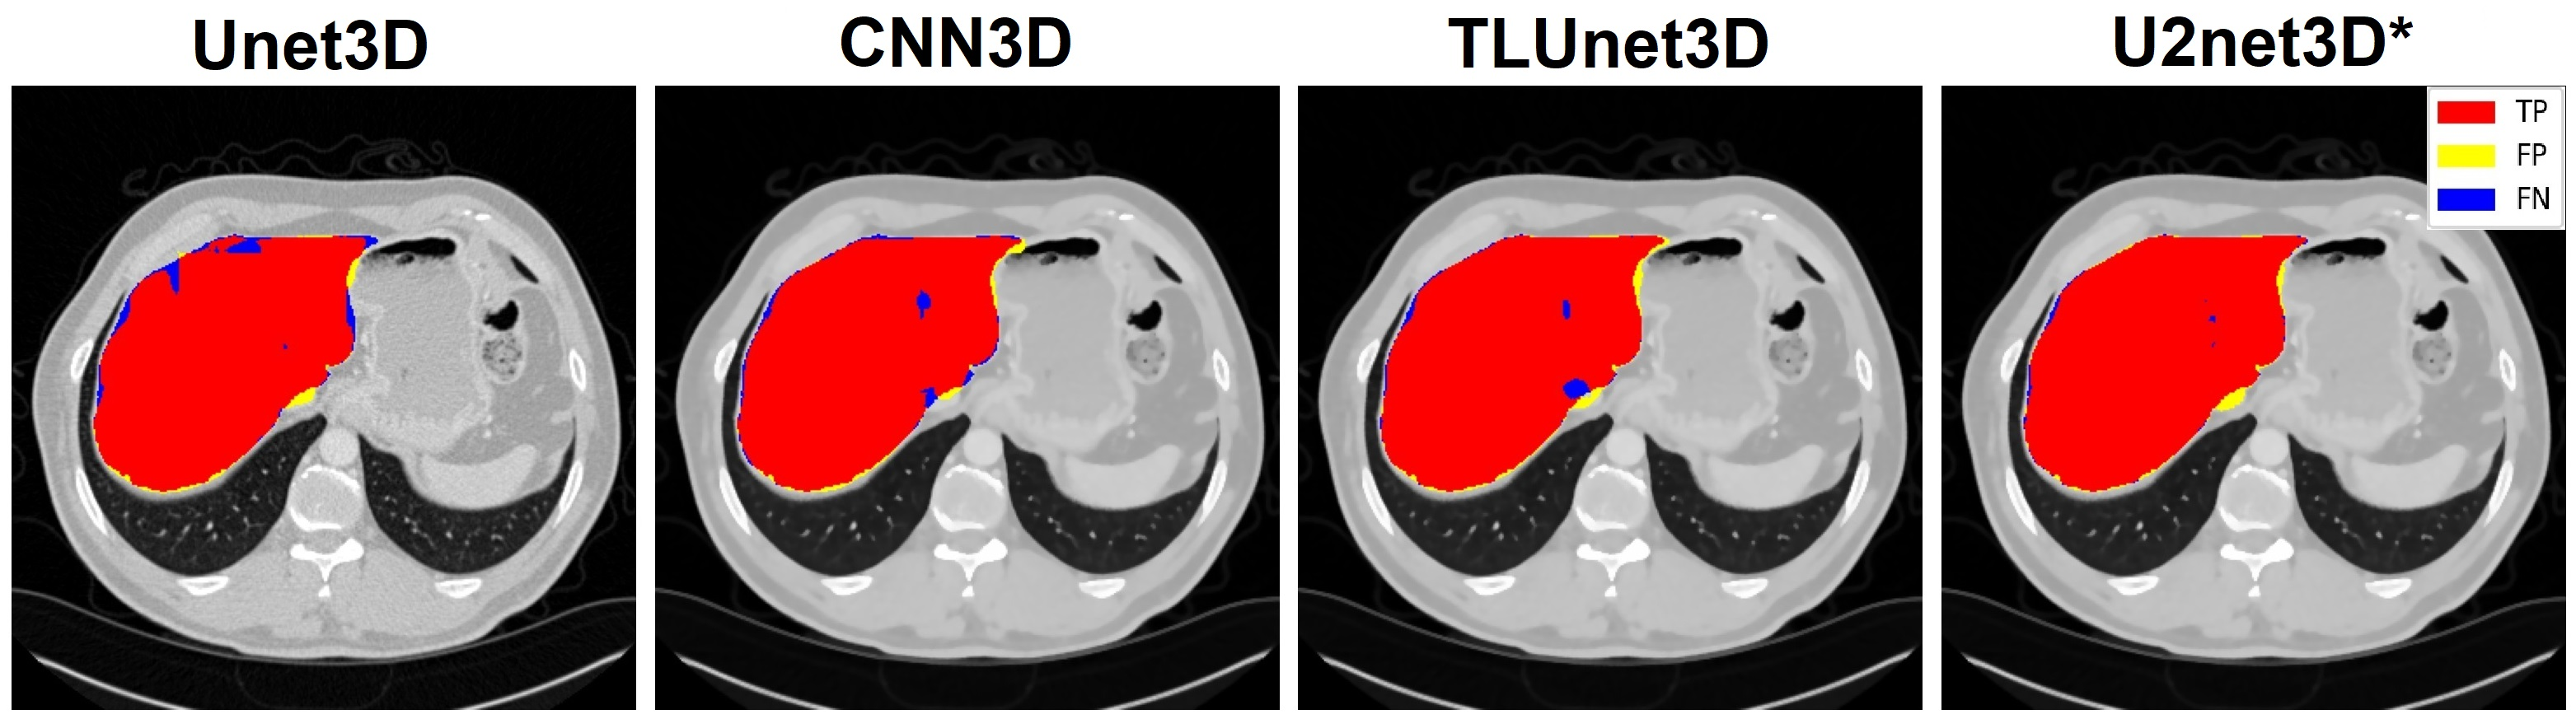
\includegraphics[width=\textwidth]{images/liver/U2Net3D/liver-result-legend.jpg}
    \caption{Kết quả dự đoán một mẫu dữ liệu trên tập Sliver07.}
    \label{fig:u2net3d-liver-result}
\end{figure}
\vspace{-5mm}
Hình \ref{fig:u2net3d-liver-result} minh họa kết quả dự đoán trên một lát cắt trên tập Sliver07 của các mô hình. Nhìn chung, các mô hình đều cho kết quả phân đoạn khá sát với thực tế, chỉ một vài phần nhỏ chưa phân đoạn được. Mô hình U2net3D* cho kết quả phần nền dự đoán sai (màu xanh) ít hơn các mô hình còn lại.
\subsection{Phân đoạn mạch máu}
Đối với bài toán phân đoạn mạch máu, mô hình đề xuất U2net3D* đã đạt được sự cải tiến lớn. Hệ số tương đồng (Dice) tăng 4\% (từ \textbf{ 56,29\%} lên đến \textbf{60.75\%}). Mặc dù độ chính xác có giảm bởi tỷ lệ dự đoán nhầm tăng nhưng độ phủ (Recall) cải thiện đáng kể.

\begin{table}[H]
    \renewcommand{\arraystretch}{1.1}
    \centering
    \begin{tabular}{c l c c c}
        \Xhline{2\arrayrulewidth}
        \multirow{2}{*}{\textbf{STT}} & \multirow{2}{*}{\textbf{Mô hình}} & \multicolumn{3}{c}{\textbf{Tập kiểm tra}} \\ \cline{3-5}
        & &  \textbf{Dice} & \textbf{Recall} & \textbf{Precision} \\ 
        \Xhline{2\arrayrulewidth}
        1   & Unet2D\cite{Unet}      & 41.17 & 60.05 & 31.32\\
        2   & Unet3D\cite{LV_LIVER}       & 56.29 & 44.27 & \textbf{73.97} \\
        3   & CNN3D\cite{LV_VESEL}        & 54.26 & 54.98 & 59.16 \\
        4   & U2net3D*     & \textbf{60.75} & \textbf{66.87} & 59.73 \\
        \Xhline{2\arrayrulewidth}
    \end{tabular}
    \caption{Kết quả phân đoạn mạch máu của các mô hình (\%).}
\end{table}

Để đánh giá một cách chi tiết các mẫu dữ liệu trong tập kiểm tra, chúng tôi đã tiến hành đánh giá trên từng bệnh nhân như sau. Mặc dù tập kiểm tra chỉ có 3 bệnh nhân tuy nhiên, trong quá trình huấn luyện mô hình chúng tôi không sử dụng toàn bộ 1 volume của 1 bệnh nhân để forward qua một lần mà sử dụng các khối sub-volume nhỏ hơn được sinh ra từ volume ban đầu. Do đó mặc dù chỉ chứa 3 bệnh nhân nhưng số lượng mẫu được lan truyền qua mạng cũng có số lượng đủ lớn (khoảng 350 sub-volume có kích thước 64$\times$96$\times$96) để đánh giá hiệu quả của mô hình. 
\begin{table}[H]
    \renewcommand{\arraystretch}{1.1}
    \centering
    \begin{tabular}{c l c c c}
        \Xhline{2\arrayrulewidth}
        \multirow{2}{*}{\textbf{STT}} & \multirow{2}{*}{\textbf{Bệnh nhân}} & \multicolumn{3}{c}{\textbf{Tập kiểm tra}} \\ \cline{3-5}
        & &  \textbf{Dice} & \textbf{Recall} & \textbf{Precision} \\ 
        \Xhline{2\arrayrulewidth}
        1   & Bệnh nhân số 1 & 50.73 & \textbf{82.85} & 36.55\\
        2   & Bệnh nhân số 6 & 62.52 & 65.66 & 59.76 \\
        3   & Bệnh nhân số 11 & \textbf{68.79} & 64.09 & \textbf{74.23} \\
        \Xhline{2\arrayrulewidth}
    \end{tabular}
    \caption{Kết quả phân đoạn mạch máu chi tiết các bệnh nhân trong tập kiểm tra(\%).}
    \label{tab:vessel-result-patient}
\end{table}

Dựa vào bảng \ref{tab:vessel-result-patient} có thể thấy được bệnh nhân số 6 và bệnh nhân số 11 cho kết quả rất tốt, hơn nữa 2 độ đo Recall và Precision khá tương đồng. Tuy nhiên khi đánh giá bệnh nhân số 0 thuộc trường hợp xấu nhất, điều này có thể giải thích được bởi việc thiếu dữ liệu huấn luyện. Nhắc lại quy trình chia dữ liệu được đề cập ở chương 4 bảng \ref{tab:training-set-vessel}, có thể thấy bệnh nhân số 1 thuộc nhóm dữ liệu có giá trị Hounsfield Unit trung bình cao nhất trong 3 nhóm. Đặc biệt hơn nhóm này chỉ có 2 bệnh nhân để đưa vào huấn luyện. Do đó có thể kết luận được việc tại sao bệnh nhân số 1 này lại đưa ra kết quả tệ nhất, bởi việc không đủ dữ liệu có thể đại diện cho mẫu này do đó mô hình vẫn chưa có khả năng dự đoán 1 cách chính xác nhất nếu rơi vào trường hợp này. Sau đây là histogram biễu diễn phân phối Hounsfield Unit của 3 bệnh nhân trong tập kiểm tra.

\begin{figure}[H]
    \centering
    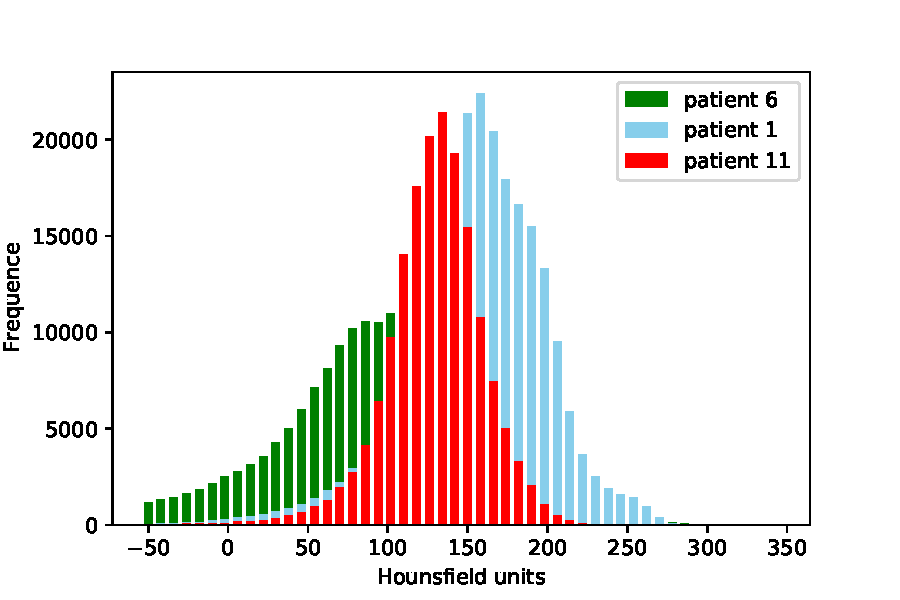
\includegraphics[width=.7\textwidth]{images/blood/test_hist.pdf}
    \caption{Phân phối Hounsfield Unit của các bệnh nhân trong tập kiểm tra.}
\end{figure}

Có thể thấy phân bố các giá trị hounsfield unit của bệnh nhân 1 phân bố ở vùng có giá trị cao hơn các bệnh nhân còn lại. Sau đây là kết quả trực quan của từng bệnh nhân:

\begin{figure}[H]
    \centering
    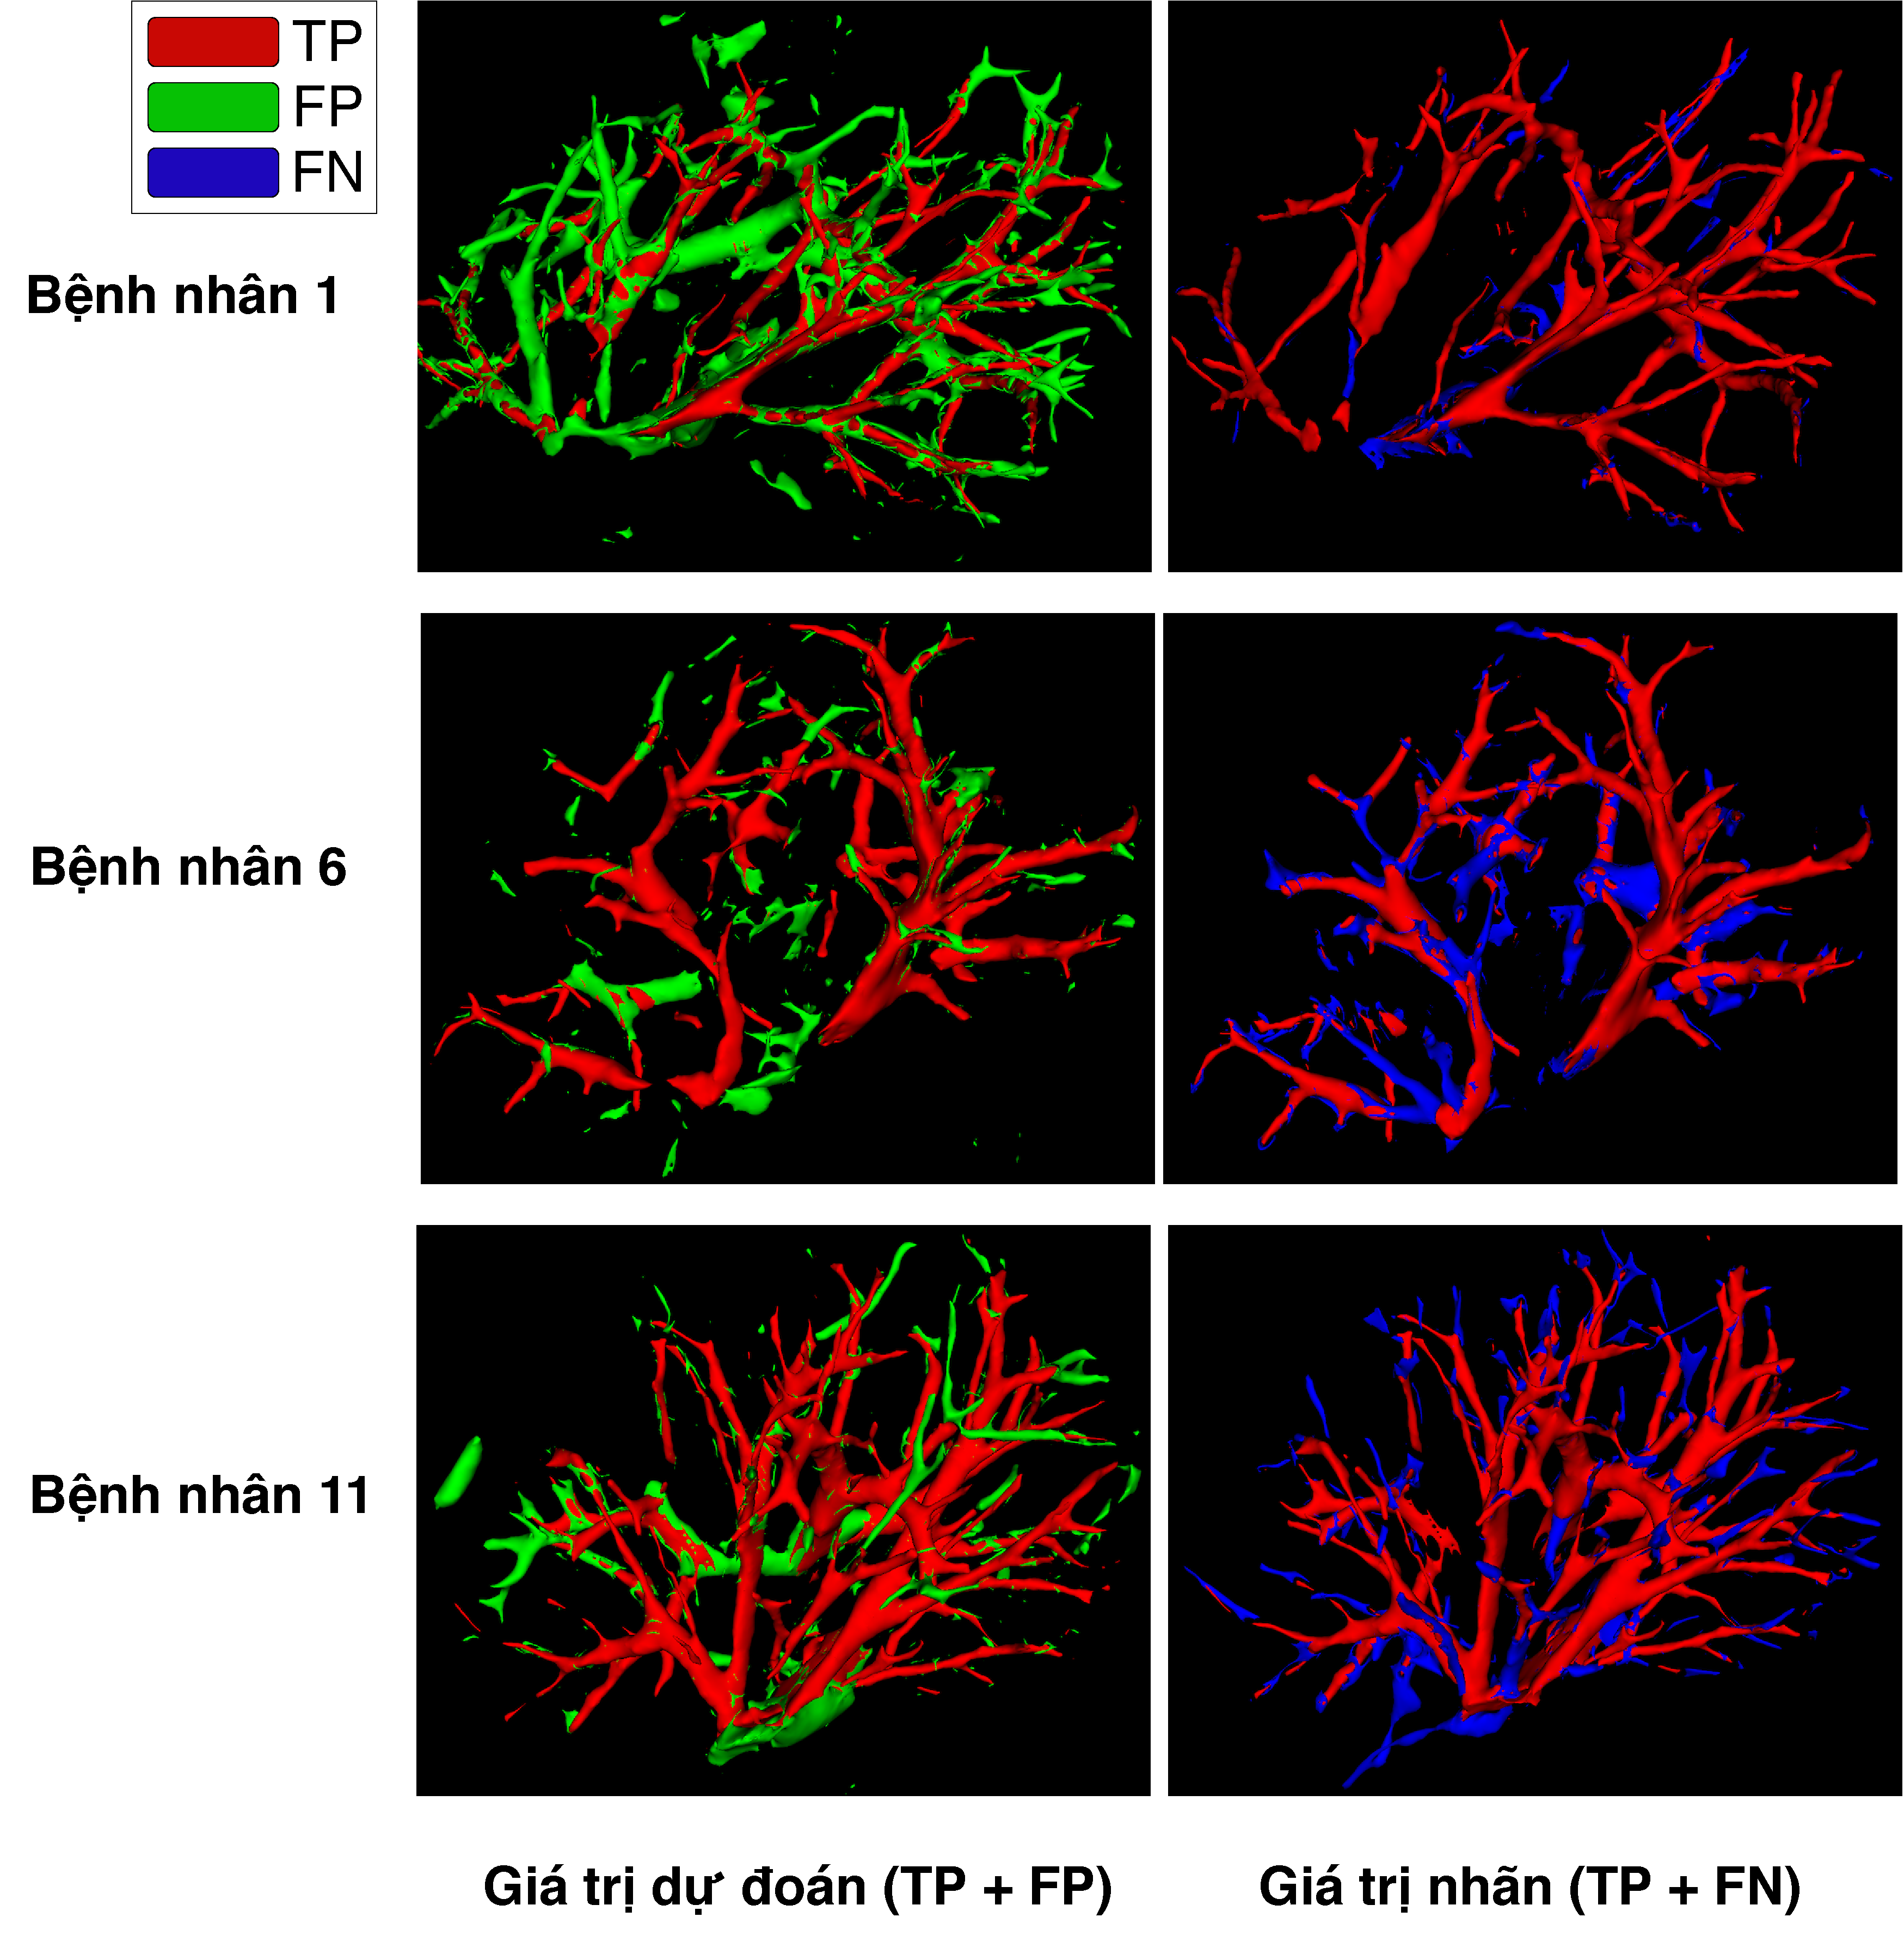
\includegraphics[width=\textwidth]{images/blood/3d_vessel.pdf}
    \caption{Kết quả trực quan hóa dưới dạng 3D của từng bệnh nhân.}
    \label{fig:3d-vessel}
\end{figure}

Dựa vào hình \ref{fig:3d-vessel} cho thấy được bệnh nhân 1 có kết quả dự đoán khá là nhiễu bởi mẫu này cho ra độ precision thấy, tuy nhiên độ recall lại cao nhất trong 3 bệnh nhân nên vùng màu xanh dương khá là ít. Trong khi đó 2 bệnh nhân còn lại cho ra kết quả khá tương đồng với mạch máu thật, ít bị nhiễu bởi False Positive hơn.

	\chapter{HỆ THỐNG LÀM NHÃN ẢNH Y KHOA DAT}\label{chapter:architecture}

\section{Mục tiêu của hệ thống DAT}
Để đáp ứng nhu cầu làm nhãn ảnh y khoa phục vụ cho việc huấn luyện mạng học sâu, nhóm chúng tôi đã kế thừa và phát triển hệ thống DAT (Data Annotation Tool) của phòng lab Computer Vision and Graphics. DAT là một công cụ làm nhãn dữ liệu đặc thù cho ảnh DICOM. \\
\indent Bài toán phân đoạn ảnh y khoa dùng mạng học sâu luôn cần một số lượng dữ liệu lớn. Nguồn dữ liệu dồi dào và chính xác là một trong những yếu tố giúp việc huấn luyện mạng hiệu quả hơn. Việc gán nhãn dữ liệu, đặc biệt là những tập dữ liệu đặc thù như ảnh y khoa cần có một công cụ hỗ trợ hợp lý. Nhận thức được nhu cầu này, nhóm đã cải thiện hệ thống DAT với nhiều chức năng phù hợp cho việc gán nhãn ảnh DICOM.

\section{Phân tích yêu cầu}
\subsection{Quản trị hệ thống và dữ liệu}
\noindent- Quản lý người dùng:  Hệ thống DAT cho phép người quản trị thực hiện thao tác thêm mới và cấu hình vai trò của người dùng. \\
- Quản lý dữ liệu: 
\begin{itemize}
    \item Chức năng tải lên dữ liệu làm nhãn: Dữ liệu ảnh DICOM cần lãm nhãn sẽ được tải lên ở dạng .ZIP. Sau đó, dữ liệu sẽ được Django server đẩy tới và lưu trữ tại server orthanc.
    \item Chức năng cấu hình nhãn: Thêm mới một loại nhãn cần làm cho đối tượng dữ liệu. Ví dụ nhãn gan, nhãn mạch máu, nhãn khối u. 
    \item Chức năng cấu hình dữ liệu ảnh y khoa để làm nhãn: Cho phép người quản trị chọn tệp ảnh y khoa cần làm nhãn và chọn người làm nhãn trong số những người dùng. 
\end{itemize}
\subsection{Chức năng làm nhãn}
\begin{itemize}
    \item Tải và hiển thị ảnh y khoa trên giao diện, cho phép điều chỉnh ảnh theo độ sáng để làm rõ từng đối tương cụ thể : gan, mạch máu, phổi .
    \item Vẽ nhãn với sự hỗ trợ của giải thuật tăng trưởng vùng (region growing) theo độ sáng của ảnh. 
    \item Vẽ nhãn bằng bút và vẽ nhãn tự do.
    \item Bật và tắt nhãn đang làm. 
    \item Xóa nhãn đang làm. 
    \item Hỗ trợ hai chế độ hiển thị vùng và hiển thị biên.
    \item Phóng to, thu nhỏ và kéo thả ảnh.
    \item Lưu nhãn xuống cơ sở dữ liệu.
    \item Sử dụng dự đoán AI để làm nhãn nhanh và chính xác hơn.
    \item Thao tác undo.
    \item Thao tác reset.
    \item Thao tác chuyển slice.
\end{itemize}

\section{Công nghệ sử dụng}
\subsection{Ngôn ngữ lập trình}
Hệ thống được hiện thực dựa trên hai ngôn ngữ lập trình chính: 
\begin{itemize}
    \item Server: Ngôn ngữ Python và framework Django. Mô hình học sâu được hiện thực, huấn luyện và triển khai bằng ngôn ngữ Python. Vì vậy, việc chọn Python và framework Django để hiện thực server là một lựa chọn hợp lý để tăng cường khả năng tích hợp dự báo AI vào hệ thống làm nhãn DAT. 
    \item Client: Ngôn ngữ Javascript và thư viện ReactJS. React là một thư viện UI phát triển tại Facebook để hỗ trợ việc xây dựng những thành phần (components) UI có tính tương tác cao, có trạng thái và có thể sử dụng lại được. Javascript có nhiều thư viện hỗ trợ việc thao tác trên ảnh y khoa như thư viện Cornerstone.js. 
\end{itemize}

\subsubsection{Python}
% \begin{figure}[H]
%     \centering
%     
\includegraphics[width=7cm]{images/chapter-07-images/python-programming.png}
%     \caption{Ngôn ngữ lập trình Python}
% \end{figure}
Python là một ngôn ngữ lập trình thông dịch, hướng đối tượng, cấp cao với ngữ nghĩa động do Guido van Rossum tạo ra và lần đầu ra mắt vào năm 1991. \\
\indent Lý do chọn ngôn ngữ lập trình python: Thứ nhất, hệ thống DAT được xây dựng dựa trên framework Django - một web framework được viết bằng python. Thứ hai, mô hình mạng học sâu do nhóm huấn luyện trên framework pytorch. Vì vậy, việc tích hợp  dự báo AI từ mô hình mạng học sâu vào hệ thống làm nhãn DAT sẽ thuận tiện hơn rất nhiều. 

\subsubsection{Javascript}
% \begin{figure}[H]
%     \centering
%     
\includegraphics[width=7cm]{images/chapter-07-images/javascript-5.png}
%     \caption{Ngôn ngữ lập trình Javascript}
% \end{figure}
JavaScript là một ngôn ngữ lập trình dạng scripting cho phép bạn triển khai các tính năng phức tạp trên các trang web. \\
\indent Lý do chọn ngôn ngữ lập trình javascript: Với thư viện Reactjs hỗ  trợ mạnh mẽ cho việc xây dựng front-end cho hệ thống, cùng một số thư viện khác phục vụ cho việc thao tác trên ảnh DICOM ở phía client ví dụ thư viện Cornerstone.js.
\subsection{Thư viện và frameworks}
\subsubsection{Django}
% \begin{figure}[H]
%     \centering
%     
\includegraphics[width=7cm]{images/chapter-07-images/django-logo-negative.png}
%     \caption{Web framework Django}
% \end{figure}
Django là một web framework bật cao được viết bằng Python, cho phép phát triển ứng dụng nhanh chóng, gọn gàng. Django đã giải quyết rất nhiều rắc rối trong quá trình phát triển web, giúp người dùng tập trung vào việc phát triển ứng dụng với châm ngôn "không cần phát minh lại bánh xe".\\
\indent Nhóm dựa trên kiến trúc mô hình MVT của Django để xây dựng hệ thống DAT, chi tiết sẽ được trình bày ở phần kiến trúc hệ thống. 

\subsubsection{ReactJS}
% \begin{figure}[H]
%     \centering
%     
\includegraphics[width=7cm]{images/chapter-07-images/react-js-logo.png}
%     \caption{Thư viện ReactJS}
% \end{figure}
ReactJS là một thư viện Javascript được sử dụng trong quá trình phát triển web để xây dựng những phần tử tương tác trên website. React sử dụng khái niệm Virtual DOM, Virtual DOM tạo ra bản cache cấu trúc dữ liệu của ứng dụng trên bộ nhớ. Với mỗi lượt thay đổi, React chỉ render lại những component thực sự thay đổi, việc này giúp tăng tốc độ phản hồi của ứng dụng một cách hiệu quả.\\
\indent Nhóm sử dụng thư viện ReactJS kết hợp với Material-UI để xây dựng phần front-end cho hệ thống DAT, chi tiết sẽ được trình bày ở phần kiến trúc hệ thống. 

\subsubsection{Material-UI}
% \begin{figure}[H]
%     \centering
%     
\includegraphics[width=7cm]{images/chapter-07-images/material-ui-logo.png}
%     \caption{Material - UI}
% \end{figure}
Material-UI là một ngôn ngữ thiết kế được Google phát triển vào năm 2014. Với lượng component được thiết kế sắn rất đẹp mắt, tài liệu hướng dẫn dầy đủ, Material-UI là một lựa chọn hấp nhẫn cho bất kỳ nhà phát triển website nào.

\subsection{Cơ sở dữ liệu}

% \begin{figure}[H]
%     \centering
%     
\includegraphics[width=7cm]{images/chapter-07-images/postgresql-la-gi.png}
%     \caption{Hệ quản trị cơ sở dữ liệu PostgreSQL}
% \end{figure}

PostgreSQL là một hệ thống quản trị cơ sở dữ liệu quan hệ miễn phí và nguồn mở (RDBMS) tập trung vào khả năng mở rộng và tuân thủ các tiêu chuẩn kỹ thuật. Nó được thiết kế để xử lý một loạt các khối lượng công việc lớn, từ các máy tính cá nhân đến kho dữ liệu hoặc dịch vụ Web có nhiều người dùng đồng thời.

PostgreSQL bắt đầu từ năm 1986 như một phần của dự án POSTGRES tại Đại học California tại Berkeley và có hơn 30 năm phát triển. Đây là cơ sở dữ liệu mặc định cho macOS Server, và cũng có các bản phân phối cho Linux, FreeBSD, OpenBSD và Windows.

\subsection{Công cụ, phần mềm hỗ trợ}

\subsubsection{Webpack}
% \begin{figure}[H]
%     \centering
%     
\includegraphics[width=7cm]{images/chapter-07-images/webpack-logo.png}
%     \caption{Webpack}
% \end{figure}
Về cốt lõi, webpack là một gói mô-đun tĩnh cho các ứng dụng JavaScript hiện đại. Khi webpack xử lý ứng dụng, nó xây dựng nội bộ một biểu đồ phụ thuộc ánh xạ mọi mô-đun mà dự án của bạn cần và tạo một hoặc nhiều gói.

\subsubsection{Nginx}
% \begin{figure}[H]
%     \centering
%     
\includegraphics[width=7cm]{images/chapter-07-images/NGINX-logo-rgb-large.png}
%     \caption{Nginx}
% \end{figure}

NGINX, đọc là “engine-ex,”  là một phần mềm web server mã nguồn mở nỗi tiếng. Ban đầu nó dùng để phục vụ web HTTP. Tuy nhiên, ngày nay nó cũng được dùng làm reverse proxy, HTTP load balancer và email proxy như IMAP, POP3, và SMTP.

NGINX xuất bản chính thức vào tháng 10 năm 2004. Nhà sáng lập của phần mềm này là Igor Sysoev, triển khai dự án từ năm 2002 để giải quyết vấn đề C10k. C10k là giới hạn của việc xử lý 10 ngàn kết nối cùng lúc. Ngày nay, có nhiều web server còn phải chịu nhiều kết nối hơn vậy để xử lý. NGINX sử dụng kiến trúc hướng sự kiện (event-driven) không đồng bộ (asynchronous). Tính năng này khiến NGINX server trở nên đáng tin cậy, tốc độ và khả năng mở rộng lớn nhất.

Vì khả năng mạnh mẽ, và để có thể xử lý hàng ngàn kết nối cùng lúc, nhiều website có traffic lớn đã sử dụng dịch vụ NGINX. Một vài trong số những ông lớn công nghệ dùng nó là Google, Netflix, Adobe, Cloudflare, WordPress, và còn nhiều hơn nữa.


\subsubsection{Docker}
% \begin{figure}[H]
%     \centering
%     
\includegraphics[width=7cm]{images/chapter-07-images/docker-logo.png}
%     \caption{Docker}
% \end{figure}
Docker là một nền tảng cho developers và sysadmin để develop, deploy và run application với container. Nó cho phép tạo các môi trường độc lập và tách biệt để khởi chạy và phát triển ứng dụng và môi trường này được gọi là container. Khi cần deploy lên bất kỳ server nào chỉ cần run container của Docker thì application của bạn sẽ được khởi chạy ngay lập tức.

\subsubsection{Orthanc - DICOM Server}
% \begin{figure}[H]
%     \centering
%     
\includegraphics[width=7cm]{images/chapter-07-images/orthanc-logo.png}
%     \caption{Orthanc DICOM Server}
% \end{figure}
Orthanc cung cấp một máy chủ DICOM để lưu trữ ảnh y khoa. Orthanc cho phép người dùng tập trung vào nội dung các tệp ảnh DICOM, đơn giản hóa sự phức tạp của định dạng ảnh. Orthanc hoạt động được trên Linux, Windows, có kiến trúc nhẹ và độc lập, không phụ thuộc nhiều vào bên thứ ba.\\
Với hệ thống DAT này, chúng tôi chạy Orthanc - DICOM Server trong môi trường docker dựa trên một docker image có tên là jodogne/orthanc-plugins. 

\section{Kiến trúc hệ thống}
\subsection{Tổng quan kiến trúc hệ thống}
\begin{figure}[H]
    \centering
    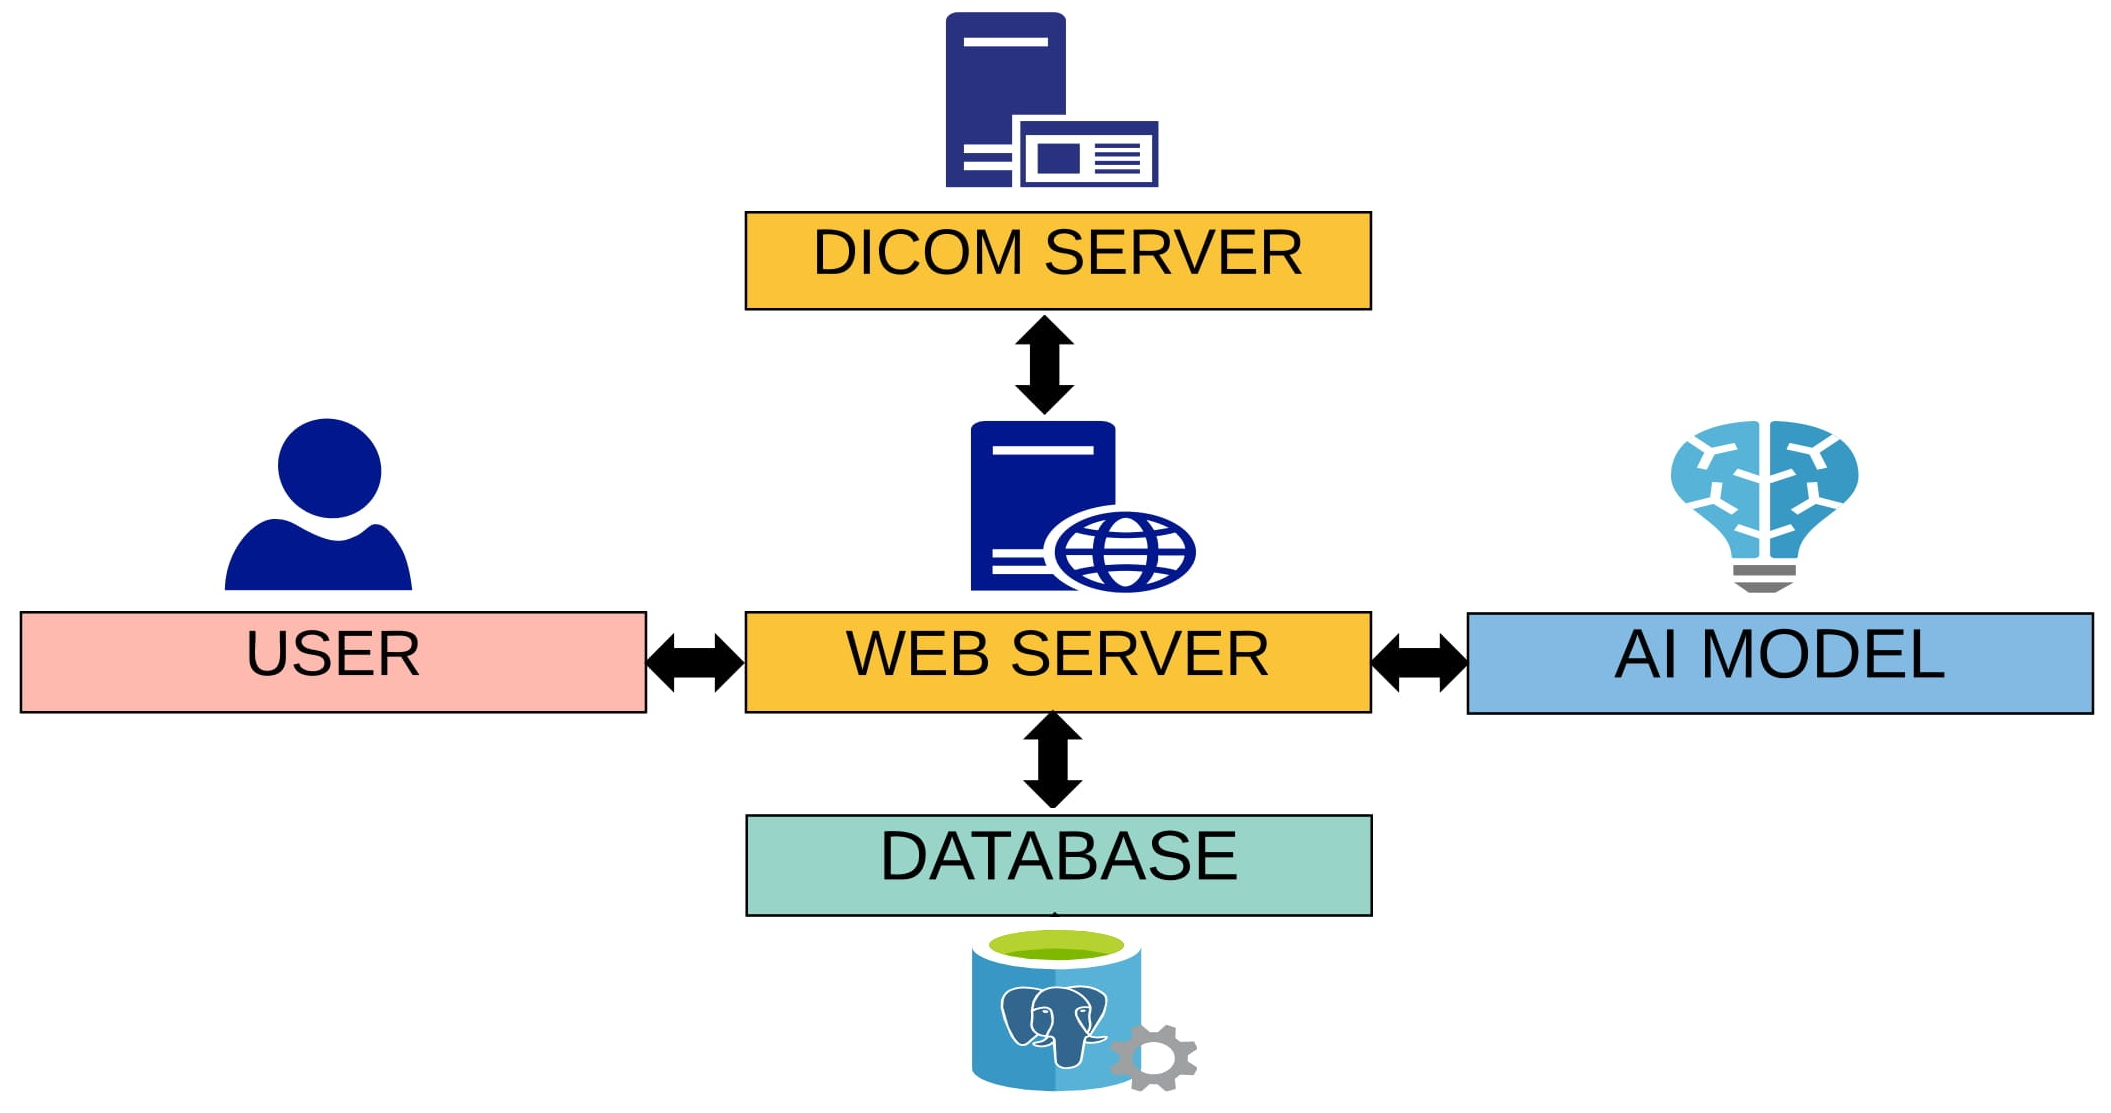
\includegraphics[width=14cm]{images/chapter-07-images/mvt-1.jpg}
    \caption{Tổng quan kiến trúc hệ thống DAT}
\end{figure}
Hệ thống DAT được xây dựng dựa trên mô hình MVT (Model - View - Template) của framework Django kết hợp với mô hình dự báo nhãn (AI MODEL).  

\begin{itemize}
    \item Model: Đây là phần trung gian chịu trách nhiệm xử lý dữ liệu giữa phần view (hiển thị cho người dùng) và phần cơ sở dữ liệu PostgreSQL. Model định nghĩa cấu trúc dữ liệu được lưu trữ cho phần dữ liệu đến từ View và truy xuât thông tin từ cơ sử dữ liệu, trả về cho View ở dạng xem được. Mỗi Model trong Django tương ứng với một bảng trong cơ sử dữ liệu. 
    \item View: Chịu trách nhiệm cho những gì người dùng thấy ở phía client. Một hàm view trong mô hình Django là một hàm Python nhận yêu cầu (“POST”,”GET”) từ phía người dùng và trả về một web response, response này có thể là nội dung HTML của trang web, một chuyển trang, một hình ảnh hoặc một response ở dạng JSON. 
    \item Template: Là phần thứ ba trong mô hình MVT, Template được viết bằng HTML, CSS và Javascript trong một file .html. Template cung cấp bố cục và giao diện trang web cho người dùng.
    \item Orthanc Server: Là nơi lưu trữ ảnh y khoa phục vụ việc lãm nhãn dữ liệu. 
    \item AI Model: Để việc làm nhãn được thuận tiện, nhanh chóng và chính xác hơn, AI Model được tích hợp vào hệ thống DAT. AI Model được chạy trong Django server và chịu trách nhiệm nhận yêu cầu từ phía client và trả về kết quả dự đoán. 
\end{itemize}

\subsection{Chi tiết kiến trúc hệ thống}
\subsubsection{Sơ đồ use case}
\begin{figure}[H]
    \centering
    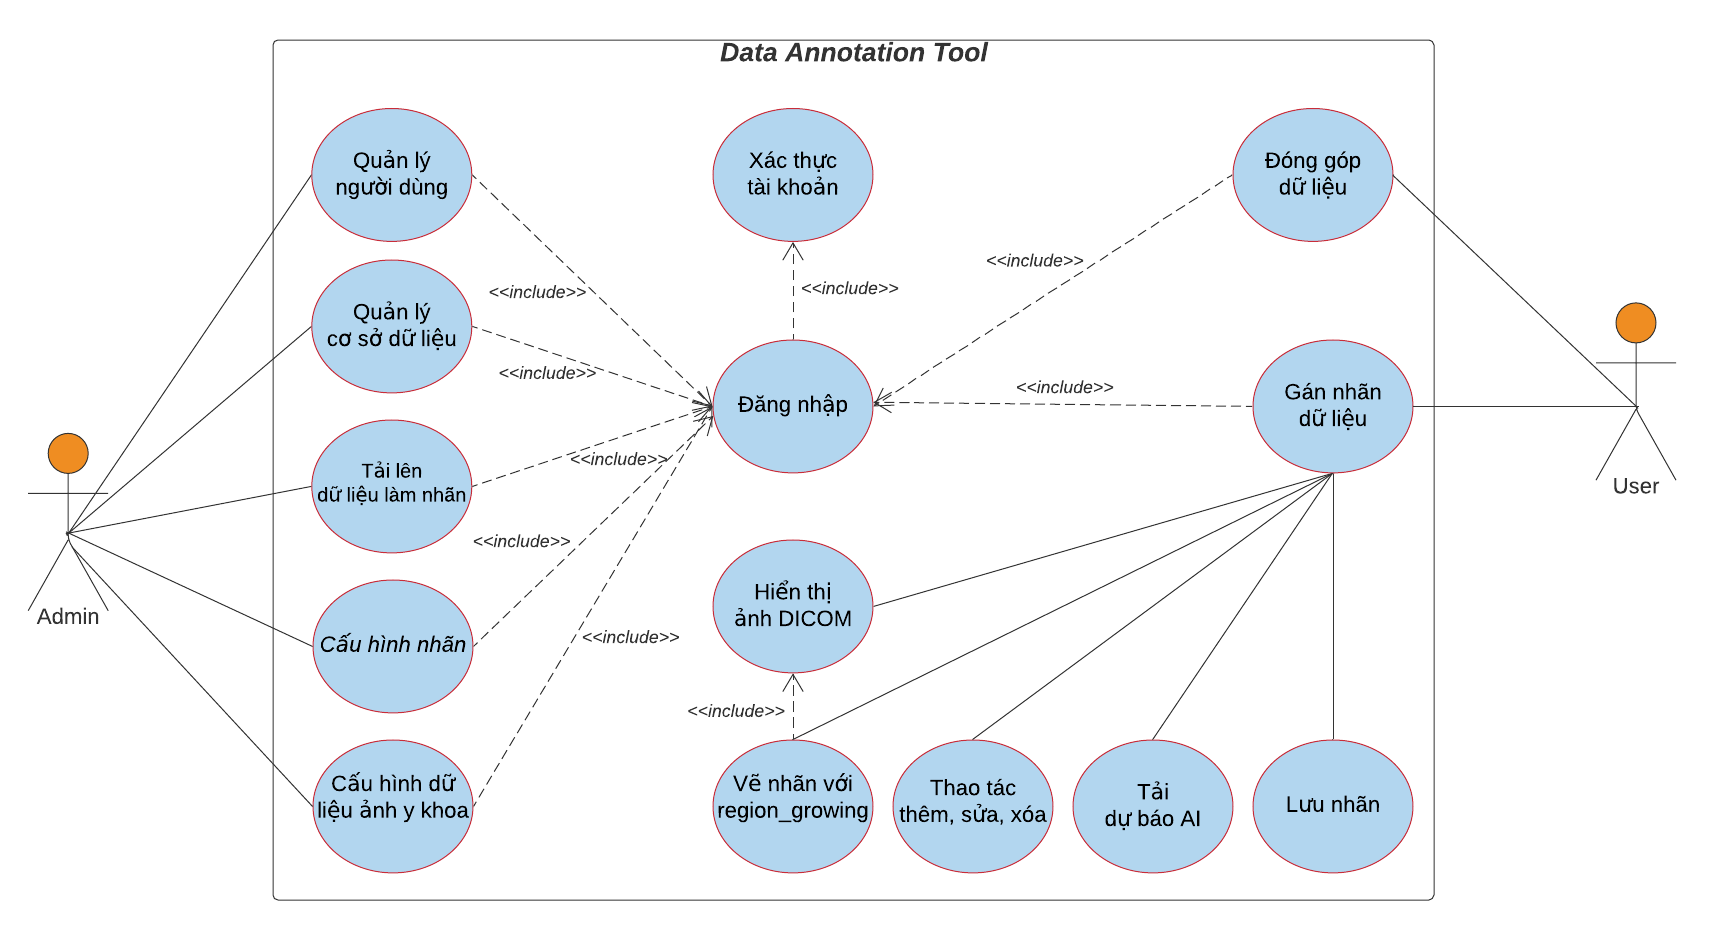
\includegraphics[width=14cm]{images/chapter-07-images/use-case-dat.png}
    \caption{Sơ đồ use case hệ thống DAT}
\end{figure}

\subsubsection{Sơ đồ sequence diagram}
\begin{figure}[H]
    \centering
    \includegraphics[width=14cm]{images/chapter-07-images/sequence-diagram.png}
    \caption{Sơ đồ sequence diagram hệ thống DAT}
\end{figure}

\subsubsection{Thiết kế cơ sở dữ liệu với Django Models}
Framework Django hỗ trợ lớp model để người dùng tương tác với cơ sở dữ liệu, mỗi model là một bảng gồm những trường được mô tả và quan hệ với các model khác (nếu có). Với hệ thống DAT này, ngoài những bảng dữ liệu được kế thừa, chúng tôi thiết kế thêm hai bảng dữ liệu chính:
\begin{itemize}
    \item Bảng dữ liệu để lưu nhãn đã làm: Sau khi bước làm nhãn kết thúc, dữ liệu nhãn sẽ được lưu trong bảng này, có thể xuất ra file .csv.
    \item Bảng dữ liệu để lưu nhãn được dự đoán bằng AI: Với một tập dữ liệu mới, người dùng có thể chạy dự đoán AI để hỗ trợ việc làm nhãn. Sau lần chạy dự đoán AI đầu tiên, phần nhãn được AI dự đoán sẽ được lưu vào bảng dữ liệu này để phục vụ việc làm nhãn. 
\end{itemize}


\begin{figure}[H]
    \centering
    \includegraphics[width=17cm]{images/chapter-07-images/data-base-version-4.pdf}
    \caption{Thiết kế cơ sở dữ liệu với Django Model}
\end{figure}


\subsubsection{Cấu trúc mã nguồn hệ thống}
\begin{figure}[H]
    \centering
    \includegraphics[width=14cm]{images/chapter-07-images/source-code-system.png}
    \caption{Cấu trúc mã nguồn hệ thống DAT}
\end{figure}


\section{Đặc tả tính năng hệ thống}
\newpage
\subsection{Tổng quan luồng hoạt động của hệ thống}
\begin{figure}[H]
    \centering
    \includegraphics[width=16cm]{images/chapter-07-images/flow-chart-no-05.png}
    \caption{Luồng hoạt động hệ thống DAT}
\end{figure}


Flowchart với vai trò người quản trị

Flowchart với vai trò người dùng làm nhãn

\subsection{Chức năng đăng nhập và xác thực người dùng}
Hệ thống DAT hỗ trợ 2 vai trò đăng nhập khác nhau, một cho người quản trị hệ thống, hai cho người dùng làm nhãn. Với vai trò thứ nhất, sau khi đăng nhập thành công, người quản trị được phép thực hiện quản lý người dùng, quản lý dữ liệu làm nhãn, cấu hình nhãn và chỉ định người dùng lãm nhãn. Với vai trò thứ hai, sau khi đăng nhập, người dùng có thể  làm nhãn dữ liệu ảnh y khoa trên những tập dữ liệu đã được người quản trị chỉ định. 
\begin{figure}[H]
    \centering
    \includegraphics[width=14cm]{images/chapter-07-images/ui-dang-nhap.png}
    \caption{Giao diện đăng nhập của hệ thống DAT}
\end{figure}
\begin{figure}[H]
    \centering
    \includegraphics[width=14cm]{images/chapter-07-images/ui-dang-nhap-admin.png}
    \caption{Giao diện đăng nhập với vai trò admin của hệ thống DAT}
\end{figure}
\begin{figure}[H]
    \centering
    \includegraphics[width=14cm]{images/chapter-07-images/ui-dang-nhap-user.png}
    \caption{Giao diện đăng nhập với vai trò admin của hệ thống DAT}
\end{figure}

\subsection{Chức năng tải lên tập dữ liệu làm nhãn}
Hệ thống DAT cung cấp giao diện này để người quản trị tải lên tập dữ liệu ảnh y khoa cần làm nhãn. Tập tin được tải lên ở định dạng nén (.zip). Sau khi tải lên tập dữ liệu ảnh y khoa, người quản trị chọn mục "is medical image", đồng thời chỉ định chủ sở hữu dữ liệu và thêm phần mô tả ở bên dưới. Cuối cùng, người quản trị chọn lưu và có thể thoát hoặc tải lên tập dữ liệu khác.

\begin{figure}[H]
    \centering
    \includegraphics[width=14cm]{images/chapter-07-images/admin-input-data-model-1.png}
    \caption{Giao diện đăng nhập với vai trò admin của hệ thống DAT}
\end{figure}

\begin{figure}[H]
    \centering
    \includegraphics[width=14cm]{images/chapter-07-images/admin-input-data-model-2.png}
    \caption{Giao diện đăng nhập với vai trò admin của hệ thống DAT}
\end{figure}

\subsection{Chức năng cấu hình tập dữ liệu ảnh y khoa và chỉ định người lãm nhãn}
Để cấu hình tập dữ liệu ảnh y khoa, hệ thống DAT cung cấp mục \textbf{\textit{Medical data set model}}. Người quản trị bấm chọn tập dữ liệu cần cấu hình, sau đó chọn 4 thì tương ứng bao gồm: thì không thuốc, thì động mạch, thì tĩnh mạch và thì muộn. Tiếp tục chọn loại nhãn cần làm trên tập dữ liệu này, đồng thời chỉ định người làm nhãn và bấm nút lưu. 
\begin{figure}[H]
    \centering
    \includegraphics[width=14cm]{images/chapter-07-images/admin-medical-dataset-model-1.png}
    \caption{Giao diện đăng nhập với vai trò admin của hệ thống DAT}
\end{figure}
\begin{figure}[H]
    \centering
    \includegraphics[width=14cm]{images/chapter-07-images/admin-input-data-model-2.png}
    \caption{Giao diện đăng nhập với vai trò admin của hệ thống DAT}
\end{figure}


\subsection{Chức năng làm nhãn dữ liệu y khoa}
Sau khi đăng nhập thành công, những tập dữ liệu nào đã được người quản trị chỉ định sẽ hiện trên giao diện chính của người dùng. Người dùng tiến hành bấm chọn tập dữ liệu cần thao tác và sau đó  bắt đầu làm nhãn. \\
\indent Hệ thống DAT hỗ  trợ dự đoán AI cho tập dữ liệu ảnh y khoa cần làm nhãn, giúp quá trình làm nhãn nhanh và tiện lợi hơn. Ngoài ra, hệt thống DAT còn hỗ trợ làm nhãn với giải thuật tăng trưởng vùng theo độ sáng, vẽ bằng bút, xóa, undo,...\\
\indent Phân giao diện chính với thanh menu bên trái và phần làm nhãn tương ứng với bốn thì (không thuốc, động mạch, tĩnh mạch và thì muộn) của ảnh DICOM bên phải. 

\begin{figure}[H]
    \centering
    \includegraphics[width=\textwidth]{images/chapter-07-images/user-ui-medical-labeling.png}
    \caption{Tổng quan giao diện làm nhãn ảnh DICOM}
\end{figure}

\begin{figure}[H]
    \centering
    \includegraphics[width=\textwidth]{images/chapter-07-images/ui-labeling-13.png}
    \caption{Chi tiết giao diện làm nhãn ảnh DICOM}
\end{figure}

Để việc làm nhãn thuận lợi và nhanh chóng hơn, người dùng có thể chạy dự đoán AI (hiện lên nhãn màu đỏ).
\begin{figure}[H]
    \centering
    \includegraphics[width=\textwidth]{images/chapter-07-images/user-non-contrast-demo.png}
    \caption{Dự đoán AI cho phần làm nhãn ở thì không thuốc (Non contrast phase)}
\end{figure}

Để vẽ nhãn, người dùng có thể chọn chế  độ vẽ bằng bút, vẽ tự do hoặc vẽ với giải thuật tăng trưởng vùng theo mức sáng.
\begin{figure}[H]
    \centering
    \includegraphics[width=\textwidth]{images/chapter-07-images/user-labeling-by-brush.png}
    \caption{Vẽ nhãn bằng bút trên ảnh DICOM ở thì không thuốc}
\end{figure}

\begin{figure}[H]
    \centering
    \includegraphics[width=\textwidth]{images/chapter-07-images/ui-labeling-region-growing.png}
    \caption{Vẽ nhãn với giải thuật tăng trưởng vùng trên ảnh DICOM ở thì không thuốc}
\end{figure}

\begin{figure}[H]
    \centering
    \includegraphics[width=\textwidth]{images/chapter-07-images/ui-adjust-contrast.png}
    \caption{Điểu chỉnh độ sáng để  làm nổi bật đối tượng cần làm nhãn}
\end{figure}

\begin{figure}[H]
    \centering
    \includegraphics[width=\textwidth]{images/chapter-07-images/user-zoom-in.png}
    \caption{Phóng to một vùng trong ảnh DICOM}
\end{figure}


\section{Đánh giá và so sánh hệ thống DAT}
\subsection{Đánh giá hệ thống DAT}
\subsubsection{Ưu điểm}
\begin{itemize}
    \item Hỗ  trợ dự đoán AI vào phần ảnh DICOM cần làm nhãn, từ đó giảm thời gian làm nhãn đáng kể so với thông thường. Với những mô hình phân đoạn gan hiện tại, kết quả hệ số dice đều lớn hơn 90 phần trăm, vì vậy sau khi chạy dự đoán AI, người dùng chỉ cần thao tác rất ít để đạt được một nhãn chính xác.
    \item Giải thuật tăng trưởng vùng (region growing) theo độ sáng hỗ trợ làm nhãn nhanh, tiện lợi. 
    \item Có thể điều chỉnh độ sáng của ảnh để làm nổi bật  một số đối tượng cụ thể, ví dụ gan, mạch máu, phổi. 
    \item Cung cấp nhiều chế độ vẽ bao gồm vẽ nhãn bằng bút, vẽ nhãn bằng thao tác kéo thả chuột (free draw mode)
    \item Đồng bộ nhãn giữa 4 thì: thì không thuốc, thì động mạch, thì tĩnh mạch và thì muộn. 
    \item Hỗ trợ hai ngôn ngữ:  Tiếng Anh và tiếng Việt
    \item Có thể chuyển đổi giữa hai chế độ hiển thị nhãn: chế độ hiển thị vùng và chế độ hiển thị biên. 
    \item Có thể thực hiện thao tác quay về (undo) và xóa toàn bộ nhãn (reset to empty mask) nếu cần thiết. 
\end{itemize}

\subsubsection{Nhược điểm}
\begin{itemize}
    \item Hệ thống phản hồi chậm với các thao tác phòng to, thu nhỏ, kéo thả hình ảnh. Lý do: Một vùng cố định ROI (region of interest) sẽ được chọn để phóng to, thu nhỏ, kéo thả vì vậy sau mỗi lần thay đổi kích thước, hệ thống DAT sẽ tải và hiển thị lại vùng ROI này, dẫn đến việc UI phản hồi chậm. 
    \item Chưa thể tách riêng và thao tác độc lập trên  từng phần nhãn khi vẽ. 
\end{itemize}

\subsection{So sánh với hệ thống làm nhãn TrainingData.io}
TrainingData.io là công cụ làm nhãn ảnh y khoa được thành lập bởi một nhóm nhà phát triển giải pháp cho Visual AI có trụ sở tại San Francisco - Mỹ. \\

\begin{figure}[H]
    \centering
    \includegraphics[width=\textwidth]{images/chapter-07-images/user-training-data-io.png}
    \caption{Công cụ làm nhãn TrainingData.io}
\end{figure}

\indent Nhóm chúng tôi xin phép so sánh phần làm nhãn dữ liệu ảnh DICOM giữa hệ thống DAT do nhóm thừa kế và phát triển với hệ thống TrainingData.io dựa trên một số tiêu chí cơ bản như sau: 

% begin table - comparison table
\begin{table}[H]
\begin{tabular}{|l|c|c|}
\hline
\multicolumn{1}{|c|}{\textbf{Tiêu chí so sánh}}                                                                                   & \textbf{Data Annotation Tool} & \textbf{TrainingData.io} \\ \hline
\begin{tabular}[c]{@{}l@{}}Tải lên tập dữ liệu cần \\ làm nhãn\end{tabular}                                                       & có                            & có                       \\ \hline
\begin{tabular}[c]{@{}l@{}}Quản lý người dùng \\ làm nhãn\end{tabular}                                                            & có                            & có                       \\ \hline
Cấu hình nhãn                                                                                                                     & có                            & có                       \\ \hline
Dự đoán AI                                                                                                                        & có                            & có                       \\ \hline
\begin{tabular}[c]{@{}l@{}}Vẽ nhãn với giải thuật \\ tăng trường vùng\end{tabular}                                                & có                            & có                    \\ \hline
\begin{tabular}[c]{@{}l@{}}Phóng to, thu nhỏ, \\ kéo thả nhanh\end{tabular}                                                       & chậm                          & nhanh                    \\ \hline
\begin{tabular}[c]{@{}l@{}}Tách riêng và thao tác \\ độc lập trên từng phần \\ nhãn\end{tabular}                                  & không                         & có                       \\ \hline
\begin{tabular}[c]{@{}l@{}}Vẽ nhãn tự do với \\ chuột  (dạng đa giác)\end{tabular}                                                & có                            & có                       \\ \hline
Vẽ nhãn bằng bút vẽ                                                                                                               & có                            & không                    \\ \hline
\begin{tabular}[c]{@{}l@{}}Hỗ trợ tiếng Việt và \\ tiếng Anh\end{tabular}                                                         & có                            & chỉ hỗ trợ tiếng Anh     \\ \hline
\begin{tabular}[c]{@{}l@{}}Tùy chỉnh độ sáng để \\ làm nổi  bật một số đối \\ tượng  cụ thể (gan, mạch\\  máu, phổi)\end{tabular} & có                            & không                    \\ \hline
\end{tabular}
\caption{So sánh hệ thống DAT và hệ thống TrainingData.io}
\end{table}
% end table - comparison table 


\subsection{Hướng phát triển hệ thống trong tương lai}
Tử việc so sánh với một số công cụ làm nhãn ảnh y khoa hiện có (ví dụ TrainingData.io), nhóm nhận thấy hệ thống DAT do nhóm kế thừa và phát triển cần cải thiện những điểm sau đây:
\begin{itemize}
    \item Thêm tính năng tách riêng và thao tác độc lập trên từng phần nhãn.
    \item Cải thiện phần tải và hiển thị ảnh DICOM, phần phóng to, thu nhỏ, kéo thả hình ảnh được nhanh hơn, tăng trải nghiệm người dùng. 
    \item Cần cải thiện giao diện làm nhãn vì  giao diện hiện tại còn tối, chưa bắt mắt, khó sử dụng cho người mới. 
\end{itemize}
% \section{Quy trình làm nhãn để xuất}

\section{Đóng góp}
Nhóm thừa kế những chức năng sau đây từ hệ thống làm nhãn DAT của phòng lab: 
\begin{itemize}[noitemsep]
    \item Chức năng đăng nhập và xác thực người dùng.
    \item Chức năng tải lên tập dữ liệu làm nhãn.
	\item Chức năng cấu hình tập dữ liệu ảnh y khoa và chỉ định người dùng làm nhãn.
	\item Chức năng hiện và ẩn nhãn.
	\item Chức năng hiển thị đường biên.
	\item Chức năng lấy ngưỡng giá trị Hounsfield để làm rõ đối tượng cần làm nhãn.
	\item Chức năng vẽ bằng bút.
	\item Chức năng xóa bằng bút.
	\item Chức năng chọn vùng ROI (region of interest).
\end{itemize}

Ngoài những chức năng được kế thừa từ hệ thống DAT của phòng lab Computer Vision and Graphics, nhóm chúng tôi đã cải thiện và phát triển mới những tính năng sau đây:
\begin{itemize}[noitemsep]
    \item Cải thiện tính năng làm nhãn với giải thuật tăng trưởng vùng theo mức xám.
    \item Tạo mới chức năng tích hợp dự đoán AI phục vụ việc làm nhãn.
    \item Tạo mới chức năng quay về (undo).
    \item Tạo mới chức năng xóa tòan bộ nhãn.
    \item Tạo mới chức năng vẽ nhãn tự do (dạng polygon).
    \item Tạo mới chức năng lưu nhãn đã làm.
    \item Tạo mới chức năng hỗ trợ ngôn ngữ tiếng Việt và tiếng Anh.
    \item Tạo mới chức năng phóng to, thu nhỏ, kéo thả hình ảnh khi làm nhãn.
    \item Tạo mới chức năng đồng bộ nhãn giữa 4 thì (thì không thuốc, thì động mạch, thì tĩnh mạch, thì muộn).
    \item Tạo mới thanh cuộn để chuyển giữa các lát cắt trong quá trình làm nhãn.
\end{itemize}




% https://topdev.vn/blog/webpack-la-gi/
% https://webpack.js.org/concepts/
% https://www.hostinger.vn/huong-dan/nginx-la-gi-no-hoat-dong-nhu-the-nao/
% https://medium.com/@phamducquan/docker-l%C3%A0-g%C3%AC-ki%E1%BA%BFn-th%E1%BB%A9c-c%C6%A1-b%E1%BA%A3n-v%E1%BB%81-docker-13c6efc4aefe
% https://medium.com/@jaychaturvedi18/a-brief-introduction-to-django-mvt-framework-8ef46cc321ab
% https://www.orthanc-server.com/static.php?page=about
% https://skillcrush.com/blog/what-is-react-js/
% https://viblo.asia/p/reactjs-uu-diem-va-nhuoc-diem-V3m5WzexlO7
% https://bizflycloud.vn/tin-tuc/postgresql-la-gi-tim-hieu-ve-co-so-du-lieu-ma-nguon-mo-tien-tien-nhat-the-gioi-20180919175924611.htm
% https://vinasupport.com/database/postgresql/
% https://thinhnotes.com/chuyen-nghe-ba/use-case-diagram-va-5-sai-lam-thuong-gap/
% 
	\chapter{TỔNG KẾT}\label{chap:conclusion}
\section{Thành quả đạt được}
Hoàn thành giai đoạn Luận văn tốt nghiệp, ngoài việc được trang bị thêm các kiến thức trong lĩnh vực xử lý ảnh cũng như các phương pháp nghiên cứu, đánh giá một đề tài khoa học, với nỗ lực của các thành viên trong nhóm, đề tài đã đạt được những kết quả sau đây:
\vspace{-0.4cm}
\begin{itemize}
    \item Tìm hiểu, hiện thực và đánh giá thành công các công trình tiêu biểu trong lĩnh vực phân đoạn ảnh y khoa hiện nay.
    \item Hiểu được tầm quan trọng của quá trình chuẩn bị dữ liệu, việc dữ liệu được chuẩn bị không hợp lý sẽ ảnh hướng lớn đến kết quả đầu ra.
    \item Hiểu được quy trình thiết đặt các thí nghiệm một cách hợp lý trong quá trình nghiên cứu, các phương pháp nhận xét đánh giá kết quả một cách thích hợp.
    \item Kế thừa ý tưởng từ các công trình liên quan và tích hợp thành công mô hình đề xuất U2net3D* cho bài toán phân đoạn mạch máu và phân đoạn gan, nhờ đó đã đạt được kết quả khả quan.
    \item Mô hình phân đoạn mạch máu đã đạt được sử cải thiện đáng kể so với các công trình liên quan trước đó. Hệ số tương đồng (Dice score) tăng từ 56.29\% lên đến \textbf{60.75\%}.
    \item Mô hình đề xuất cũng được áp dụng cho bài toán phân đoạn gan với độ chính xác xấp xỉ các công trình mới hiện nay. Mặc dù tỷ lệ sai khoảng 5\% nhưng với kết quả này việc ứng dụng sử dụng nhãn gan rất có khả thi. Tạo tiền đề để xây dựng các công cụ hỗ trợ đắc lực cho việc hỗ trợ bác sĩ chuẩn đoán ảnh CT.
    \item Kế thừa và thêm mới nhiều tính năng cho hệ thống làm nhãn ảnh y khoa. Tích hợp mô hình phân đoạn gan vào hệ thống này để rút ngắn thời gian làm nhãn.
\end{itemize}

\section{Định hướng phát triển}
Để mô hình phân đoạn mạch máu đạt được kết quả tốt nhất thì cần có mô hình phân đoạn gan đủ tốt để thực hiện bước tiền xử lý: Trích xuất thành phần gan. Hiện tại 2 mô hình này vẫn hoạt động riêng lẽ với nhau. Do đó, việc phát triển một hệ thống end to end cho phép dự đoán nhiều nhãn cùng lúc là một phương pháp khả thi.

Mặc dù các mô hình phân đoạn đã đạt được kết quả khả quan nhưng bản chất số lượng tham số mô hình 3D này vẫn còn rất lớn, do đó sẽ còn gặp nhiều khó khăn trong quá trình tích hợp vào thiết bị ngoại vi. 

Xây dựng mô hình phân đoạn nhiều cơ quan nội tạng khác nhau. Xác định các bất thường trong gan từ đó giúp tăng khả năng hỗ trợ các bác sĩ.

Xây dựng hệ thống trực quan hóa kết quả phân đoạn ở dạng 3D.


% 	\appendix
% 		
\chapter{Kế hoạch thực hiện luận văn}


%%%%%%%%%%%%%%%%%%%%%%%%%%%%%%%%%%%%%%%%%%%%%%
%%%%% TAIL: Bibliography
%%%%%%%%%%%%%%%%%%%%%%%%%%%%%%%%%%%%%%%%%%%%%%
\backmatter
	\bibliographystyle{ieeetr}
    \bibliography{tail/tumor_refer,tail/vessel_refer}
	\addcontentsline{toc}{chapter}{Tài liệu tham khảo}

\end{document}